\documentclass[tikz,border=10pt]{standalone}
\usetikzlibrary{calc, shapes.misc}
\begin{document}

% Q1
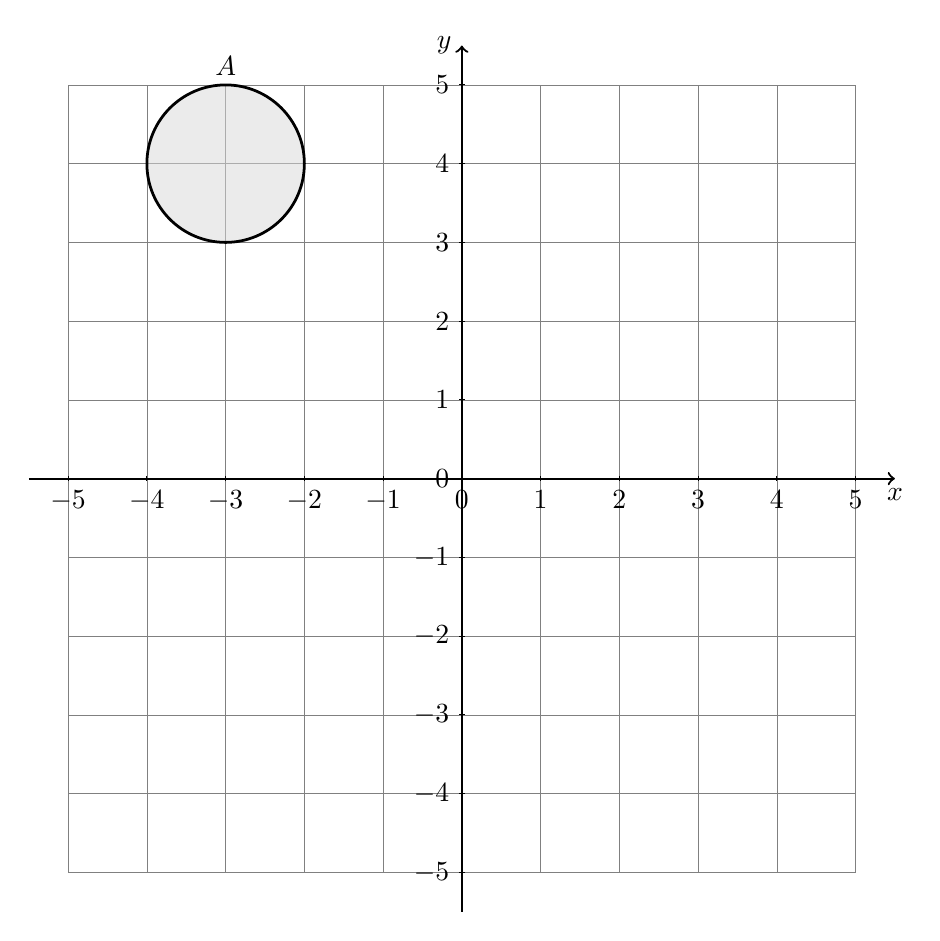
\begin{tikzpicture}[scale=1, transform shape]
    % Define colors
    \definecolor{borderColour}{HTML}{000000}
    \definecolor{fillColour}{HTML}{D8D8D8}
    
    % Define axis scale
    \def\axisLimit{5}

    % Draw grid
    \draw[step=1cm,gray,very thin] (-\axisLimit,-\axisLimit) grid (\axisLimit,\axisLimit);
    
    % Draw axes
    \draw[thick,->] (-\axisLimit-0.5,0) -- (\axisLimit+0.5,0) node[anchor=north] {$x$};
    \draw[thick,->] (0,-\axisLimit-0.5) -- (0,\axisLimit+0.5) node[anchor=east] {$y$};

    % Label x-axis, skip the 0 label
    \foreach \x in {-\axisLimit,...,\axisLimit}
        \draw (\x cm,1pt) -- (\x cm,-1pt) node[anchor=north] {$\x$};
    % Label y-axis, skip the 0 label
    \foreach \y in {-\axisLimit,...,\axisLimit}
        \draw (1pt,\y cm) -- (-1pt,\y cm) node[anchor=east] {$\y$};

    % Define the center of the first circle
    \coordinate (Center1) at (-3,4);
    % Draw the first circle using the center coordinate
    \filldraw[fill=fillColour, draw=borderColour, line width=1pt, fill opacity=0.5] (Center1) circle (1cm);
    % Label the first circle above the top of the circle
    \node[above] at ($(Center1)+(0,1)$) {$A$};

\end{tikzpicture}

% Q1 (solution)
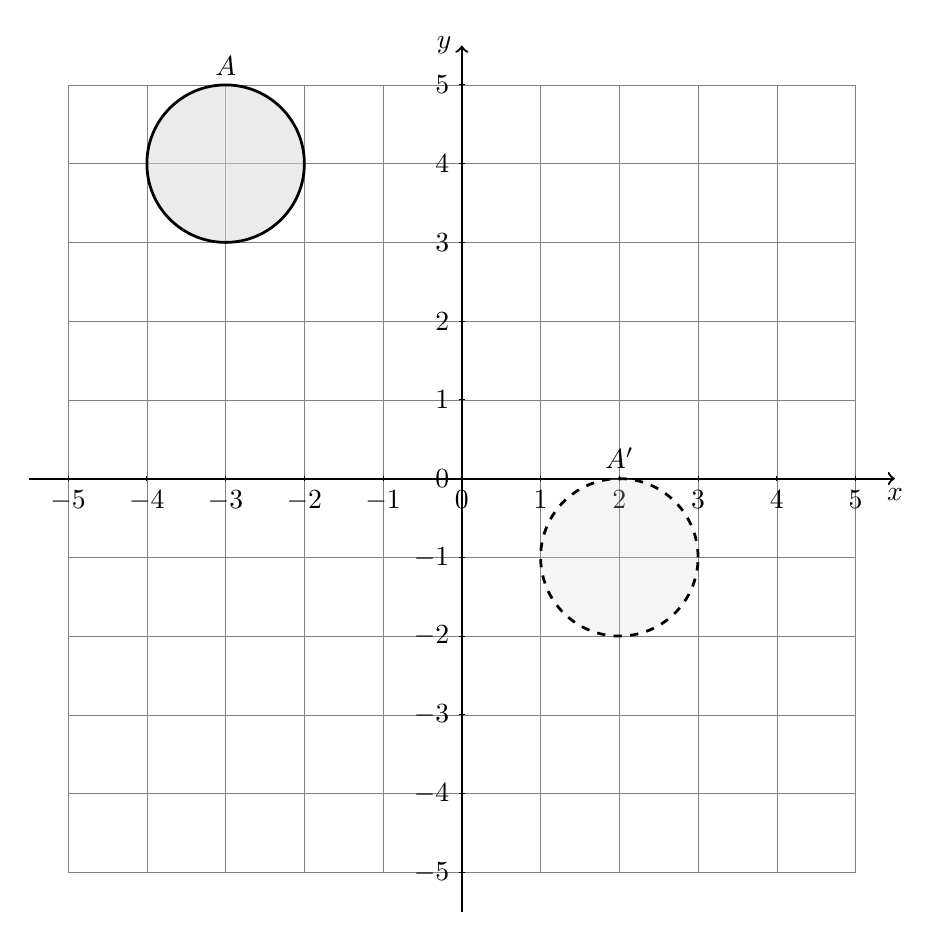
\begin{tikzpicture}[scale=1, transform shape]
    % Define colors
    \definecolor{borderColour}{HTML}{000000}
    \definecolor{fillColour}{HTML}{D8D8D8}
    
    % Define axis scale
    \def\axisLimit{5}

    % Draw grid
    \draw[step=1cm,gray,very thin] (-\axisLimit,-\axisLimit) grid (\axisLimit,\axisLimit);
    
    % Draw axes
    \draw[thick,->] (-\axisLimit-0.5,0) -- (\axisLimit+0.5,0) node[anchor=north] {$x$};
    \draw[thick,->] (0,-\axisLimit-0.5) -- (0,\axisLimit+0.5) node[anchor=east] {$y$};

    % Label x-axis, skip the 0 label
    \foreach \x in {-\axisLimit,...,\axisLimit}
        \draw (\x cm,1pt) -- (\x cm,-1pt) node[anchor=north] {$\x$};
    % Label y-axis, skip the 0 label
    \foreach \y in {-\axisLimit,...,\axisLimit}
        \draw (1pt,\y cm) -- (-1pt,\y cm) node[anchor=east] {$\y$};

    % Define the center of the first circle
    \coordinate (Center1) at (-3,4);
    % Draw the first circle using the center coordinate
    \filldraw[fill=fillColour, draw=borderColour, line width=1pt, fill opacity=0.5] (Center1) circle (1cm);
    % Label the first circle above the top of the circle
    \node[above] at ($(Center1)+(0,1)$) {$A$};

    % Define the center of the second circle
    \coordinate (Center2) at (2,-1);
    % Draw the second circle using the center coordinate
    \filldraw[fill=fillColour, draw=borderColour, line width=1pt, dashed, fill opacity=0.25] (Center2) circle (1cm);
    % Label the second circle above the top of the circle
    \node[above] at ($(Center2)+(0,1)$) {$A'$};

\end{tikzpicture}

% Q2 
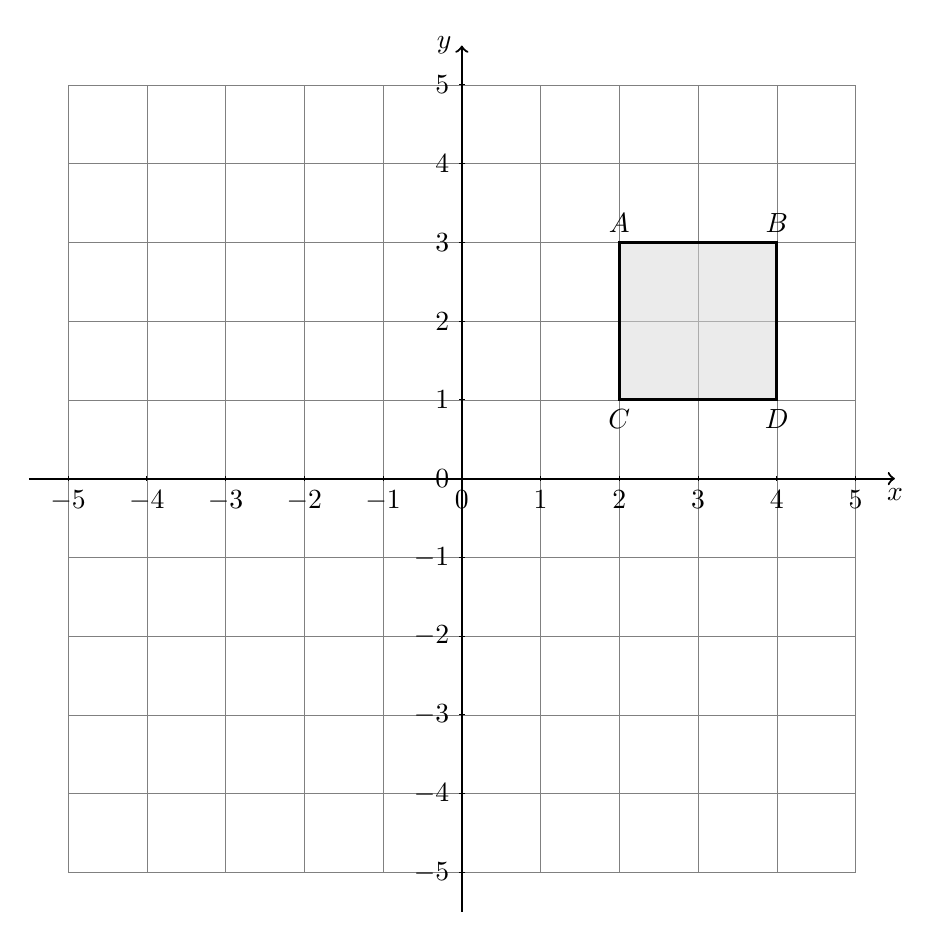
\begin{tikzpicture}[scale=1, transform shape]
    % Define colors
    \definecolor{borderColour}{HTML}{000000}
    \definecolor{fillColour}{HTML}{D8D8D8}
    
    % Define axis scale
    \def\axisLimit{5}

    % Draw grid
    \draw[step=1cm,gray,very thin] (-\axisLimit,-\axisLimit) grid (\axisLimit,\axisLimit);
    
    % Draw axes
    \draw[thick,->] (-\axisLimit-0.5,0) -- (\axisLimit+0.5,0) node[anchor=north] {$x$};
    \draw[thick,->] (0,-\axisLimit-0.5) -- (0,\axisLimit+0.5) node[anchor=east] {$y$};

    % Label x-axis, skip the 0 label
    \foreach \x in {-\axisLimit,...,\axisLimit}
        \draw (\x cm,1pt) -- (\x cm,-1pt) node[anchor=north] {$\x$};
    % Label y-axis, skip the 0 label
    \foreach \y in {-\axisLimit,...,\axisLimit}
        \draw (1pt,\y cm) -- (-1pt,\y cm) node[anchor=east] {$\y$};

    % Define coordinates for Square 1
    \coordinate (A1) at (2,3);
    \coordinate (B1) at ($(A1)+(2,0)$);
    \coordinate (C1) at ($(A1)+(0,-2)$);
    \coordinate (D1) at ($(B1)+(0,-2)$);

    % Draw Square 1
    \filldraw[fill=fillColour, draw=borderColour, line width=1pt, fill opacity=0.5] (A1) -- (B1) -- (D1) -- (C1) -- cycle;
    
    % Label corners of Square 1
    \node[above] at (A1) {$A$};
    \node[above] at (B1) {$B$};
    \node[below] at (C1) {$C$};
    \node[below] at (D1) {$D$};

\end{tikzpicture}

% Q2 (solution)
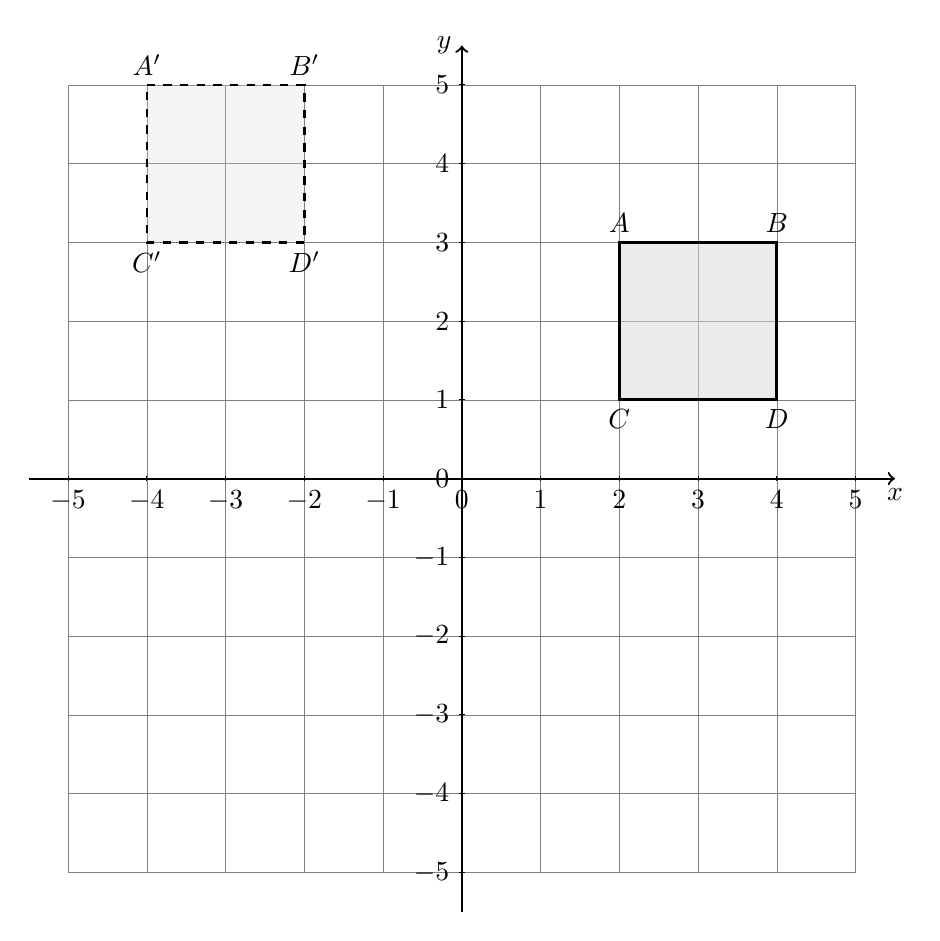
\begin{tikzpicture}[scale=1, transform shape]
    % Define colors
    \definecolor{borderColour}{HTML}{000000}
    \definecolor{fillColour}{HTML}{D8D8D8}
    
    % Define axis scale
    \def\axisLimit{5}

    % Draw grid
    \draw[step=1cm,gray,very thin] (-\axisLimit,-\axisLimit) grid (\axisLimit,\axisLimit);
    
    % Draw axes
    \draw[thick,->] (-\axisLimit-0.5,0) -- (\axisLimit+0.5,0) node[anchor=north] {$x$};
    \draw[thick,->] (0,-\axisLimit-0.5) -- (0,\axisLimit+0.5) node[anchor=east] {$y$};

    % Label x-axis, skip the 0 label
    \foreach \x in {-\axisLimit,...,\axisLimit}
        \draw (\x cm,1pt) -- (\x cm,-1pt) node[anchor=north] {$\x$};
    % Label y-axis, skip the 0 label
    \foreach \y in {-\axisLimit,...,\axisLimit}
        \draw (1pt,\y cm) -- (-1pt,\y cm) node[anchor=east] {$\y$};

    % Define coordinates for Square 1
    \coordinate (A1) at (2,3);
    \coordinate (B1) at ($(A1)+(2,0)$);
    \coordinate (C1) at ($(A1)+(0,-2)$);
    \coordinate (D1) at ($(B1)+(0,-2)$);

    % Draw Square 1
    \filldraw[fill=fillColour, draw=borderColour, line width=1pt, fill opacity=0.5] (A1) -- (B1) -- (D1) -- (C1) -- cycle;
    
    % Label corners of Square 1
    \node[above] at (A1) {$A$};
    \node[above] at (B1) {$B$};
    \node[below] at (C1) {$C$};
    \node[below] at (D1) {$D$};

    % Define coordinates for Square 2
    \coordinate (A2) at (-4,5);
    \coordinate (B2) at ($(A2)+(2,0)$);
    \coordinate (C2) at ($(A2)+(0,-2)$);
    \coordinate (D2) at ($(B2)+(0,-2)$);

    % Draw Square 2
    \filldraw[fill=fillColour, draw=borderColour, line width=1pt, fill opacity=0.25, dashed] (A2) -- (B2) -- (D2) -- (C2) -- cycle;
    
    % Label corners of Square 2
    \node[above] at (A2) {$A'$};
    \node[above] at (B2) {$B'$};
    \node[below] at (C2) {$C'$};
    \node[below] at (D2) {$D'$};

\end{tikzpicture}

% Q3
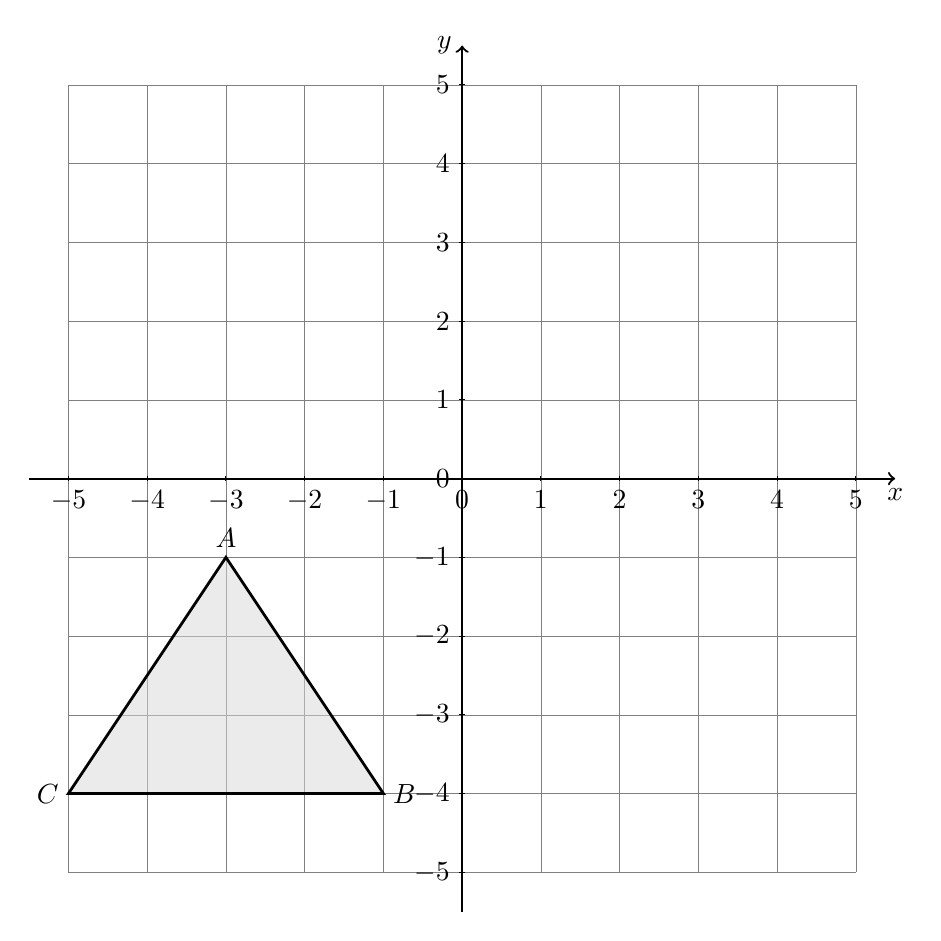
\begin{tikzpicture}[scale=1, transform shape]
    % Define colours
    \definecolor{borderColour}{HTML}{000000}
    \definecolor{fillColour}{HTML}{D8D8D8}
    
    % Define axis scale
    \def\axisLimit{5}

    % Draw grid
    \draw[step=1cm,gray,very thin] (-\axisLimit,-\axisLimit) grid (\axisLimit,\axisLimit);
    
    % Draw axes
    \draw[thick,->] (-\axisLimit-0.5,0) -- (\axisLimit+0.5,0) node[anchor=north] {$x$};
    \draw[thick,->] (0,-\axisLimit-0.5) -- (0,\axisLimit+0.5) node[anchor=east] {$y$};

    % Label x-axis, skip the 0 label
    \foreach \x in {-\axisLimit,...,\axisLimit}
        \draw (\x cm,1pt) -- (\x cm,-1pt) node[anchor=north] {$\x$};
    % Label y-axis, skip the 0 label
    \foreach \y in {-\axisLimit,...,\axisLimit}
        \draw (1pt,\y cm) -- (-1pt,\y cm) node[anchor=east] {$\y$};

    % Define coordinates for the vertices of the first triangle
    \coordinate (A) at (-3,-1);
    \coordinate (B) at (-1,-4);
    \coordinate (C) at (-5,-4);

    % Draw the first triangle using the defined coordinates
    \filldraw[fill=fillColour, draw=borderColour, line width=1pt, fill opacity=0.5] (A) -- (B) -- (C) -- cycle;
    
    % Label the vertices of the first triangle
    \node[above] at (A) {$A$};
    \node[right] at (B) {$B$};
    \node[left] at (C) {$C$};

\end{tikzpicture}

% Q3 (solution)
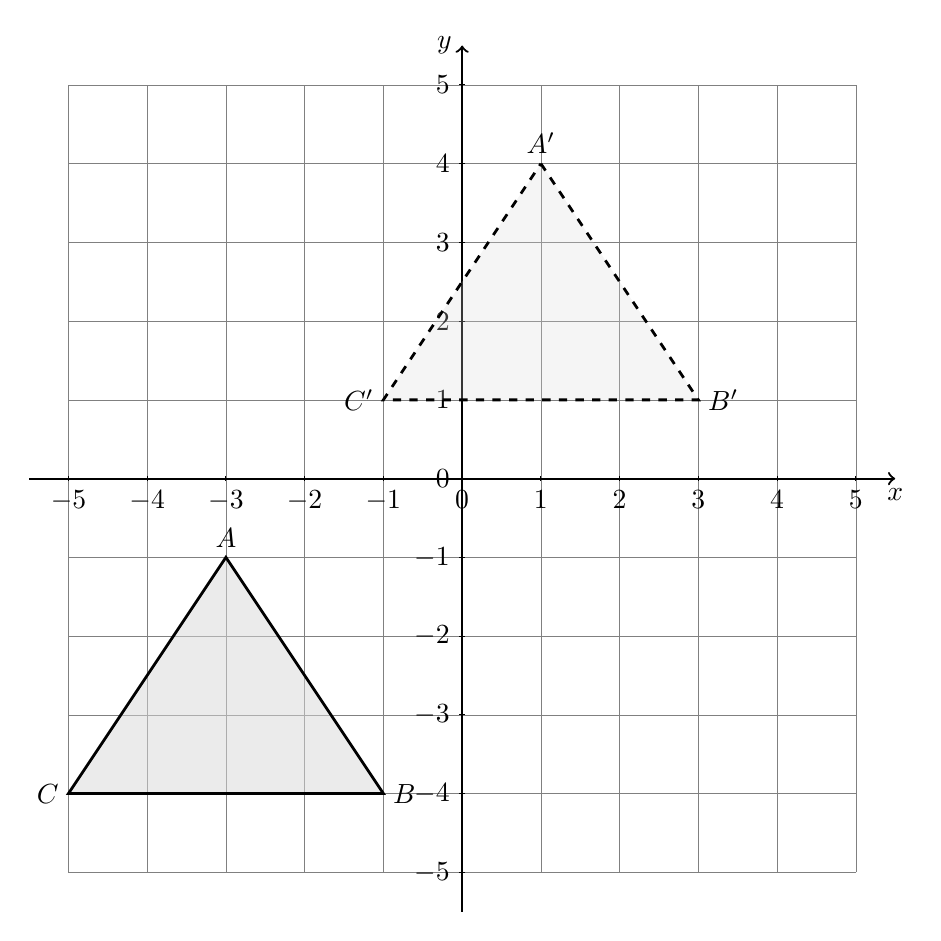
\begin{tikzpicture}[scale=1, transform shape]
    % Define colours
    \definecolor{borderColour}{HTML}{000000}
    \definecolor{fillColour}{HTML}{D8D8D8}
    
    % Define axis scale
    \def\axisLimit{5}

    % Draw grid
    \draw[step=1cm,gray,very thin] (-\axisLimit,-\axisLimit) grid (\axisLimit,\axisLimit);
    
    % Draw axes
    \draw[thick,->] (-\axisLimit-0.5,0) -- (\axisLimit+0.5,0) node[anchor=north] {$x$};
    \draw[thick,->] (0,-\axisLimit-0.5) -- (0,\axisLimit+0.5) node[anchor=east] {$y$};

    % Label x-axis, skip the 0 label
    \foreach \x in {-\axisLimit,...,\axisLimit}
        \draw (\x cm,1pt) -- (\x cm,-1pt) node[anchor=north] {$\x$};
    % Label y-axis, skip the 0 label
    \foreach \y in {-\axisLimit,...,\axisLimit}
        \draw (1pt,\y cm) -- (-1pt,\y cm) node[anchor=east] {$\y$};

    % Define coordinates for the vertices of the second triangle
    \coordinate (A) at (-3,-1);
    \coordinate (B) at (-1,-4);
    \coordinate (C) at (-5,-4);

    % Draw the second triangle using the defined coordinates
    \filldraw[fill=fillColour, draw=borderColour, line width=1pt, fill opacity=0.5] (A) -- (B) -- (C) -- cycle;
    
    % Label the vertices of the second triangle
    \node[above] at (A) {$A$};
    \node[right] at (B) {$B$};
    \node[left] at (C) {$C$};

    % Define coordinates for the vertices of the first triangle
    \coordinate (A') at (1,4);
    \coordinate (B') at (3,1);
    \coordinate (C') at (-1,1);

    % Draw the first triangle using the defined coordinates
    \filldraw[dashed, fill=fillColour, draw=borderColour, line width=1pt, fill opacity=0.25] (A') -- (B') -- (C') -- cycle;
    
    % Label the vertices of the first triangle
    \node[above] at (A') {$A'$};
    \node[right] at (B') {$B'$};
    \node[left] at (C') {$C'$};

\end{tikzpicture}

% Q4
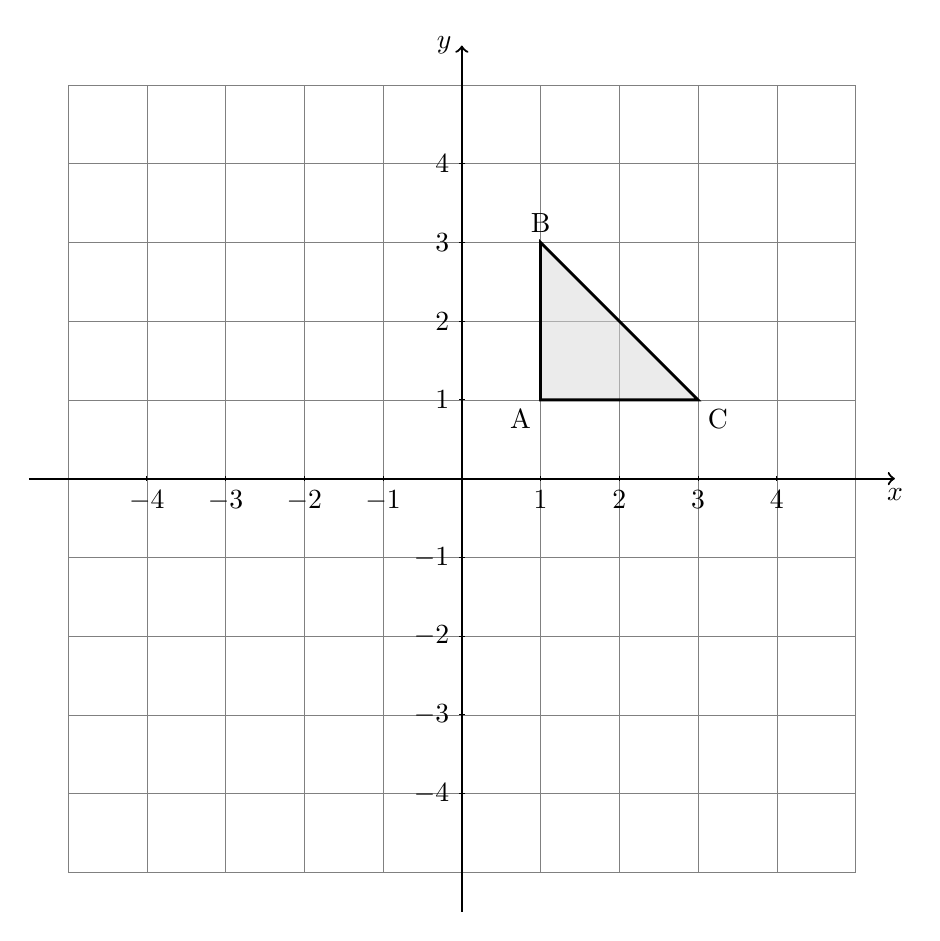
\begin{tikzpicture}[scale=1]
    % Define colours
    \definecolor{borderColour}{HTML}{000000}
    \definecolor{fillColour}{HTML}{D8D8D8}
    
    % Define axis scale
    \def\axisLimit{5}

  % Draw the grid
  \draw[step=1cm,gray,very thin] (-\axisLimit,-\axisLimit) grid (\axisLimit,\axisLimit);
  \draw[thick,->] (-\axisLimit-0.5,0) -- (\axisLimit+0.5,0) node[anchor=north] {$x$};
  \draw[thick,->] (0,-\axisLimit-0.5) -- (0,\axisLimit+0.5) node[anchor=east] {$y$};

  % Label x-axis and y-axis from -4 to 4, skipping 0
  \foreach \x in {-4,-3,...,-1,1,2,...,4}
    \draw (\x cm,1pt) -- (\x cm,-1pt) node[anchor=north] {$\x$};
  \foreach \y in {-4,-3,...,-1,1,2,...,4}
    \draw (1pt,\y cm) -- (-1pt,\y cm) node[anchor=east] {$\y$};

  % Define the vertices of the original triangle
  \coordinate (A) at (1,1);
  \coordinate (B) at (1,3);
  \coordinate (C) at (3,1);

  % Draw the original triangle
  \filldraw[fill=fillColour, draw=borderColour, line width=1pt, fill opacity=0.5] (A) -- (B) -- (C) -- cycle;

  % Label the original and translated triangles
  \node[below left] at (A) {A};
  \node[above] at (B) {B};
  \node[below right] at (C) {C};
  
\end{tikzpicture}

% Q4 (solution)
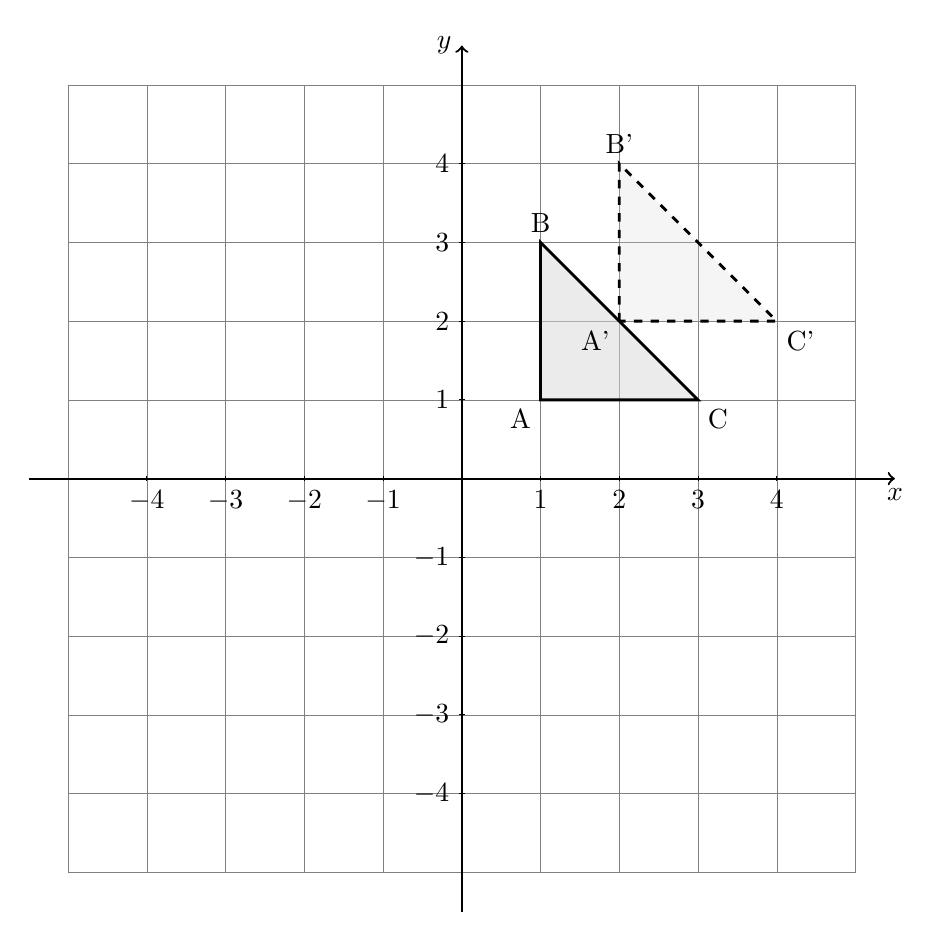
\begin{tikzpicture}[scale=1]
    % Define colours
    \definecolor{borderColour}{HTML}{000000}
    \definecolor{fillColour}{HTML}{D8D8D8}
    
    % Define axis scale
    \def\axisLimit{5}

  % Draw the grid
  \draw[step=1cm,gray,very thin] (-\axisLimit,-\axisLimit) grid (\axisLimit,\axisLimit);
  \draw[thick,->] (-\axisLimit-0.5,0) -- (\axisLimit+0.5,0) node[anchor=north] {$x$};
  \draw[thick,->] (0,-\axisLimit-0.5) -- (0,\axisLimit+0.5) node[anchor=east] {$y$};

  % Label x-axis and y-axis from -4 to 4, skipping 0
  \foreach \x in {-4,-3,...,-1,1,2,...,4}
    \draw (\x cm,1pt) -- (\x cm,-1pt) node[anchor=north] {$\x$};
  \foreach \y in {-4,-3,...,-1,1,2,...,4}
    \draw (1pt,\y cm) -- (-1pt,\y cm) node[anchor=east] {$\y$};

  % Define the vertices of the original triangle
  \coordinate (A) at (1,1);
  \coordinate (B) at (1,3);
  \coordinate (C) at (3,1);

  % Draw the original triangle
  \filldraw[fill=fillColour, draw=borderColour, line width=1pt, fill opacity=0.5] (A) -- (B) -- (C) -- cycle;

  % Define the vertices of the translated triangle
  \coordinate (A') at ($(A)+(1,1)$);
  \coordinate (B') at ($(B)+(1,1)$);
  \coordinate (C') at ($(C)+(1,1)$);

  % Draw the translated triangle
  \filldraw[fill=fillColour, draw=borderColour, line width=1pt, fill opacity=0.25, dashed] (A') -- (B') -- (C') -- cycle;

  % Label the original and translated triangles
  \node[below left] at (A) {A};
  \node[above] at (B) {B};
  \node[below right] at (C) {C};
  \node[below left] at (A') {A'};
  \node[above] at (B') {B'};
  \node[below right] at (C') {C'};
  
\end{tikzpicture}

% Q5 (solution)
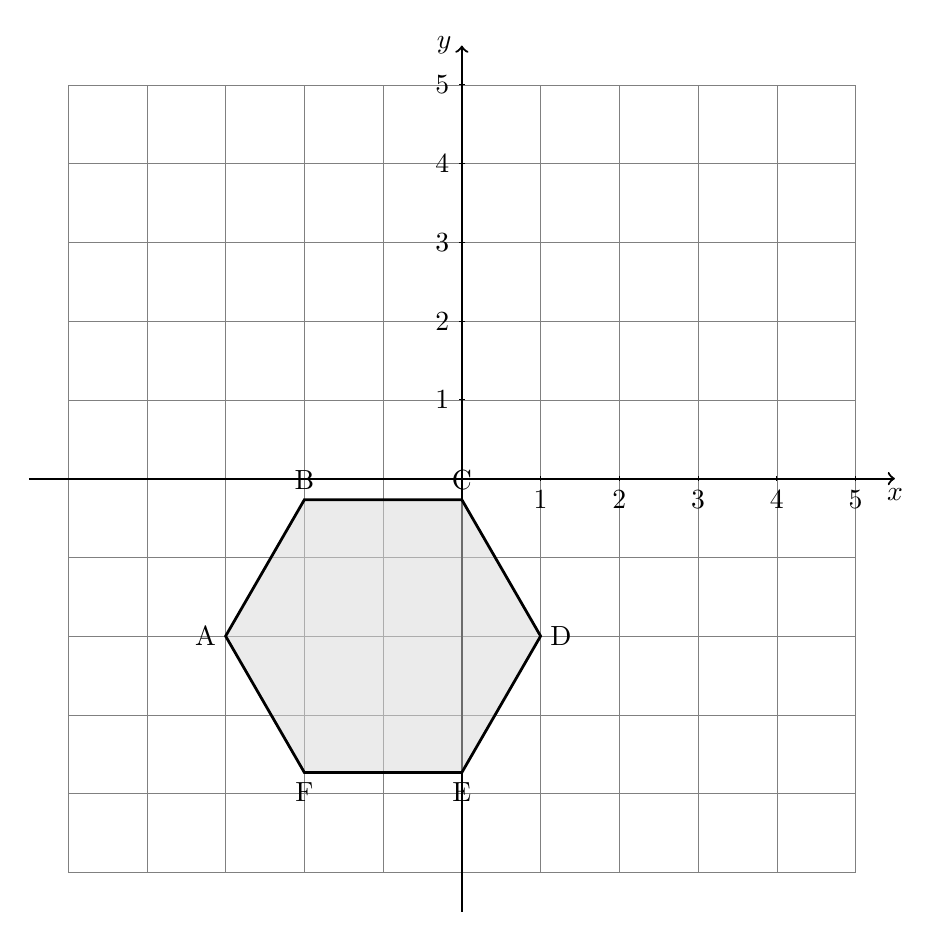
\begin{tikzpicture}[scale=1]
    % Define colours
    \definecolor{borderColour}{HTML}{000000}
    \definecolor{fillColour}{HTML}{D8D8D8}
    
    % Macros for the initial position of A and the transformation vector
    \def\initialAx{-3} % X part of the initial position
    \def\initialAy{-2} % Y part of the initial position
    \def\hexagonSide{2} % Side length of the hexagon
    \def\transformationX{4} % X part of the transformation vector
    \def\transformationY{5}  % Y part of the transformation vector
    
    % Define axis scale
    \def\axisLimit{5}

  % Draw the grid
  \draw[step=1cm,gray,very thin] (-\axisLimit,-\axisLimit) grid (\axisLimit,\axisLimit);
  \draw[thick,->] (-\axisLimit-0.5,0) -- (\axisLimit+0.5,0) node[anchor=north] {$x$};
  \draw[thick,->] (0,-\axisLimit-0.5) -- (0,\axisLimit+0.5) node[anchor=east] {$y$};

  % Label x-axis, skip the 0 label
    \foreach \x in {1,2,...,5}
        \draw (\x cm,1pt) -- (\x cm,-1pt) node[anchor=north] {$\x$};
    % Label y-axis, skip the 0 label
    \foreach \y in {1,2,...,5}
        \draw (1pt,\y cm) -- (-1pt,\y cm) node[anchor=east] {$\y$};

  % Define the initial vertex of the original hexagon using the macro
  \coordinate (A) at (\initialAx,\initialAy);

  % Define the remaining vertices of the original hexagon dynamically
  \coordinate (B) at ($(A) + (60:\hexagonSide)$); % 60 degrees from A
  \coordinate (C) at ($(B) + (0:\hexagonSide)$);  % 0 degrees from B
  \coordinate (D) at ($(C) + (-60:\hexagonSide)$); % -60 degrees from C
  \coordinate (E) at ($(D) + (-120:\hexagonSide)$); % -120 degrees from D
  \coordinate (F) at ($(E) + (180:\hexagonSide)$); % 180 degrees from E

  % Draw the original hexagon
  \filldraw[fill=fillColour, draw=borderColour, line width=1pt, fill opacity=0.5] (A) -- (B) -- (C) -- (D) -- (E) -- (F) -- cycle;

  % Label the original hexagon vertices
  \path (A) node[left] {A};
  \path (B) node[above] {B};
  \path (C) node[above] {C};
  \path (D) node[right] {D};
  \path (E) node[below] {E};
  \path (F) node[below] {F};

\end{tikzpicture}

% Q5
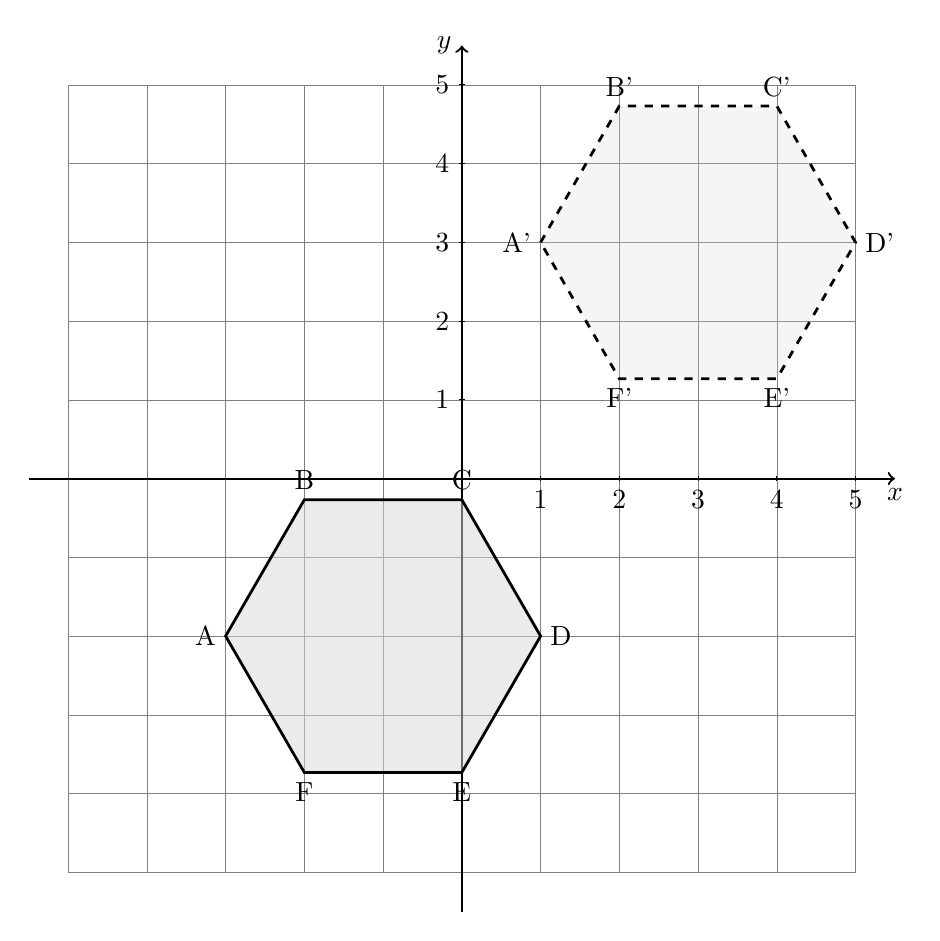
\begin{tikzpicture}[scale=1]
    % Define colours
    \definecolor{borderColour}{HTML}{000000}
    \definecolor{fillColour}{HTML}{D8D8D8}
    
    % Macros for the initial position of A and the transformation vector
    \def\initialAx{-3} % X part of the initial position
    \def\initialAy{-2} % Y part of the initial position
    \def\hexagonSide{2} % Side length of the hexagon
    \def\transformationX{4} % X part of the transformation vector
    \def\transformationY{5}  % Y part of the transformation vector
    
    % Define axis scale
    \def\axisLimit{5}

  % Draw the grid
  \draw[step=1cm,gray,very thin] (-\axisLimit,-\axisLimit) grid (\axisLimit,\axisLimit);
  \draw[thick,->] (-\axisLimit-0.5,0) -- (\axisLimit+0.5,0) node[anchor=north] {$x$};
  \draw[thick,->] (0,-\axisLimit-0.5) -- (0,\axisLimit+0.5) node[anchor=east] {$y$};

  % Label x-axis, skip the 0 label
    \foreach \x in {1,2,...,5}
        \draw (\x cm,1pt) -- (\x cm,-1pt) node[anchor=north] {$\x$};
    % Label y-axis, skip the 0 label
    \foreach \y in {1,2,...,5}
        \draw (1pt,\y cm) -- (-1pt,\y cm) node[anchor=east] {$\y$};

  % Define the initial vertex of the original hexagon using the macro
  \coordinate (A) at (\initialAx,\initialAy);

  % Define the remaining vertices of the original hexagon dynamically
  \coordinate (B) at ($(A) + (60:\hexagonSide)$); % 60 degrees from A
  \coordinate (C) at ($(B) + (0:\hexagonSide)$);  % 0 degrees from B
  \coordinate (D) at ($(C) + (-60:\hexagonSide)$); % -60 degrees from C
  \coordinate (E) at ($(D) + (-120:\hexagonSide)$); % -120 degrees from D
  \coordinate (F) at ($(E) + (180:\hexagonSide)$); % 180 degrees from E

  % Draw the original hexagon
  \filldraw[fill=fillColour, draw=borderColour, line width=1pt, fill opacity=0.5] (A) -- (B) -- (C) -- (D) -- (E) -- (F) -- cycle;

  % Apply the transformation to the original vertices
  \coordinate (A') at ($(A) + (\transformationX,\transformationY)$);
  \coordinate (B') at ($(B) + (\transformationX,\transformationY)$);
  \coordinate (C') at ($(C) + (\transformationX,\transformationY)$);
  \coordinate (D') at ($(D) + (\transformationX,\transformationY)$);
  \coordinate (E') at ($(E) + (\transformationX,\transformationY)$);
  \coordinate (F') at ($(F) + (\transformationX,\transformationY)$);

  % Draw the translated hexagon
  \filldraw[fill=fillColour, draw=borderColour, line width=1pt, fill opacity=0.25, dashed] (A') -- (B') -- (C') -- (D') -- (E') -- (F') -- cycle;

  % Label the original and translated hexagon vertices
  % Label the original hexagon vertices
  \path (A) node[left] {A};
  \path (B) node[above] {B};
  \path (C) node[above] {C};
  \path (D) node[right] {D};
  \path (E) node[below] {E};
  \path (F) node[below] {F};

  % Label the translated hexagon vertices
  \path (A') node[left] {A'};
  \path (B') node[above] {B'};
  \path (C') node[above] {C'};
  \path (D') node[right] {D'};
  \path (E') node[below] {E'};
  \path (F') node[below] {F'};

\end{tikzpicture}

% Q6
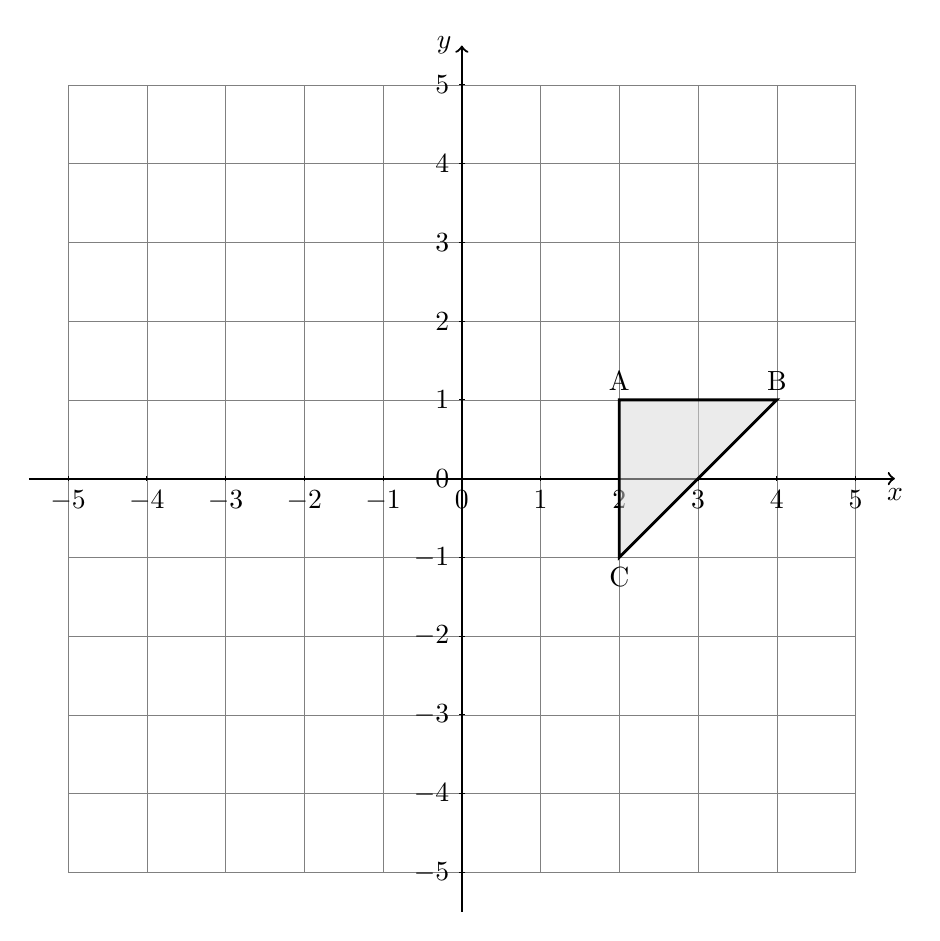
\begin{tikzpicture}[scale=1, transform shape]
    % Define colours
    \definecolor{borderColour}{HTML}{000000}
    \definecolor{fillColour}{HTML}{D8D8D8}

    % Define axis scale
    \def\axisLimit{5}

    % Draw grid
    \draw[step=1cm,gray,very thin] (-\axisLimit,-\axisLimit) grid (\axisLimit,\axisLimit);
    
    % Draw axes
    \draw[thick,->] (-\axisLimit-0.5,0) -- (\axisLimit+0.5,0) node[anchor=north] {$x$};
    \draw[thick,->] (0,-\axisLimit-0.5) -- (0,\axisLimit+0.5) node[anchor=east] {$y$};

    % Label x-axis and y-axis from -4 to 4, skipping label at 0
    \foreach \x in {-\axisLimit,...,\axisLimit}
        \draw (\x cm,1pt) -- (\x cm,-1pt) node[anchor=north] {$\x$};
    \foreach \y in {-\axisLimit,...,\axisLimit}
        \draw (1pt,\y cm) -- (-1pt,\y cm) node[anchor=east] {$\y$};

    % Define coordinates for the vertices of the original triangle
    \coordinate (A) at (2,1);
    \coordinate (B) at (4,1);
    \coordinate (C) at (2,-1);

    % Draw the original triangle
    \filldraw[fill=fillColour, draw=borderColour, line width=1pt, fill opacity=0.5] (A) -- (B) -- (C) -- cycle;


    % Label the vertices of the original triangle
    \node[above] at (A) {A};
    \node[above] at (B) {B};
    \node[below] at (C) {C};

\end{tikzpicture}

% Q6 (solution)
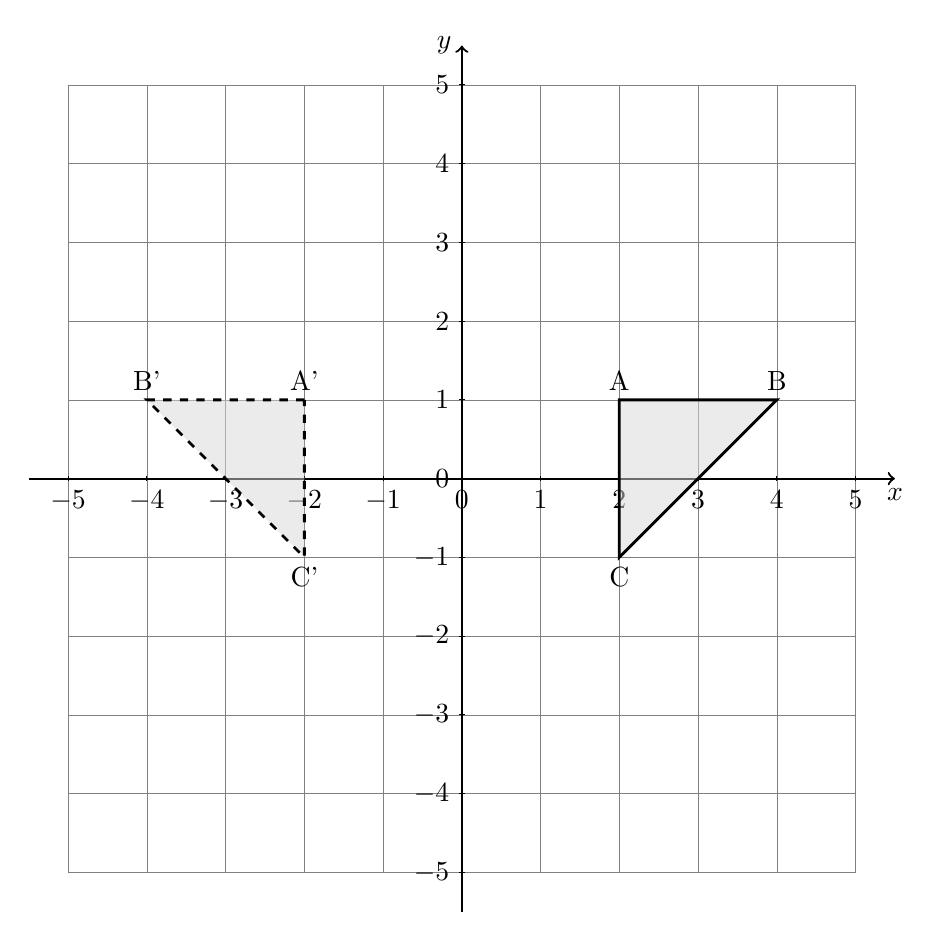
\begin{tikzpicture}[scale=1, transform shape]
    % Define colours
    \definecolor{borderColour}{HTML}{000000}
    \definecolor{fillColour}{HTML}{D8D8D8}

    % Define axis scale
    \def\axisLimit{5}

    % Draw grid
    \draw[step=1cm,gray,very thin] (-\axisLimit,-\axisLimit) grid (\axisLimit,\axisLimit);
    
    % Draw axes
    \draw[thick,->] (-\axisLimit-0.5,0) -- (\axisLimit+0.5,0) node[anchor=north] {$x$};
    \draw[thick,->] (0,-\axisLimit-0.5) -- (0,\axisLimit+0.5) node[anchor=east] {$y$};

    % Label x-axis and y-axis from -4 to 4, skipping label at 0
    \foreach \x in {-\axisLimit,...,\axisLimit}
        \draw (\x cm,1pt) -- (\x cm,-1pt) node[anchor=north] {$\x$};
    \foreach \y in {-\axisLimit,...,\axisLimit}
        \draw (1pt,\y cm) -- (-1pt,\y cm) node[anchor=east] {$\y$};

    % Draw the reflection line (y-axis in this case)
    \draw[thick,dotted] (0,-5) -- (0,5);

    % Define coordinates for the vertices of the original triangle
    \coordinate (A) at (2,1);
    \coordinate (B) at (4,1);
    \coordinate (C) at (2,-1);

    % Draw the original triangle
    \filldraw[fill=fillColour, draw=borderColour, line width=1pt, fill opacity=0.5] (A) -- (B) -- (C) -- cycle;


    % Label the vertices of the original triangle
    \node[above] at (A) {A};
    \node[above] at (B) {B};
    \node[below] at (C) {C};

    % Reflect the triangle over the y-axis by changing the sign of x-coordinates
    \coordinate (A') at (-2,1);
    \coordinate (B') at (-4,1);
    \coordinate (C') at (-2,-1);

    % Draw the reflected triangle
    \filldraw[dashed, fill=fillColour, draw=borderColour, line width=1pt, fill opacity=0.5] (A') -- (B') -- (C') -- cycle;

    % Label the vertices of the reflected triangle
    \node[above] at (A') {A'};
    \node[above] at (B') {B'};
    \node[below] at (C') {C'};

\end{tikzpicture}

% Q7
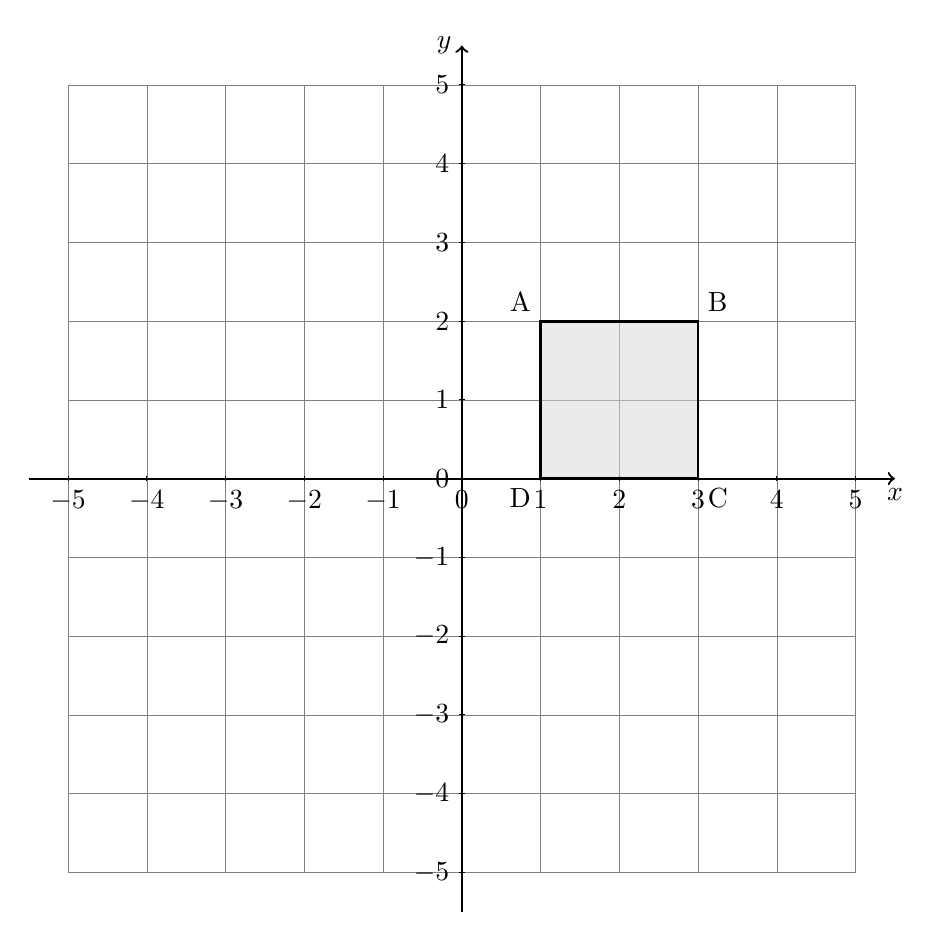
\begin{tikzpicture}[scale=1, transform shape]
    % Define colours
    \definecolor{borderColour}{HTML}{000000}
    \definecolor{fillColour}{HTML}{D8D8D8}
    
    % Define axis scale
    \def\axisLimit{5}

    % Draw grid
    \draw[step=1cm,gray,very thin] (-\axisLimit,-\axisLimit) grid (\axisLimit,\axisLimit);
    
    % Draw axes
    \draw[thick,->] (-\axisLimit-0.5,0) -- (\axisLimit+0.5,0) node[anchor=north] {$x$};
    \draw[thick,->] (0,-\axisLimit-0.5) -- (0,\axisLimit+0.5) node[anchor=east] {$y$};

    % Label x-axis and y-axis
    \foreach \x in {-\axisLimit,...,\axisLimit}
        \draw (\x cm,1pt) -- (\x cm,-1pt) node[anchor=north] {$\x$};
    \foreach \y in {-\axisLimit,...,\axisLimit}
        \draw (1pt,\y cm) -- (-1pt,\y cm) node[anchor=east] {$\y$};

    % Define coordinates for the vertices of the original rectangle
    \coordinate (A) at (1,2);
    \coordinate (B) at (3,2);
    \coordinate (C) at (3,0);
    \coordinate (D) at (1,0);

    % Draw the original rectangle
    \filldraw[fill=fillColour, draw=borderColour, line width=1pt, fill opacity=0.5] (A) -- (B) -- (C) -- (D) -- cycle;

    % Label the vertices of the original rectangle
    \node[above left] at (A) {A};
    \node[above right] at (B) {B};
    \node[below right] at (C) {C};
    \node[below left] at (D) {D};
    
\end{tikzpicture}

% Q7 (solution)
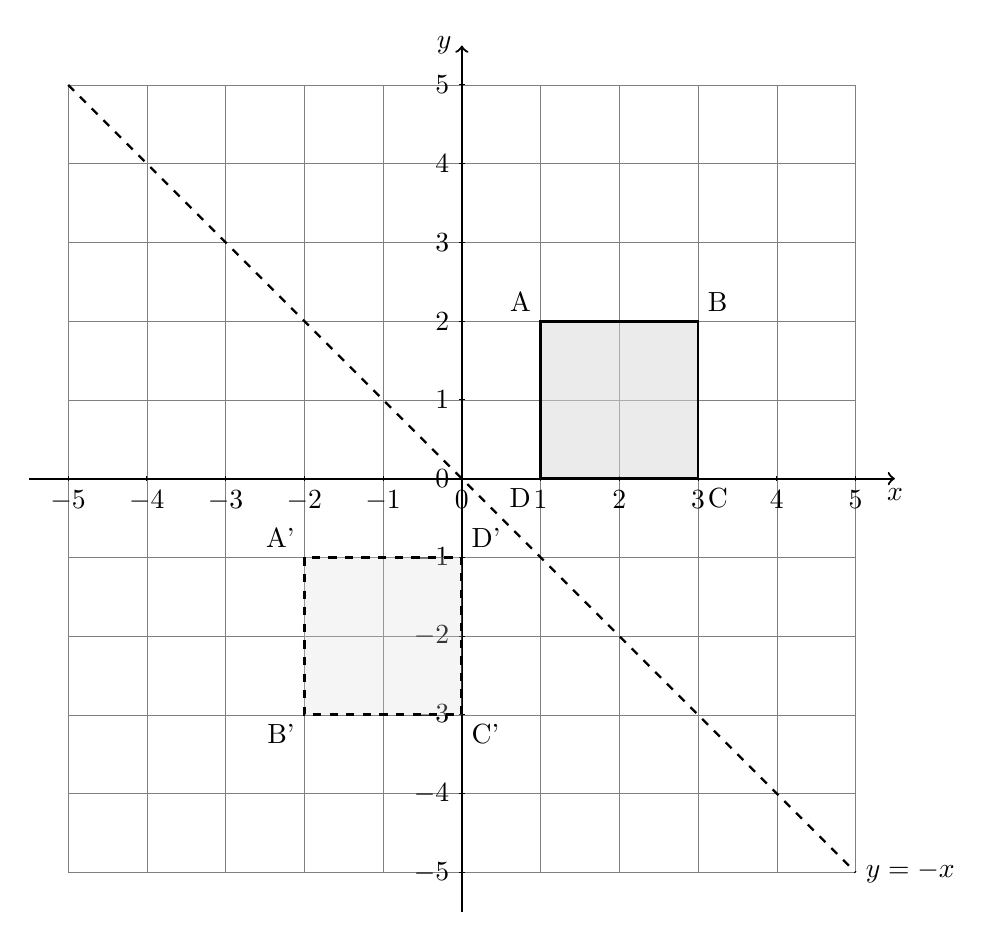
\begin{tikzpicture}[scale=1, transform shape]
    % Define colours
    \definecolor{borderColour}{HTML}{000000}
    \definecolor{fillColour}{HTML}{D8D8D8}
    
    % Define axis scale
    \def\axisLimit{5}

    % Draw grid
    \draw[step=1cm,gray,very thin] (-\axisLimit,-\axisLimit) grid (\axisLimit,\axisLimit);
    
    % Draw axes
    \draw[thick,->] (-\axisLimit-0.5,0) -- (\axisLimit+0.5,0) node[anchor=north] {$x$};
    \draw[thick,->] (0,-\axisLimit-0.5) -- (0,\axisLimit+0.5) node[anchor=east] {$y$};

    % Label x-axis and y-axis
    \foreach \x in {-\axisLimit,...,\axisLimit}
        \draw (\x cm,1pt) -- (\x cm,-1pt) node[anchor=north] {$\x$};
    \foreach \y in {-\axisLimit,...,\axisLimit}
        \draw (1pt,\y cm) -- (-1pt,\y cm) node[anchor=east] {$\y$};

    % Draw the reflection line y = -x
    \draw[thick,dashed] (-5,5) -- (5,-5) node[anchor=west] {$y=-x$};

    % Define coordinates for the vertices of the original rectangle
    \coordinate (A) at (1,2);
    \coordinate (B) at (3,2);
    \coordinate (C) at (3,0);
    \coordinate (D) at (1,0);

    % Draw the original rectangle
    \filldraw[fill=fillColour, draw=borderColour, line width=1pt, fill opacity=0.5] (A) -- (B) -- (C) -- (D) -- cycle;

    % Label the vertices of the original rectangle
    \node[above left] at (A) {A};
    \node[above right] at (B) {B};
    \node[below right] at (C) {C};
    \node[below left] at (D) {D};

    % Reflect the rectangle over the line y = -x
    \coordinate (A') at (-2,-1);
    \coordinate (B') at (-2,-3);
    \coordinate (C') at (0,-3);
    \coordinate (D') at (0,-1);

    % Draw the reflected rectangle
    \filldraw[fill=fillColour, draw=borderColour, line width=1pt, fill opacity=0.25, dashed] (A') -- (B') -- (C') -- (D') -- cycle;

    % Label the vertices of the reflected rectangle
    \node[above left] at (A') {A'};
    \node[below left] at (B') {B'};
    \node[below right] at (C') {C'};
    \node[above right] at (D') {D'};
    
\end{tikzpicture}

% Q8
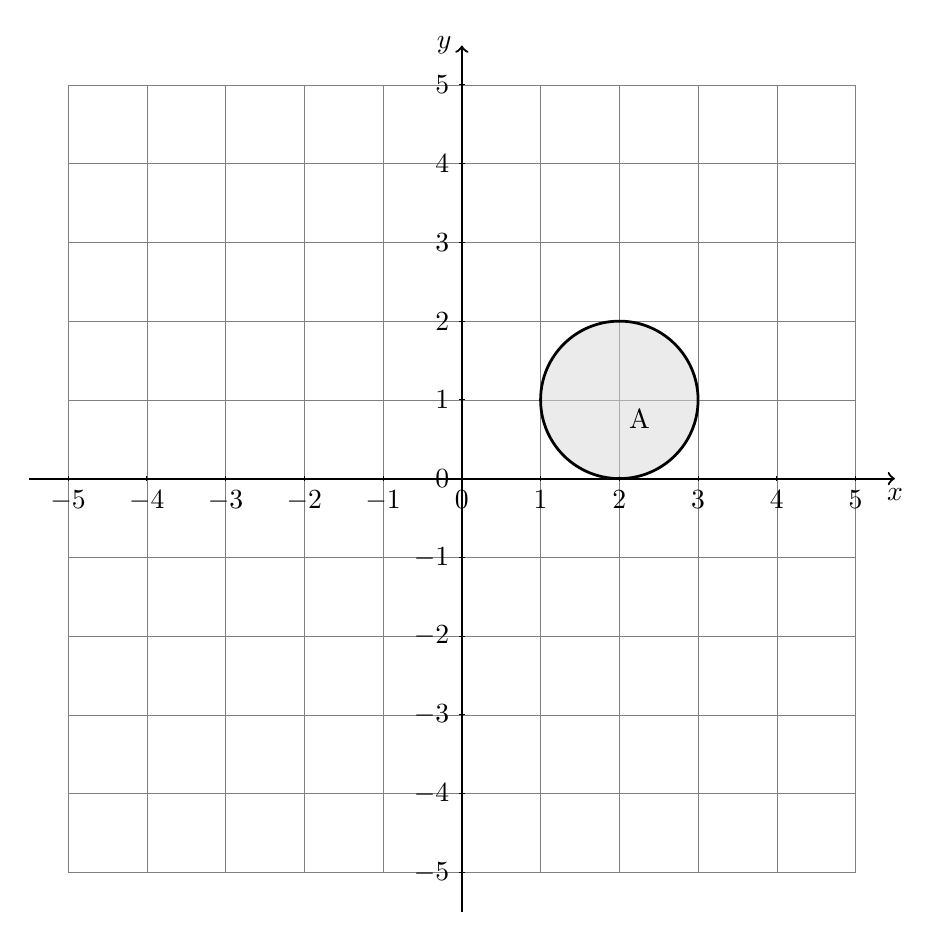
\begin{tikzpicture}[scale=1, transform shape]
    % Define colours
    \definecolor{borderColour}{HTML}{000000}
    \definecolor{fillColour}{HTML}{D8D8D8}
    
    % Define axis scale
    \def\axisLimit{5}

    % Draw grid
    \draw[step=1cm,gray,very thin] (-\axisLimit,-\axisLimit) grid (\axisLimit,\axisLimit);
    
    % Draw axes
    \draw[thick,->] (-\axisLimit-0.5,0) -- (\axisLimit+0.5,0) node[anchor=north] {$x$};
    \draw[thick,->] (0,-\axisLimit-0.5) -- (0,\axisLimit+0.5) node[anchor=east] {$y$};

    % Label x-axis and y-axis
    \foreach \x in {-\axisLimit,...,\axisLimit}
        \draw (\x cm,1pt) -- (\x cm,-1pt) node[anchor=north] {$\x$};
    \foreach \y in {-\axisLimit,...,\axisLimit}
        \draw (1pt,\y cm) -- (-1pt,\y cm) node[anchor=east] {$\y$};

    % Define coordinates for the center of the original circle
    \coordinate (A) at (2,1);

    % Draw the original circle
    \filldraw[fill=fillColour, draw=borderColour, line width=1pt, fill opacity=0.5] (A) circle (1cm);

    % Label the center of the original circle
    \node[below right] at (A) {A};
    
\end{tikzpicture}

% Q8 (solution)
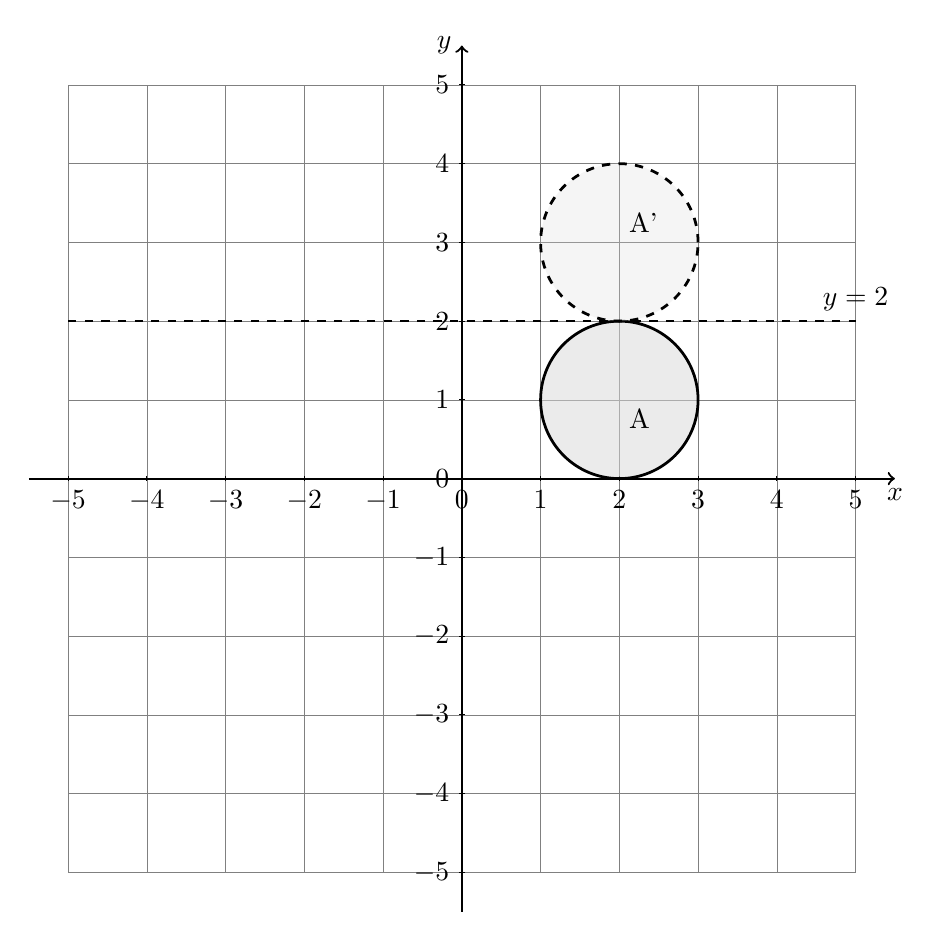
\begin{tikzpicture}[scale=1, transform shape]
    % Define colours
    \definecolor{borderColour}{HTML}{000000}
    \definecolor{fillColour}{HTML}{D8D8D8}
    
    % Define axis scale
    \def\axisLimit{5}

    % Draw grid
    \draw[step=1cm,gray,very thin] (-\axisLimit,-\axisLimit) grid (\axisLimit,\axisLimit);
    
    % Draw axes
    \draw[thick,->] (-\axisLimit-0.5,0) -- (\axisLimit+0.5,0) node[anchor=north] {$x$};
    \draw[thick,->] (0,-\axisLimit-0.5) -- (0,\axisLimit+0.5) node[anchor=east] {$y$};

    % Label x-axis and y-axis
    \foreach \x in {-\axisLimit,...,\axisLimit}
        \draw (\x cm,1pt) -- (\x cm,-1pt) node[anchor=north] {$\x$};
    \foreach \y in {-\axisLimit,...,\axisLimit}
        \draw (1pt,\y cm) -- (-1pt,\y cm) node[anchor=east] {$\y$};

    % Draw the reflection line y = 2
    \draw[thick,dashed] (-5,2) -- (5,2) node[anchor=south] {$y=2$};

    % Define coordinates for the center of the original circle
    \coordinate (A) at (2,1);

    % Draw the original circle
    \filldraw[fill=fillColour, draw=borderColour, line width=1pt, fill opacity=0.5] (A) circle (1cm);

    % Label the center of the original circle
    \node[below right] at (A) {A};

    % Reflect the circle over the line y = 2
    % The reflected center is (2, 3) as the original center (2, 1) is 1 unit below y = 2
    \coordinate (A') at (2,3);

    % Draw the reflected circle
    \filldraw[dashed, fill=fillColour, draw=borderColour, line width=1pt, fill opacity=0.25] (A') circle (1cm);

    % Label the center of the reflected circle
    \node[above right] at (A') {A'};
    
\end{tikzpicture}

% Q9 
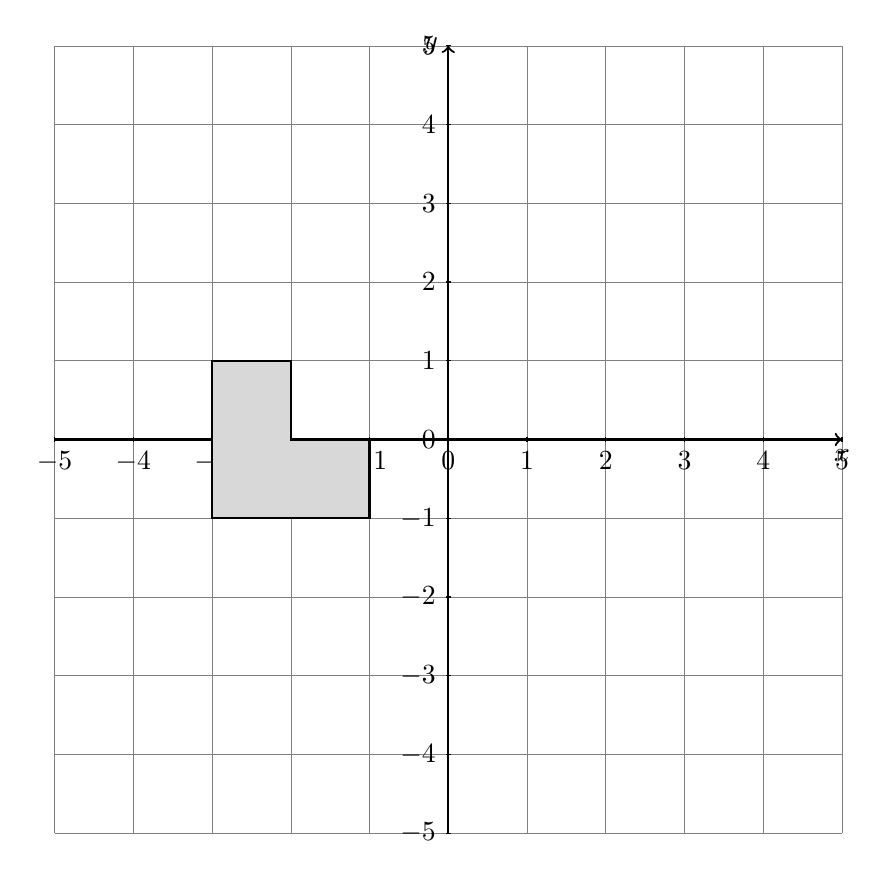
\begin{tikzpicture}[scale=1, transform shape]
    % Define colours
    \definecolor{borderColour}{HTML}{000000}
    \definecolor{fillColour}{HTML}{D8D8D8}
    
    % Define axis scale
    \def\axisLimit{5}

    % Draw grid
    \draw[step=1cm,gray,very thin] (-\axisLimit,-\axisLimit) grid (\axisLimit,\axisLimit);
    
    % Draw axes
    \draw[thick,->] (-5,0) -- (5,0) node[anchor=north] {$x$};
    \draw[thick,->] (0,-5) -- (0,5) node[anchor=east] {$y$};

    % Label x-axis and y-axis
    \foreach \x in {-\axisLimit,...,\axisLimit}
        \draw (\x cm,1pt) -- (\x cm,-1pt) node[anchor=north] {$\x$};
    \foreach \y in {-\axisLimit,...,\axisLimit}
        \draw (1pt,\y cm) -- (-1pt,\y cm) node[anchor=east] {$\y$};

    % Define coordinates for the "L" shape
    \coordinate (A) at (-3,1);
    \coordinate (B) at (-2,1);
    \coordinate (C) at (-2,0);
    \coordinate (D) at (-3,0);
    \coordinate (E) at (-3,-1);
    \coordinate (F) at (-1,-1);
    \coordinate (G) at (-1,0);

    % Draw the original "L" shape and fill with light blue
    \filldraw[fill=fillColour, draw=borderColour, thick] (A) -- (B) -- (C) -- (G) -- (F) -- (E) -- cycle;
    
\end{tikzpicture}

% Q9 (solution)
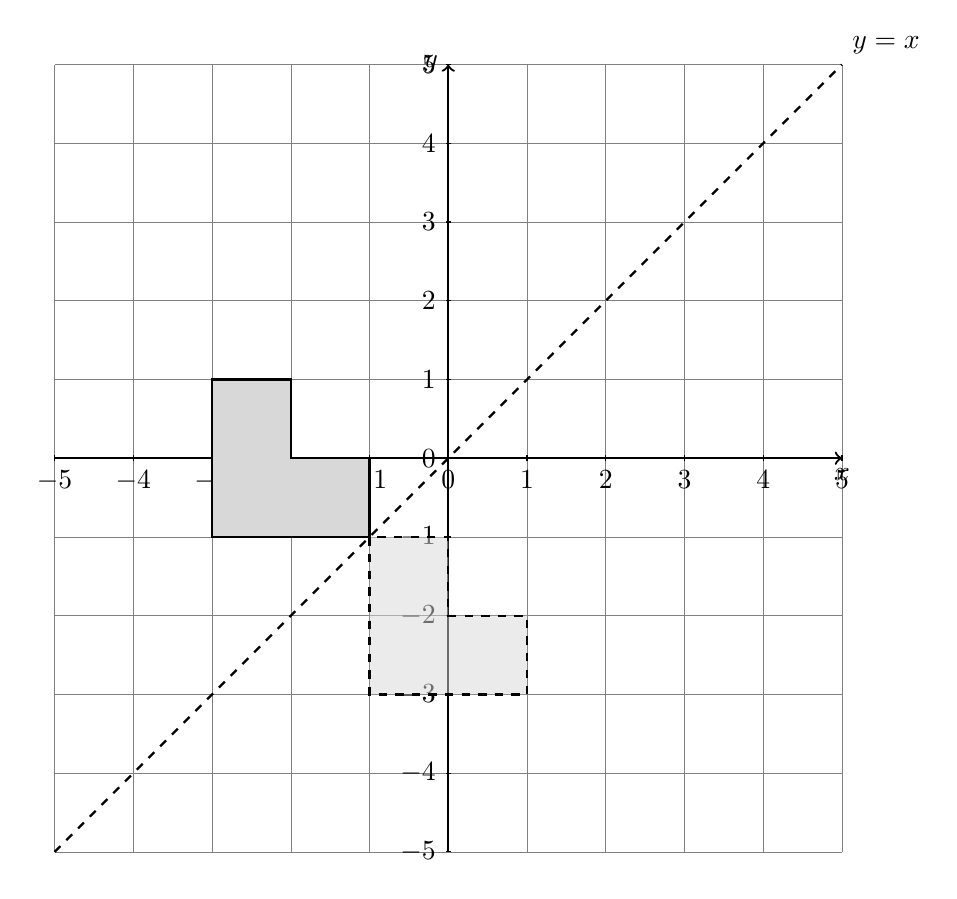
\begin{tikzpicture}[scale=1, transform shape]
    % Define colours
    \definecolor{borderColour}{HTML}{000000}
    \definecolor{fillColour}{HTML}{D8D8D8}
    
    % Define axis scale
    \def\axisLimit{5}

    % Draw grid
    \draw[step=1cm,gray,very thin] (-\axisLimit,-\axisLimit) grid (\axisLimit,\axisLimit);
    
    % Draw axes
    \draw[thick,->] (-5,0) -- (5,0) node[anchor=north] {$x$};
    \draw[thick,->] (0,-5) -- (0,5) node[anchor=east] {$y$};

    % Label x-axis and y-axis
    \foreach \x in {-\axisLimit,...,\axisLimit}
        \draw (\x cm,1pt) -- (\x cm,-1pt) node[anchor=north] {$\x$};
    \foreach \y in {-\axisLimit,...,\axisLimit}
        \draw (1pt,\y cm) -- (-1pt,\y cm) node[anchor=east] {$\y$};

    % Draw the reflection line y = x
    \draw[thick,dashed] (-5,-5) -- (5,5) node[anchor=south west] {$y=x$};

    % Define coordinates for the "L" shape
    \coordinate (A) at (-3,1);
    \coordinate (B) at (-2,1);
    \coordinate (C) at (-2,0);
    \coordinate (D) at (-3,0);
    \coordinate (E) at (-3,-1);
    \coordinate (F) at (-1,-1);
    \coordinate (G) at (-1,0);

    % Draw the original "L" shape and fill with light blue
    \filldraw[fill=fillColour, draw=borderColour, thick] (A) -- (B) -- (C) -- (G) -- (F) -- (E) -- cycle;

    % Calculate reflected coordinates
    \coordinate (A') at (1,-3);
    \coordinate (B') at (1,-2);
    \coordinate (C') at (0,-2);
    \coordinate (D') at (0,-3);
    \coordinate (E') at (-1,-3);
    \coordinate (F') at (-1,-1);
    \coordinate (G') at (0,-1);

    % Draw the reflected "L" shape and fill with light blue
    \filldraw[fill=fillColour, fill opacity=0.5, draw=borderColour, thick, dashed] (A') -- (B') -- (C') -- (G') -- (F') -- (E') -- cycle;
    
\end{tikzpicture}

% Q10
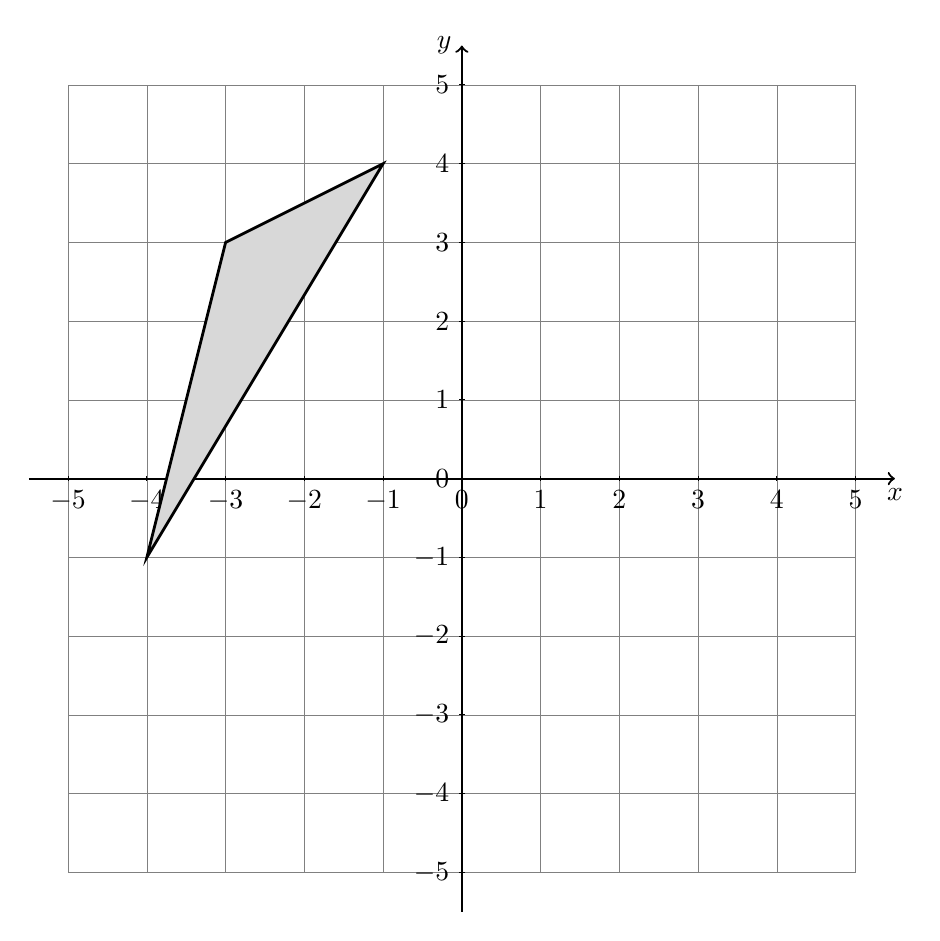
\begin{tikzpicture}[scale=1, transform shape]
    % Define colours
    \definecolor{borderColour}{HTML}{000000}
    \definecolor{fillColour}{HTML}{D8D8D8}
    
    % Define axis scale
    \def\axisLimit{5}

    % Draw grid
    \draw[step=1cm,gray,very thin] (-\axisLimit,-\axisLimit) grid (\axisLimit,\axisLimit);
    
    % Draw axes
    \draw[thick,->] (-\axisLimit-0.5,0) -- (\axisLimit+0.5,0) node[anchor=north] {$x$};
    \draw[thick,->] (0,-\axisLimit-0.5) -- (0,\axisLimit+0.5) node[anchor=east] {$y$};

    % Label x-axis and y-axis
    \foreach \x in {-\axisLimit,...,\axisLimit}
        \draw (\x cm,1pt) -- (\x cm,-1pt) node[anchor=north] {$\x$};
    \foreach \y in {-\axisLimit,...,\axisLimit}
        \draw (1pt,\y cm) -- (-1pt,\y cm) node[anchor=east] {$\y$};

    % Define coordinates for the triangle
    \coordinate (A) at (-3,3);
    \coordinate (B) at (-4,-1);
    \coordinate (C) at (-1,4);

    % Draw the triangle
    \filldraw[fillColour, draw=borderColour, line width=1pt] (A) -- (B) -- (C) -- cycle;

\end{tikzpicture}

% Q10 (solution)
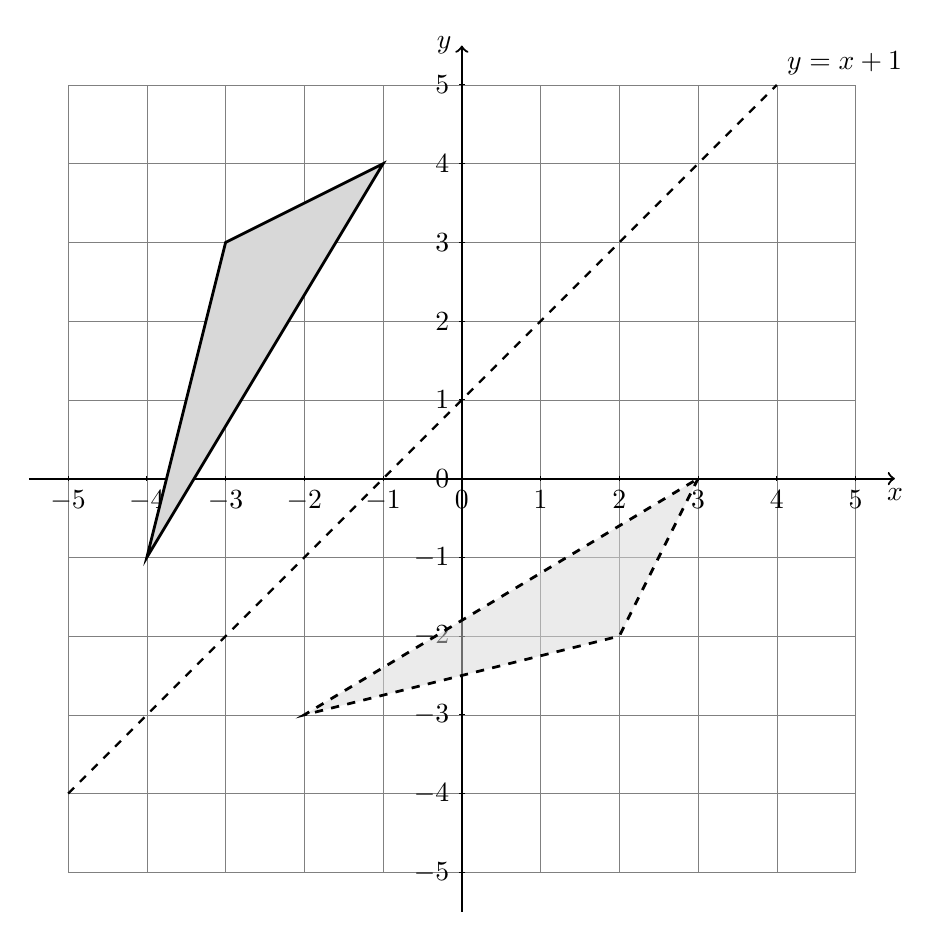
\begin{tikzpicture}[scale=1, transform shape]
    % Define colours
    \definecolor{borderColour}{HTML}{000000}
    \definecolor{fillColour}{HTML}{D8D8D8}
    
    % Define axis scale
    \def\axisLimit{5}

    % Draw grid
    \draw[step=1cm,gray,very thin] (-\axisLimit,-\axisLimit) grid (\axisLimit,\axisLimit);
    
    % Draw axes
    \draw[thick,->] (-\axisLimit-0.5,0) -- (\axisLimit+0.5,0) node[anchor=north] {$x$};
    \draw[thick,->] (0,-\axisLimit-0.5) -- (0,\axisLimit+0.5) node[anchor=east] {$y$};

    % Label x-axis and y-axis
    \foreach \x in {-\axisLimit,...,\axisLimit}
        \draw (\x cm,1pt) -- (\x cm,-1pt) node[anchor=north] {$\x$};
    \foreach \y in {-\axisLimit,...,\axisLimit}
        \draw (1pt,\y cm) -- (-1pt,\y cm) node[anchor=east] {$\y$};

    % Draw the reflection line y = x
    \draw[thick,dashed] (-5,-4) -- (4,5) node[anchor=south west] {$y=x+1$};

    % Define coordinates for the triangle
    \coordinate (A) at (-3,3);
    \coordinate (B) at (-4,-1);
    \coordinate (C) at (-1,4);

    % Draw the triangle
    \filldraw[fillColour, draw=borderColour, line width=1pt] (A) -- (B) -- (C) -- cycle;

    % Define coordinates for the transformed triangle
    \coordinate (D) at (3,0);
    \coordinate (E) at (2,-2);
    \coordinate (F) at (-2,-3);

    % Draw the transformed triangle
    \filldraw[fillColour, draw=borderColour, line width=1pt, dashed, fill opacity=0.5] (D) -- (E) -- (F) -- cycle;

\end{tikzpicture}

% Q11
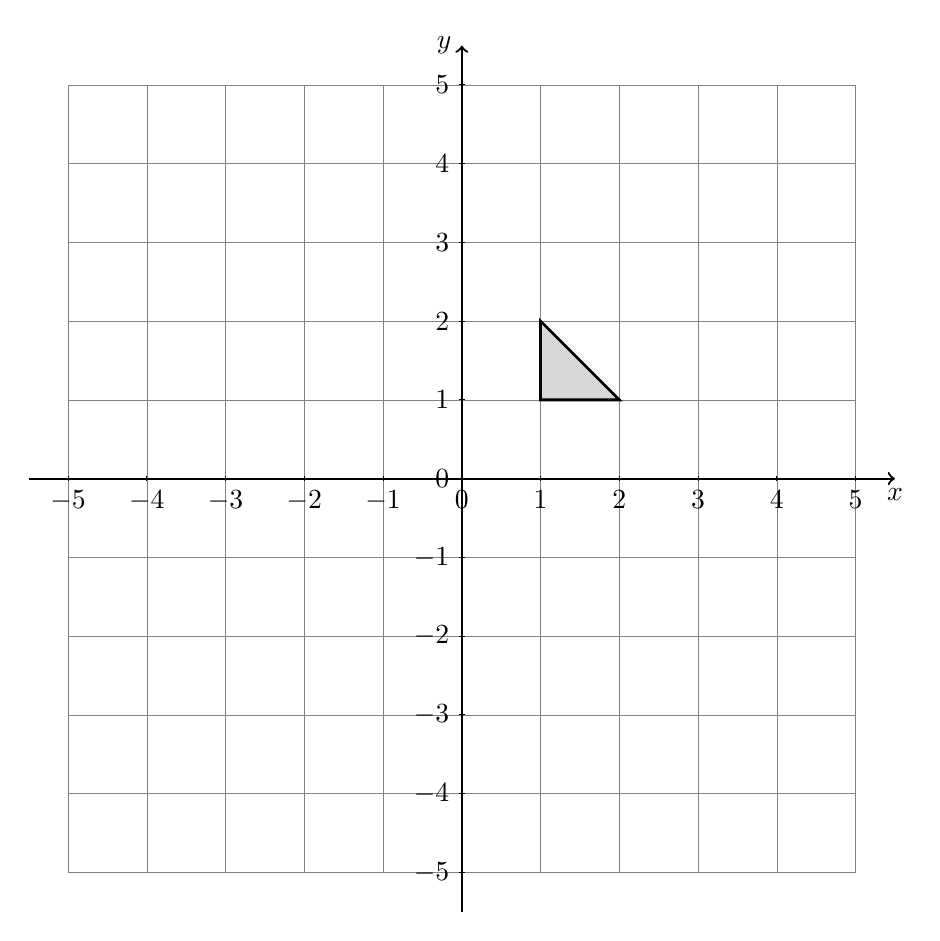
\begin{tikzpicture}[scale=1, transform shape]
    % Define axis scale
    \def\axisLimit{5}

    \definecolor{borderColour}{HTML}{000000}
    \definecolor{fillColour}{HTML}{D8D8D8}

    % Draw grid
    \draw[step=1cm,gray,very thin] (-\axisLimit,-\axisLimit) grid (\axisLimit,\axisLimit);
    
    % Draw axes
    \draw[thick,->] (-\axisLimit-0.5,0) -- (\axisLimit+0.5,0) node[anchor=north] {$x$};
    \draw[thick,->] (0,-\axisLimit-0.5) -- (0,\axisLimit+0.5) node[anchor=east] {$y$};

    % Label x-axis and y-axis
    \foreach \x in {-\axisLimit,...,\axisLimit}
        \draw (\x cm,1pt) -- (\x cm,-1pt) node[anchor=north] {$\x$};
    \foreach \y in {-\axisLimit,...,\axisLimit}
        \draw (1pt,\y cm) -- (-1pt,\y cm) node[anchor=east] {$\y$};

    % Define the center of rotation
    \coordinate (center) at (0,0);

    % Define coordinates for the original right-angled triangle
    \coordinate (A) at (1,1);
    \coordinate (B) at (1,2);
    \coordinate (C) at (2,1);

    % Draw the original right-angled triangle
    \filldraw[fill=fillColour, draw=borderColour, line width=1pt] (A) -- (B) -- (C) -- cycle;

\end{tikzpicture}

% Q11 (solution (i))
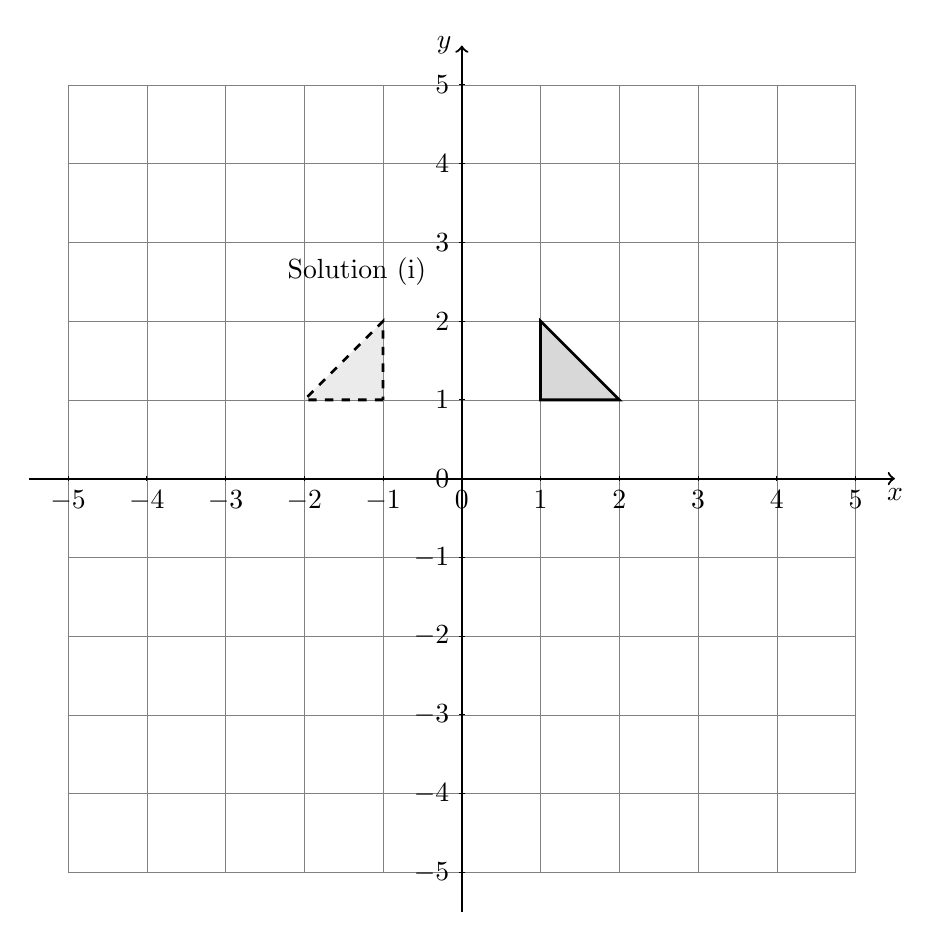
\begin{tikzpicture}[scale=1, transform shape]
    % Define axis scale
    \def\axisLimit{5}

    \definecolor{borderColour}{HTML}{000000}
    \definecolor{fillColour}{HTML}{D8D8D8}

    % Draw grid
    \draw[step=1cm,gray,very thin] (-\axisLimit,-\axisLimit) grid (\axisLimit,\axisLimit);
    
    % Draw axes
    \draw[thick,->] (-\axisLimit-0.5,0) -- (\axisLimit+0.5,0) node[anchor=north] {$x$};
    \draw[thick,->] (0,-\axisLimit-0.5) -- (0,\axisLimit+0.5) node[anchor=east] {$y$};

    % Label x-axis and y-axis
    \foreach \x in {-\axisLimit,...,\axisLimit}
        \draw (\x cm,1pt) -- (\x cm,-1pt) node[anchor=north] {$\x$};
    \foreach \y in {-\axisLimit,...,\axisLimit}
        \draw (1pt,\y cm) -- (-1pt,\y cm) node[anchor=east] {$\y$};

    % Define the center of rotation
    \coordinate (center) at (0,0);

    % Define coordinates for the original right-angled triangle
    \coordinate (A) at (1,1);
    \coordinate (B) at (1,2);
    \coordinate (C) at (2,1);

    % Draw the original right-angled triangle
    \filldraw[fill=fillColour, draw=borderColour, line width=1pt] (A) -- (B) -- (C) -- cycle;

    % Rotate around the defined center
    \coordinate (D) at ([rotate around={90:(center)}]A);
    \coordinate (E) at ([rotate around={90:(center)}]B);
    \coordinate (F) at ([rotate around={90:(center)}]C);

    % Draw the rotated triangles with 50% opacity
    \filldraw[fill=fillColour, draw=borderColour, line width=1pt, dashed, fill opacity=0.5] (D) -- (E) -- (F) -- cycle;
    \node at (barycentric cs:D=1,E=1,F=1) [above, yshift=1cm] {Solution (i)};

\end{tikzpicture}

% Q11 (solution (ii))
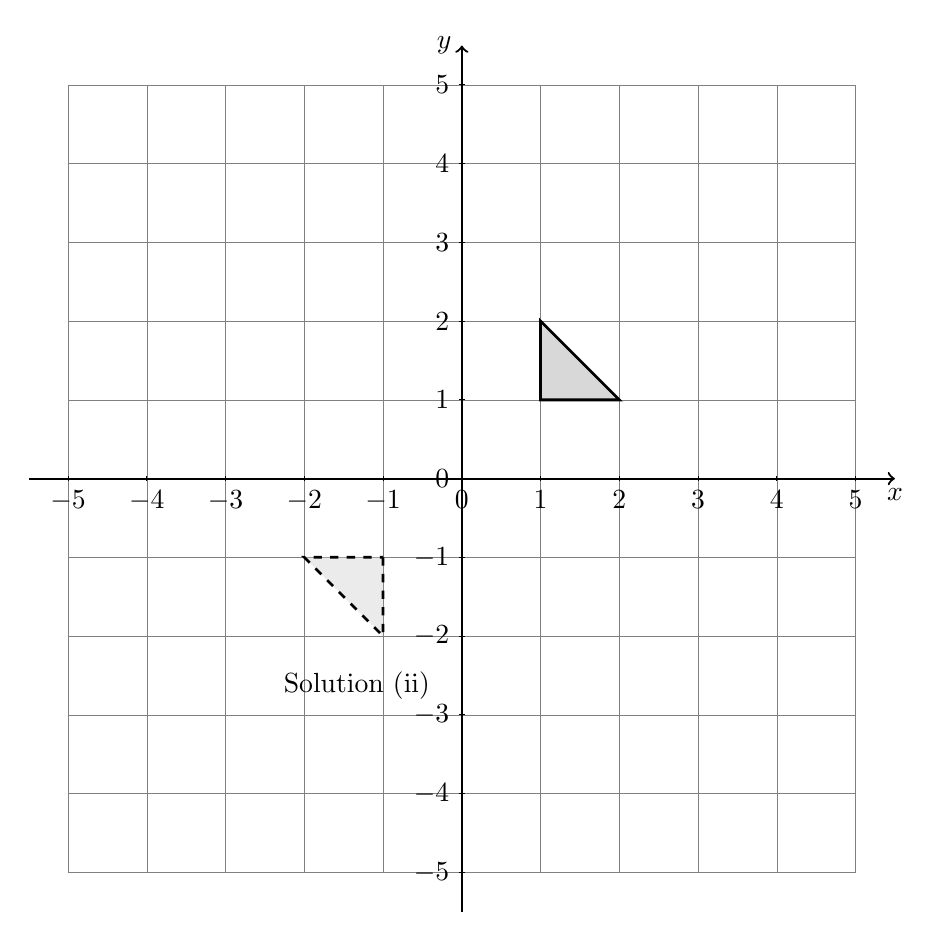
\begin{tikzpicture}[scale=1, transform shape]
    % Define axis scale
    \def\axisLimit{5}

    \definecolor{borderColour}{HTML}{000000}
    \definecolor{fillColour}{HTML}{D8D8D8}

    % Draw grid
    \draw[step=1cm,gray,very thin] (-\axisLimit,-\axisLimit) grid (\axisLimit,\axisLimit);
    
    % Draw axes
    \draw[thick,->] (-\axisLimit-0.5,0) -- (\axisLimit+0.5,0) node[anchor=north] {$x$};
    \draw[thick,->] (0,-\axisLimit-0.5) -- (0,\axisLimit+0.5) node[anchor=east] {$y$};

    % Label x-axis and y-axis
    \foreach \x in {-\axisLimit,...,\axisLimit}
        \draw (\x cm,1pt) -- (\x cm,-1pt) node[anchor=north] {$\x$};
    \foreach \y in {-\axisLimit,...,\axisLimit}
        \draw (1pt,\y cm) -- (-1pt,\y cm) node[anchor=east] {$\y$};

    % Define the center of rotation
    \coordinate (center) at (0,0);

    % Define coordinates for the original right-angled triangle
    \coordinate (A) at (1,1);
    \coordinate (B) at (1,2);
    \coordinate (C) at (2,1);

    % Draw the original right-angled triangle
    \filldraw[fill=fillColour, draw=borderColour, line width=1pt] (A) -- (B) -- (C) -- cycle;

    % Rotate around the defined center
    \coordinate (G) at ([rotate around={180:(center)}]A);
    \coordinate (H) at ([rotate around={180:(center)}]B);
    \coordinate (I) at ([rotate around={180:(center)}]C);

    % Draw the rotated triangles with 50% opacity
    \filldraw[fill=fillColour, draw=borderColour, line width=1pt, dashed, fill opacity=0.5] (G) -- (H) -- (I) -- cycle;
    \node at (barycentric cs:G=1,H=1,I=1) [below, yshift=-1cm] {Solution (ii)};

\end{tikzpicture}

% Q11 (solution (iii))
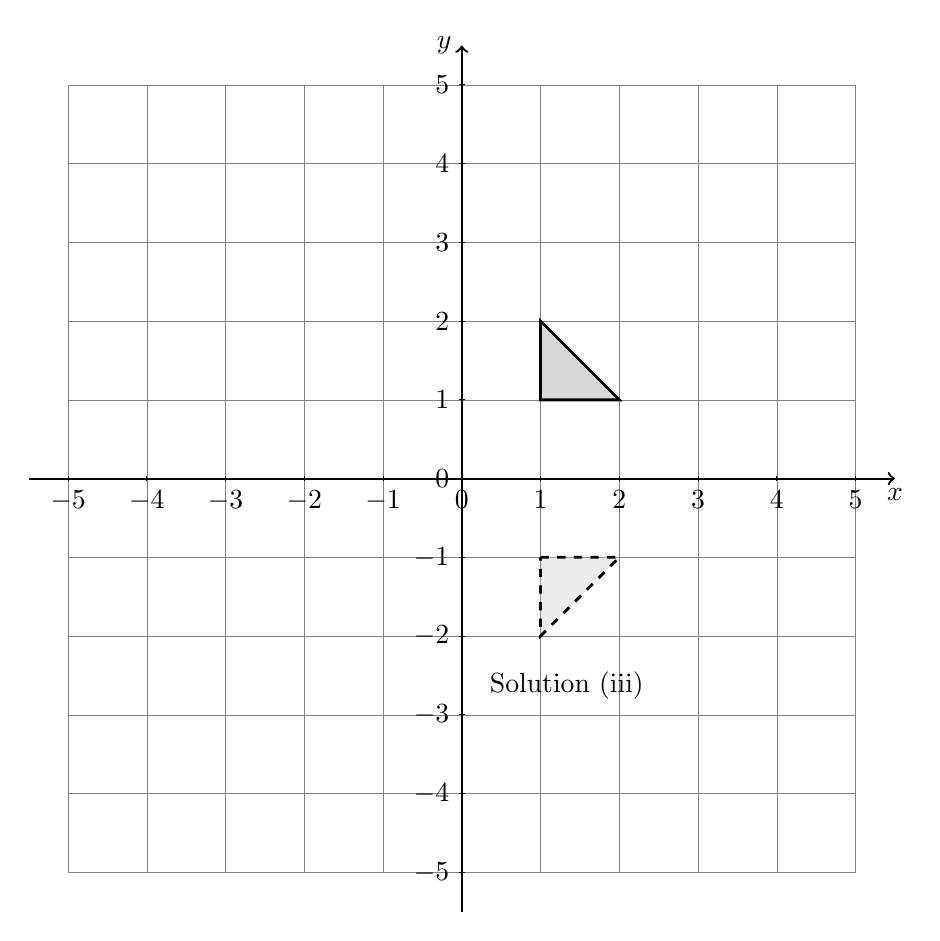
\begin{tikzpicture}[scale=1, transform shape]
    % Define axis scale
    \def\axisLimit{5}

    \definecolor{borderColour}{HTML}{000000}
    \definecolor{fillColour}{HTML}{D8D8D8}

    % Draw grid
    \draw[step=1cm,gray,very thin] (-\axisLimit,-\axisLimit) grid (\axisLimit,\axisLimit);
    
    % Draw axes
    \draw[thick,->] (-\axisLimit-0.5,0) -- (\axisLimit+0.5,0) node[anchor=north] {$x$};
    \draw[thick,->] (0,-\axisLimit-0.5) -- (0,\axisLimit+0.5) node[anchor=east] {$y$};

    % Label x-axis and y-axis
    \foreach \x in {-\axisLimit,...,\axisLimit}
        \draw (\x cm,1pt) -- (\x cm,-1pt) node[anchor=north] {$\x$};
    \foreach \y in {-\axisLimit,...,\axisLimit}
        \draw (1pt,\y cm) -- (-1pt,\y cm) node[anchor=east] {$\y$};

    % Define the center of rotation
    \coordinate (center) at (0,0);

    % Define coordinates for the original right-angled triangle
    \coordinate (A) at (1,1);
    \coordinate (B) at (1,2);
    \coordinate (C) at (2,1);

    % Draw the original right-angled triangle
    \filldraw[fill=fillColour, draw=borderColour, line width=1pt] (A) -- (B) -- (C) -- cycle;

    % Rotate around the defined center
    \coordinate (J) at ([rotate around={270:(center)}]A);
    \coordinate (K) at ([rotate around={270:(center)}]B);
    \coordinate (L) at ([rotate around={270:(center)}]C);

    % Draw the rotated triangles with 50% opacity
    \filldraw[fill=fillColour, draw=borderColour, line width=1pt, dashed, fill opacity=0.5] (J) -- (K) -- (L) -- cycle;
    \node at (barycentric cs:J=1,K=1,L=1) [below, yshift=-1cm] {Solution (iii)};

\end{tikzpicture}

% Q12
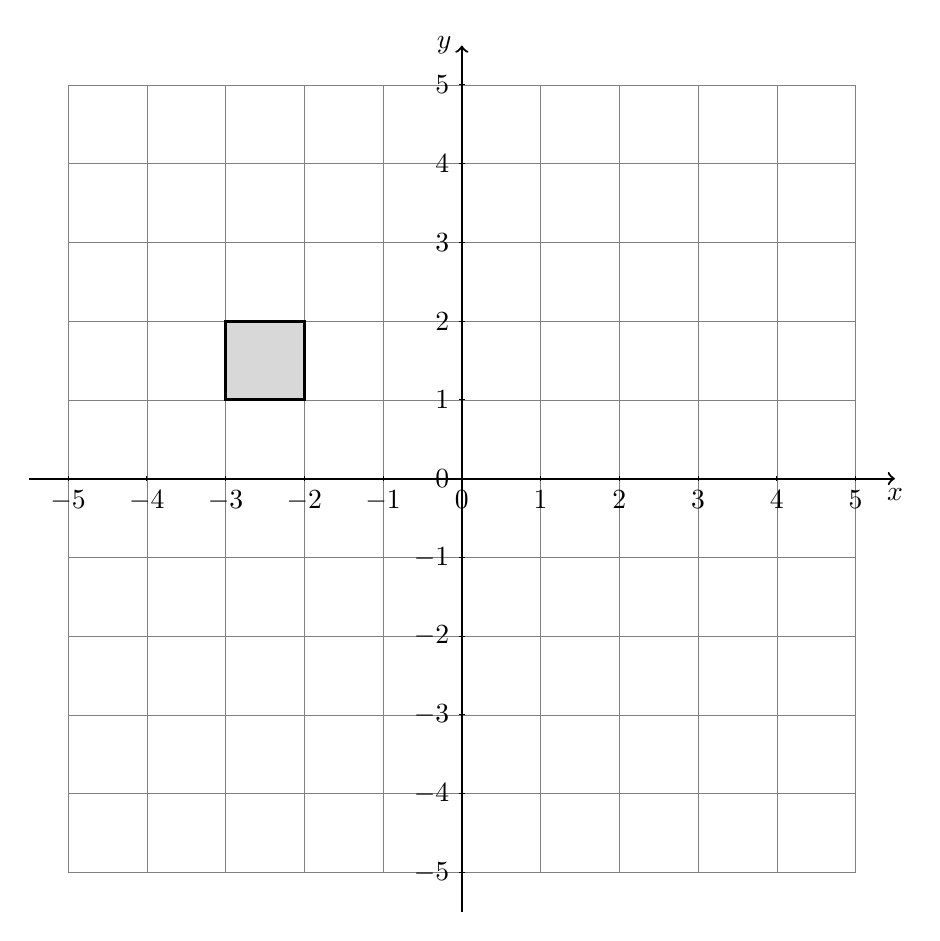
\begin{tikzpicture}[scale=1, transform shape]
    % Define axis scale
    \def\axisLimit{5}

    \definecolor{borderColour}{HTML}{000000}
    \definecolor{fillColour}{HTML}{D8D8D8}

    % Draw grid
    \draw[step=1cm,gray,very thin] (-\axisLimit,-\axisLimit) grid (\axisLimit,\axisLimit);
    
    % Draw axes
    \draw[thick,->] (-\axisLimit-0.5,0) -- (\axisLimit+0.5,0) node[anchor=north] {$x$};
    \draw[thick,->] (0,-\axisLimit-0.5) -- (0,\axisLimit+0.5) node[anchor=east] {$y$};

    % Label x-axis and y-axis
    \foreach \x in {-\axisLimit,...,\axisLimit}
        \draw (\x cm,1pt) -- (\x cm,-1pt) node[anchor=north] {$\x$};
    \foreach \y in {-\axisLimit,...,\axisLimit}
        \draw (1pt,\y cm) -- (-1pt,\y cm) node[anchor=east] {$\y$};

    % Define the center of rotation
    \coordinate (center) at (0,0);

    % Define coordinates for the original right-angled triangle
    \coordinate (A) at (-3,2);
    \coordinate (B) at (-2,2);
    \coordinate (C) at (-2,1);
    \coordinate (D) at (-3,1);
    
    % Draw the original right-angled triangle
    \filldraw[fill=fillColour, draw=borderColour, line width=1pt] (A) -- (B) -- (C) -- (D) -- cycle;
    
\end{tikzpicture}

% Q12 (solution (i))
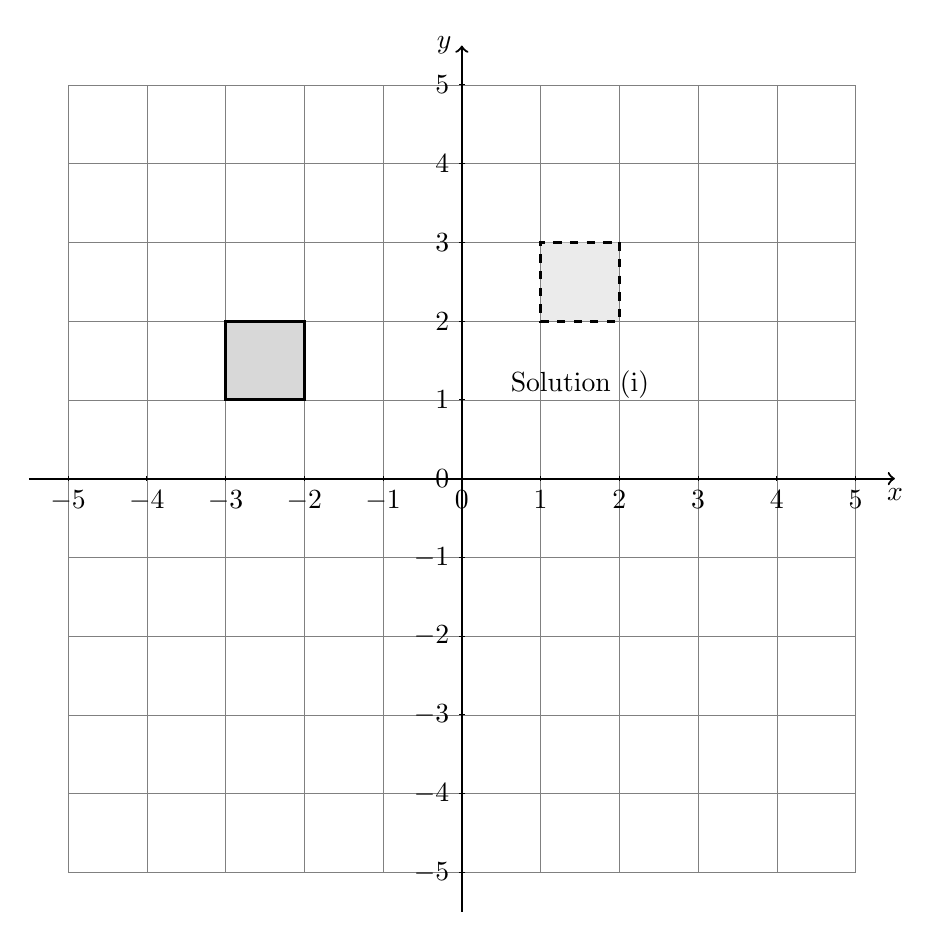
\begin{tikzpicture}[scale=1, transform shape]
    % Define axis scale
    \def\axisLimit{5}

    \definecolor{borderColour}{HTML}{000000}
    \definecolor{fillColour}{HTML}{D8D8D8}

    % Draw grid
    \draw[step=1cm,gray,very thin] (-\axisLimit,-\axisLimit) grid (\axisLimit,\axisLimit);
    
    % Draw axes
    \draw[thick,->] (-\axisLimit-0.5,0) -- (\axisLimit+0.5,0) node[anchor=north] {$x$};
    \draw[thick,->] (0,-\axisLimit-0.5) -- (0,\axisLimit+0.5) node[anchor=east] {$y$};

    % Label x-axis and y-axis
    \foreach \x in {-\axisLimit,...,\axisLimit}
        \draw (\x cm,1pt) -- (\x cm,-1pt) node[anchor=north] {$\x$};
    \foreach \y in {-\axisLimit,...,\axisLimit}
        \draw (1pt,\y cm) -- (-1pt,\y cm) node[anchor=east] {$\y$};

    % Define the center of rotation
    \coordinate (center) at (0,0);

    % Define coordinates for the original right-angled triangle
    \coordinate (A) at (-3,2);
    \coordinate (B) at (-2,2);
    \coordinate (C) at (-2,1);
    \coordinate (D) at (-3,1);
    
    % Draw the original right-angled triangle
    \filldraw[fill=fillColour, draw=borderColour, line width=1pt] (A) -- (B) -- (C) -- (D) -- cycle;

    % Rotate around the defined center
    \coordinate (M) at ([rotate around={270:(center)}]A);
    \coordinate (N) at ([rotate around={270:(center)}]B);
    \coordinate (O) at ([rotate around={270:(center)}]C);
    \coordinate (P) at ([rotate around={270:(center)}]D);

    % Draw the rotated triangle with 50% opacity
    \filldraw[fill=fillColour, draw=borderColour, line width=1pt, dashed, fill opacity=0.5] (M) -- (N) -- (O) -- (P) -- cycle;
    \node at (barycentric cs:M=1,N=1,O=1,P=1) [below, yshift=-1cm] {Solution (i)};

\end{tikzpicture}

% Q12 (solution (ii))
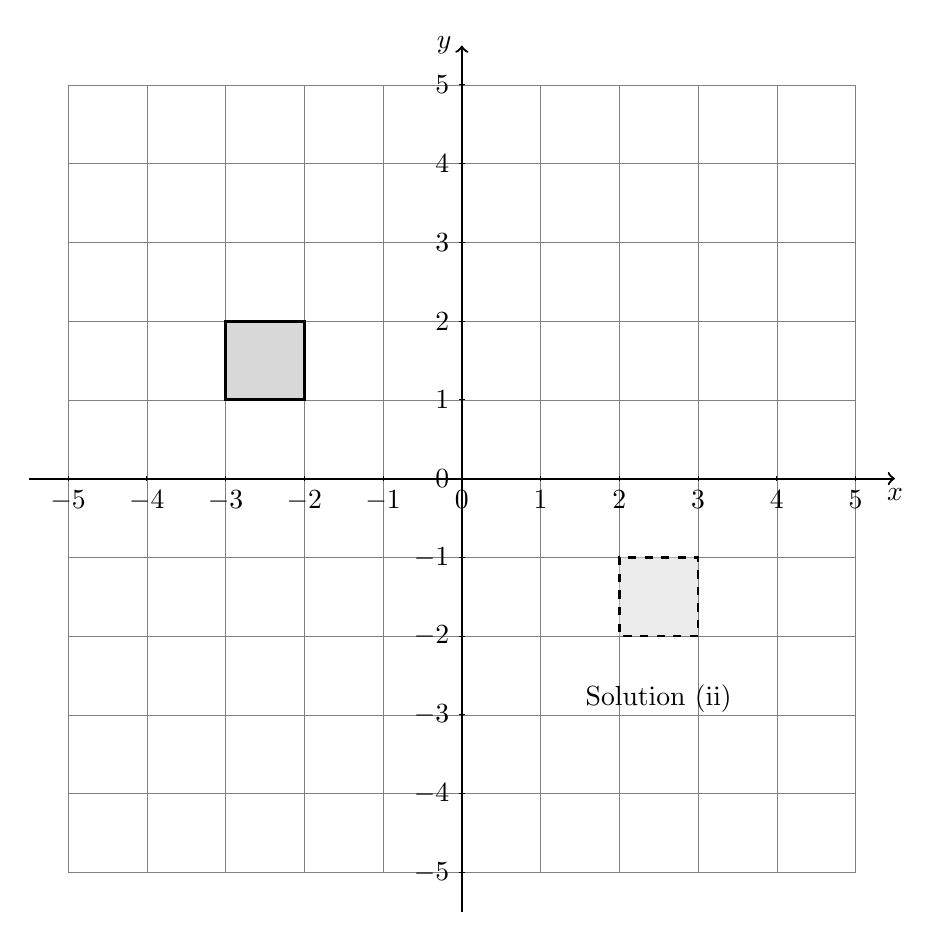
\begin{tikzpicture}[scale=1, transform shape]
    % Define axis scale
    \def\axisLimit{5}

    \definecolor{borderColour}{HTML}{000000}
    \definecolor{fillColour}{HTML}{D8D8D8}

    % Draw grid
    \draw[step=1cm,gray,very thin] (-\axisLimit,-\axisLimit) grid (\axisLimit,\axisLimit);
    
    % Draw axes
    \draw[thick,->] (-\axisLimit-0.5,0) -- (\axisLimit+0.5,0) node[anchor=north] {$x$};
    \draw[thick,->] (0,-\axisLimit-0.5) -- (0,\axisLimit+0.5) node[anchor=east] {$y$};

    % Label x-axis and y-axis
    \foreach \x in {-\axisLimit,...,\axisLimit}
        \draw (\x cm,1pt) -- (\x cm,-1pt) node[anchor=north] {$\x$};
    \foreach \y in {-\axisLimit,...,\axisLimit}
        \draw (1pt,\y cm) -- (-1pt,\y cm) node[anchor=east] {$\y$};

    % Define the center of rotation
    \coordinate (center) at (0,0);

    % Define coordinates for the original right-angled triangle
    \coordinate (A) at (-3,2);
    \coordinate (B) at (-2,2);
    \coordinate (C) at (-2,1);
    \coordinate (D) at (-3,1);
    
    % Draw the original right-angled triangle
    \filldraw[fill=fillColour, draw=borderColour, line width=1pt] (A) -- (B) -- (C) -- (D) -- cycle;

    % Rotate around the defined center
    \coordinate (I) at ([rotate around={180:(center)}]A);
    \coordinate (J) at ([rotate around={180:(center)}]B);
    \coordinate (K) at ([rotate around={180:(center)}]C);
    \coordinate (L) at ([rotate around={180:(center)}]D);
    % Draw the rotated triangle with 50% opacity
    \filldraw[fill=fillColour, draw=borderColour, line width=1pt, dashed, fill opacity=0.5] (I) -- (J) -- (K) -- (L) -- cycle;
    \node at (barycentric cs:I=1,J=1,K=1,L=1) [below, yshift=-1cm] {Solution (ii)};

\end{tikzpicture}

% Q12 (solution (iii))
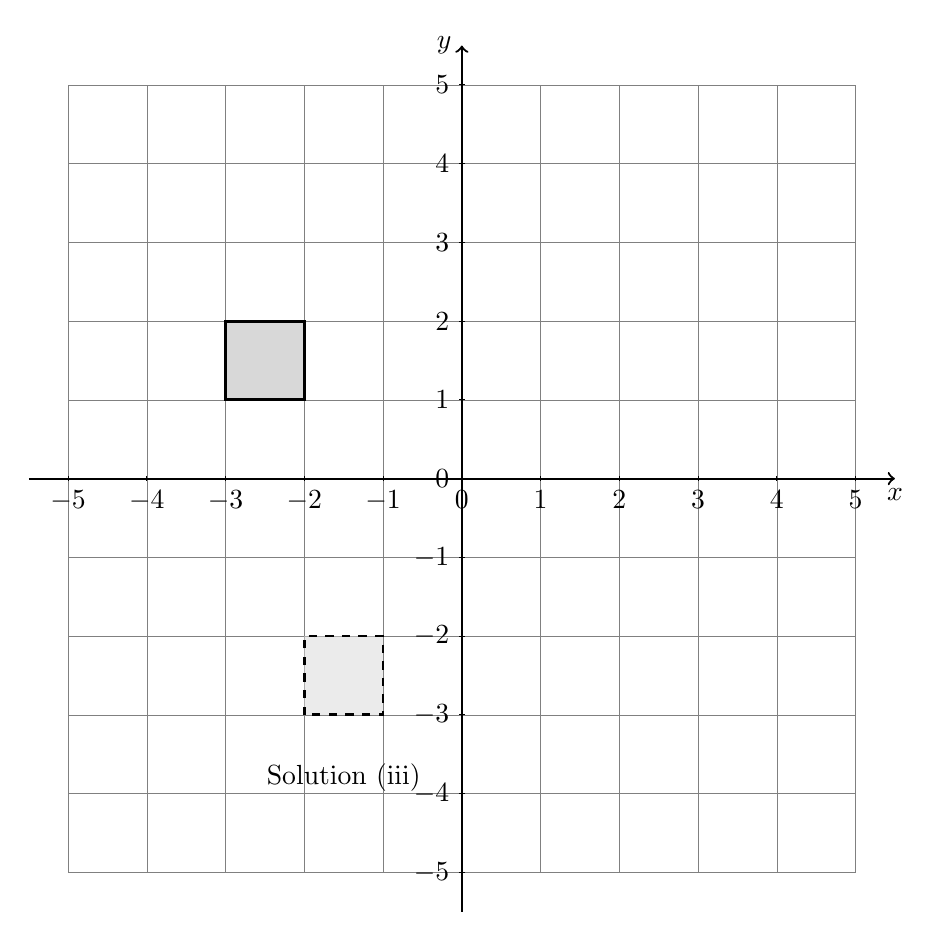
\begin{tikzpicture}[scale=1, transform shape]
    % Define axis scale
    \def\axisLimit{5}

    \definecolor{borderColour}{HTML}{000000}
    \definecolor{fillColour}{HTML}{D8D8D8}

    % Draw grid
    \draw[step=1cm,gray,very thin] (-\axisLimit,-\axisLimit) grid (\axisLimit,\axisLimit);
    
    % Draw axes
    \draw[thick,->] (-\axisLimit-0.5,0) -- (\axisLimit+0.5,0) node[anchor=north] {$x$};
    \draw[thick,->] (0,-\axisLimit-0.5) -- (0,\axisLimit+0.5) node[anchor=east] {$y$};

    % Label x-axis and y-axis
    \foreach \x in {-\axisLimit,...,\axisLimit}
        \draw (\x cm,1pt) -- (\x cm,-1pt) node[anchor=north] {$\x$};
    \foreach \y in {-\axisLimit,...,\axisLimit}
        \draw (1pt,\y cm) -- (-1pt,\y cm) node[anchor=east] {$\y$};

    % Define the center of rotation
    \coordinate (center) at (0,0);

    % Define coordinates for the original right-angled triangle
    \coordinate (A) at (-3,2);
    \coordinate (B) at (-2,2);
    \coordinate (C) at (-2,1);
    \coordinate (D) at (-3,1);
    
    % Draw the original right-angled triangle
    \filldraw[fill=fillColour, draw=borderColour, line width=1pt] (A) -- (B) -- (C) -- (D) -- cycle;

    % Rotate around the defined center
    \coordinate (E) at ([rotate around={90:(center)}]A);
    \coordinate (F) at ([rotate around={90:(center)}]B);
    \coordinate (G) at ([rotate around={90:(center)}]C);
    \coordinate (H) at ([rotate around={90:(center)}]D);

    % Draw the rotated triangle with 50% opacity
    \filldraw[fill=fillColour, draw=borderColour, line width=1pt, dashed, fill opacity=0.5] (E) -- (F) -- (G) -- (H) -- cycle;
    \node at (barycentric cs:E=1,F=1,G=1,H=1) [below, yshift=-1cm] {Solution (iii)};

\end{tikzpicture}

% Q13
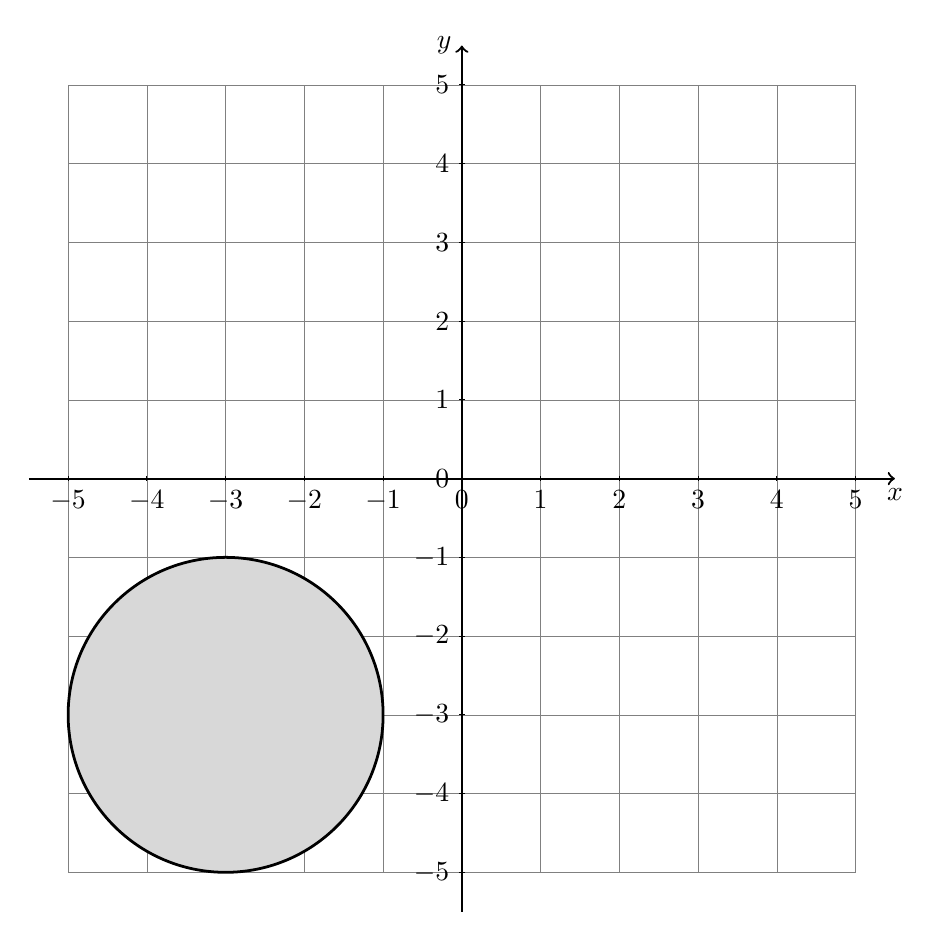
\begin{tikzpicture}[scale=1, transform shape]
    % Define axis scale
    \def\axisLimit{5}

    \definecolor{borderColour}{HTML}{000000}
    \definecolor{fillColour}{HTML}{D8D8D8}

    % Draw grid
    \draw[step=1cm,gray,very thin] (-\axisLimit,-\axisLimit) grid (\axisLimit,\axisLimit);
    
    % Draw axes
    \draw[thick,->] (-\axisLimit-0.5,0) -- (\axisLimit+0.5,0) node[anchor=north] {$x$};
    \draw[thick,->] (0,-\axisLimit-0.5) -- (0,\axisLimit+0.5) node[anchor=east] {$y$};

    % Label x-axis and y-axis
    \foreach \x in {-\axisLimit,...,\axisLimit}
        \draw (\x cm,1pt) -- (\x cm,-1pt) node[anchor=north] {$\x$};
    \foreach \y in {-\axisLimit,...,\axisLimit}
        \draw (1pt,\y cm) -- (-1pt,\y cm) node[anchor=east] {$\y$};

    % Define the center of rotation
    \coordinate (center) at (0,0);

    % Define the center for the original circle
    \coordinate (originalCenter) at (-3,-3);

    % Draw the original circle
    \draw[fill=fillColour, draw=borderColour, line width=1pt] (originalCenter) circle (2cm);

\end{tikzpicture}

% Q13 (solution (i))
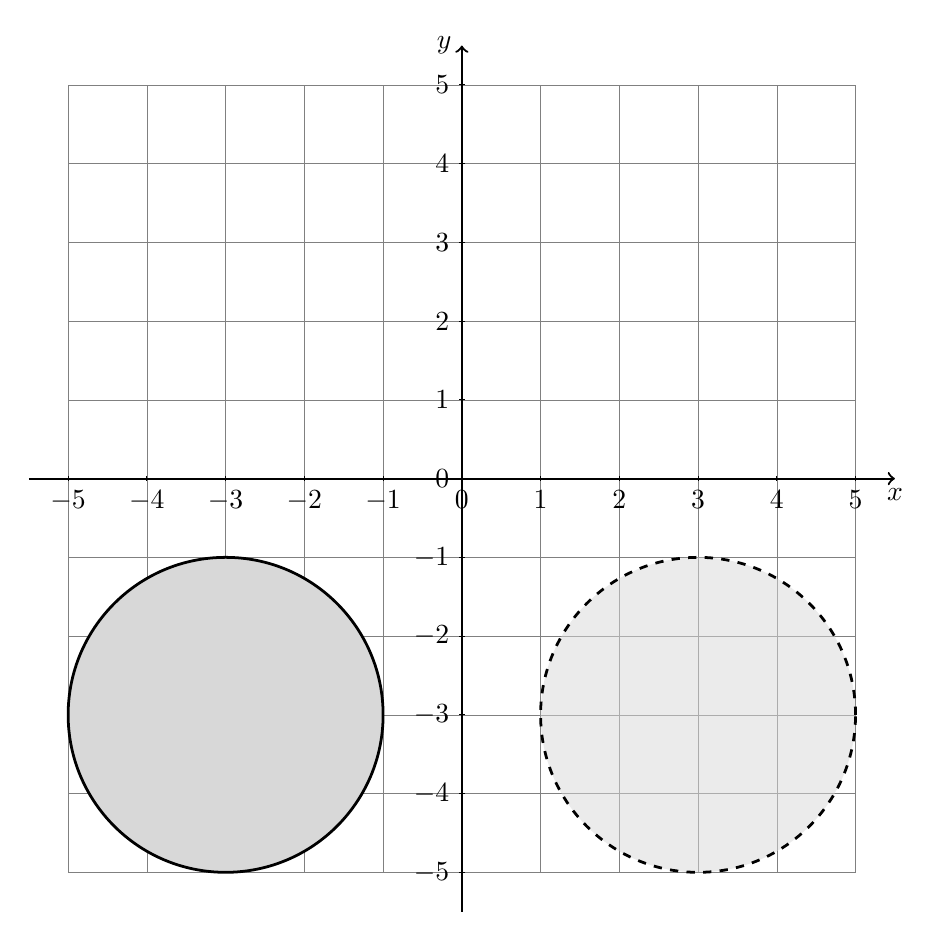
\begin{tikzpicture}[scale=1, transform shape]
    % Define axis scale
    \def\axisLimit{5}

    \definecolor{borderColour}{HTML}{000000}
    \definecolor{fillColour}{HTML}{D8D8D8}

    % Draw grid
    \draw[step=1cm,gray,very thin] (-\axisLimit,-\axisLimit) grid (\axisLimit,\axisLimit);
    
    % Draw axes
    \draw[thick,->] (-\axisLimit-0.5,0) -- (\axisLimit+0.5,0) node[anchor=north] {$x$};
    \draw[thick,->] (0,-\axisLimit-0.5) -- (0,\axisLimit+0.5) node[anchor=east] {$y$};

    % Label x-axis and y-axis
    \foreach \x in {-\axisLimit,...,\axisLimit}
        \draw (\x cm,1pt) -- (\x cm,-1pt) node[anchor=north] {$\x$};
    \foreach \y in {-\axisLimit,...,\axisLimit}
        \draw (1pt,\y cm) -- (-1pt,\y cm) node[anchor=east] {$\y$};

    % Define the center of rotation
    \coordinate (center) at (0,0);

    % Define the center for the original circle
    \coordinate (originalCenter) at (-3,-3);

    % Draw the original circle
    \draw[fill=fillColour, draw=borderColour, line width=1pt] (originalCenter) circle (2cm);

    % Calculate the new centers after rotation
    \coordinate (center90) at ([rotate around={90:(center)}]originalCenter);

    % Draw the rotated circles with 50% opacity
    \draw[fill=fillColour, draw=borderColour, line width=1pt, dashed, fill opacity=0.5] (center90) circle (2cm);

\end{tikzpicture}

% Q13 (solution (ii))
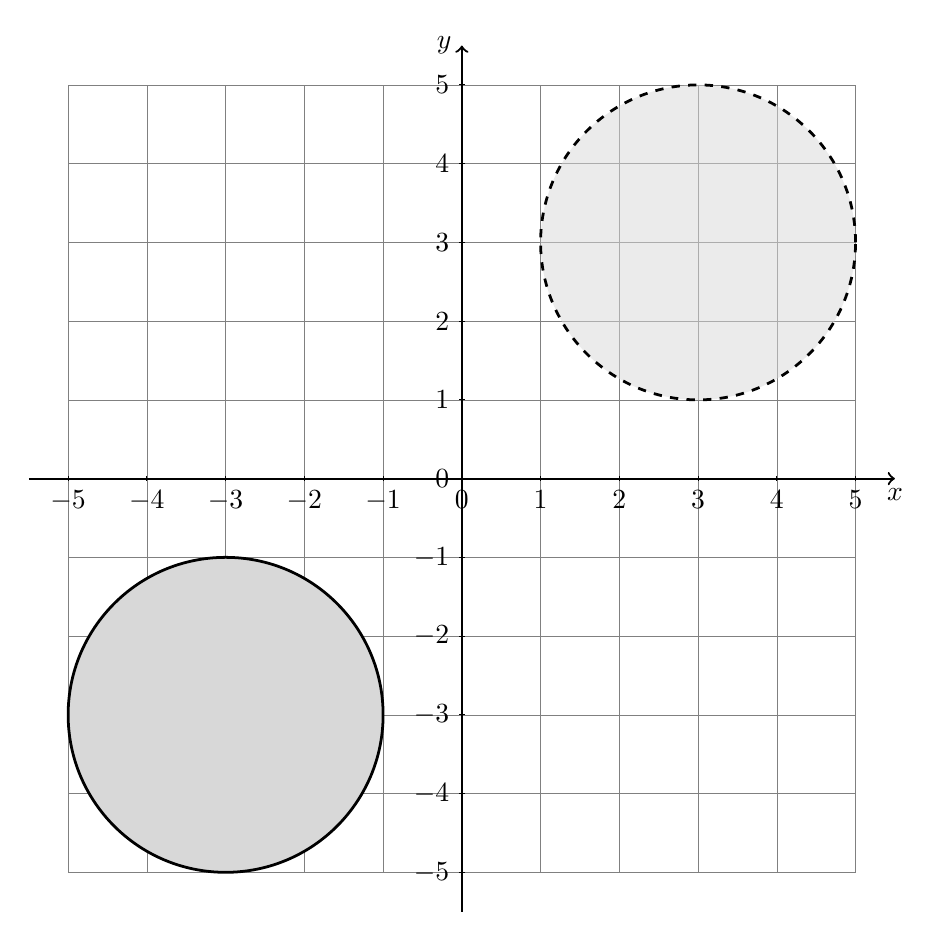
\begin{tikzpicture}[scale=1, transform shape]
    % Define axis scale
    \def\axisLimit{5}

    \definecolor{borderColour}{HTML}{000000}
    \definecolor{fillColour}{HTML}{D8D8D8}

    % Draw grid
    \draw[step=1cm,gray,very thin] (-\axisLimit,-\axisLimit) grid (\axisLimit,\axisLimit);
    
    % Draw axes
    \draw[thick,->] (-\axisLimit-0.5,0) -- (\axisLimit+0.5,0) node[anchor=north] {$x$};
    \draw[thick,->] (0,-\axisLimit-0.5) -- (0,\axisLimit+0.5) node[anchor=east] {$y$};

    % Label x-axis and y-axis
    \foreach \x in {-\axisLimit,...,\axisLimit}
        \draw (\x cm,1pt) -- (\x cm,-1pt) node[anchor=north] {$\x$};
    \foreach \y in {-\axisLimit,...,\axisLimit}
        \draw (1pt,\y cm) -- (-1pt,\y cm) node[anchor=east] {$\y$};

    % Define the center of rotation
    \coordinate (center) at (0,0);

    % Define the center for the original circle
    \coordinate (originalCenter) at (-3,-3);

    % Draw the original circle
    \draw[fill=fillColour, draw=borderColour, line width=1pt] (originalCenter) circle (2cm);

    % Calculate the new centers after rotation
    \coordinate (center180) at ([rotate around={180:(center)}]originalCenter);

    % Draw the rotated circles with 50% opacity
    \draw[fill=fillColour, draw=borderColour, line width=1pt, dashed, fill opacity=0.5] (center180) circle (2cm);

\end{tikzpicture}

% Q13 (solution (iii))
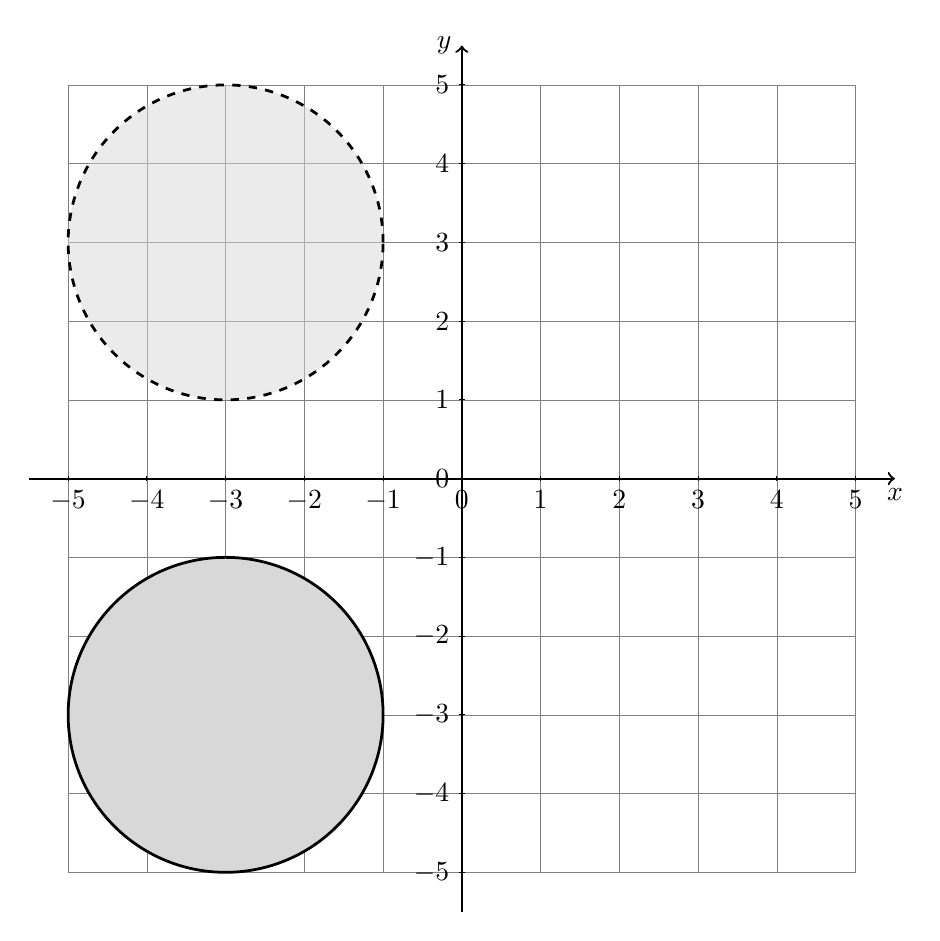
\begin{tikzpicture}[scale=1, transform shape]
    % Define axis scale
    \def\axisLimit{5}

    \definecolor{borderColour}{HTML}{000000}
    \definecolor{fillColour}{HTML}{D8D8D8}

    % Draw grid
    \draw[step=1cm,gray,very thin] (-\axisLimit,-\axisLimit) grid (\axisLimit,\axisLimit);
    
    % Draw axes
    \draw[thick,->] (-\axisLimit-0.5,0) -- (\axisLimit+0.5,0) node[anchor=north] {$x$};
    \draw[thick,->] (0,-\axisLimit-0.5) -- (0,\axisLimit+0.5) node[anchor=east] {$y$};

    % Label x-axis and y-axis
    \foreach \x in {-\axisLimit,...,\axisLimit}
        \draw (\x cm,1pt) -- (\x cm,-1pt) node[anchor=north] {$\x$};
    \foreach \y in {-\axisLimit,...,\axisLimit}
        \draw (1pt,\y cm) -- (-1pt,\y cm) node[anchor=east] {$\y$};

    % Define the center of rotation
    \coordinate (center) at (0,0);

    % Define the center for the original circle
    \coordinate (originalCenter) at (-3,-3);

    % Draw the original circle
    \draw[fill=fillColour, draw=borderColour, line width=1pt] (originalCenter) circle (2cm);

    % Calculate the new centers after rotation
    \coordinate (center270) at ([rotate around={270:(center)}]originalCenter);

    % Draw the rotated circles with 50% opacity
    \draw[fill=fillColour, draw=borderColour, line width=1pt, dashed, fill opacity=0.5] (center270) circle (2cm);

\end{tikzpicture}

% Q14
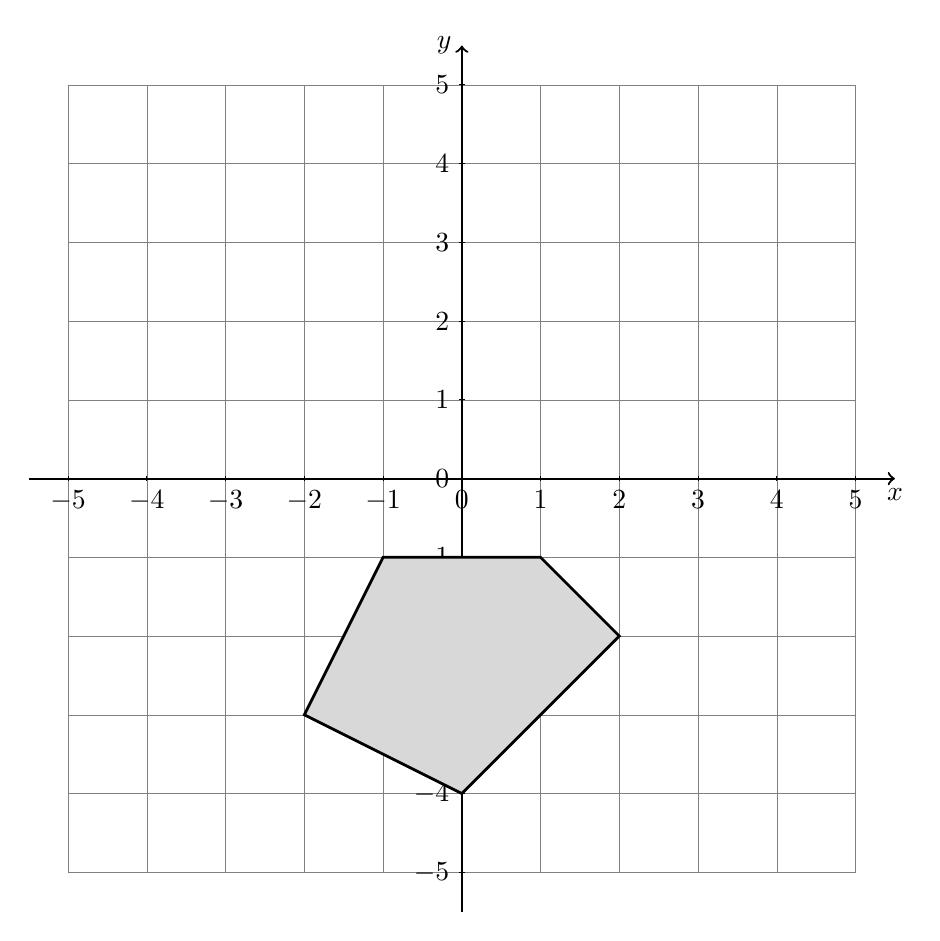
\begin{tikzpicture}[scale=1, transform shape]
    % Define axis scale
    \def\axisLimit{5}

    \definecolor{borderColour}{HTML}{000000}
    \definecolor{fillColour}{HTML}{D8D8D8}

    % Draw grid
    \draw[step=1cm,gray,very thin] (-\axisLimit,-\axisLimit) grid (\axisLimit,\axisLimit);
    
    % Draw axes
    \draw[thick,->] (-\axisLimit-0.5,0) -- (\axisLimit+0.5,0) node[anchor=north] {$x$};
    \draw[thick,->] (0,-\axisLimit-0.5) -- (0,\axisLimit+0.5) node[anchor=east] {$y$};

    % Label x-axis and y-axis
    \foreach \x in {-\axisLimit,...,\axisLimit}
        \draw (\x cm,1pt) -- (\x cm,-1pt) node[anchor=north] {$\x$};
    \foreach \y in {-\axisLimit,...,\axisLimit}
        \draw (1pt,\y cm) -- (-1pt,\y cm) node[anchor=east] {$\y$};

    % Define the center of rotation
    \coordinate (center) at (0,0);

    % Define the vertices for the original irregular polygon
    \coordinate (V1) at (-1,-1);
    \coordinate (V2) at (-2,-3);
    \coordinate (V3) at (0,-4);
    \coordinate (V4) at (2,-2);
    \coordinate (V5) at (1,-1);

    % Draw the original irregular polygon
    \draw[fill=fillColour, draw=borderColour, line width=1pt] (V1) -- (V2) -- (V3) -- (V4) -- (V5) -- cycle;

\end{tikzpicture}

% Q14 (solution (i))
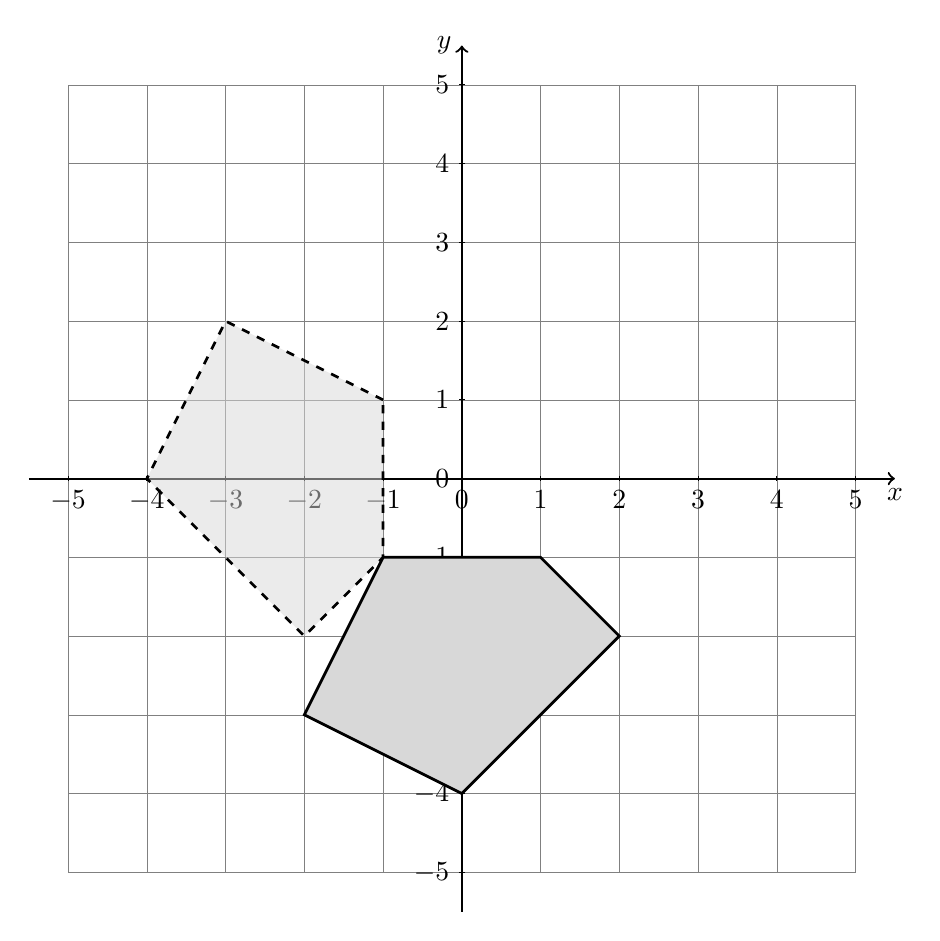
\begin{tikzpicture}[scale=1, transform shape]
    % Define axis scale
    \def\axisLimit{5}

    \definecolor{borderColour}{HTML}{000000}
    \definecolor{fillColour}{HTML}{D8D8D8}

    % Draw grid
    \draw[step=1cm,gray,very thin] (-\axisLimit,-\axisLimit) grid (\axisLimit,\axisLimit);
    
    % Draw axes
    \draw[thick,->] (-\axisLimit-0.5,0) -- (\axisLimit+0.5,0) node[anchor=north] {$x$};
    \draw[thick,->] (0,-\axisLimit-0.5) -- (0,\axisLimit+0.5) node[anchor=east] {$y$};

    % Label x-axis and y-axis
    \foreach \x in {-\axisLimit,...,\axisLimit}
        \draw (\x cm,1pt) -- (\x cm,-1pt) node[anchor=north] {$\x$};
    \foreach \y in {-\axisLimit,...,\axisLimit}
        \draw (1pt,\y cm) -- (-1pt,\y cm) node[anchor=east] {$\y$};

    % Define the center of rotation
    \coordinate (center) at (0,0);

    % Define the vertices for the original irregular polygon
    \coordinate (V1) at (-1,-1);
    \coordinate (V2) at (-2,-3);
    \coordinate (V3) at (0,-4);
    \coordinate (V4) at (2,-2);
    \coordinate (V5) at (1,-1);

    % Draw the original irregular polygon
    \draw[fill=fillColour, draw=borderColour, line width=1pt] (V1) -- (V2) -- (V3) -- (V4) -- (V5) -- cycle;

    % Calculate the new vertices after rotation
    \foreach \angle in {270} {
        \coordinate (V1\angle) at ([rotate around={\angle:(center)}]V1);
        \coordinate (V2\angle) at ([rotate around={\angle:(center)}]V2);
        \coordinate (V3\angle) at ([rotate around={\angle:(center)}]V3);
        \coordinate (V4\angle) at ([rotate around={\angle:(center)}]V4);
        \coordinate (V5\angle) at ([rotate around={\angle:(center)}]V5);
        % Draw the rotated polygon with 50% opacity
        \draw[fill=fillColour, draw=borderColour, line width=1pt, dashed, fill opacity=0.5] 
            (V1\angle) -- (V2\angle) -- (V3\angle) -- (V4\angle) -- (V5\angle) -- cycle;
    }

\end{tikzpicture}

% Q14 (solution (ii))
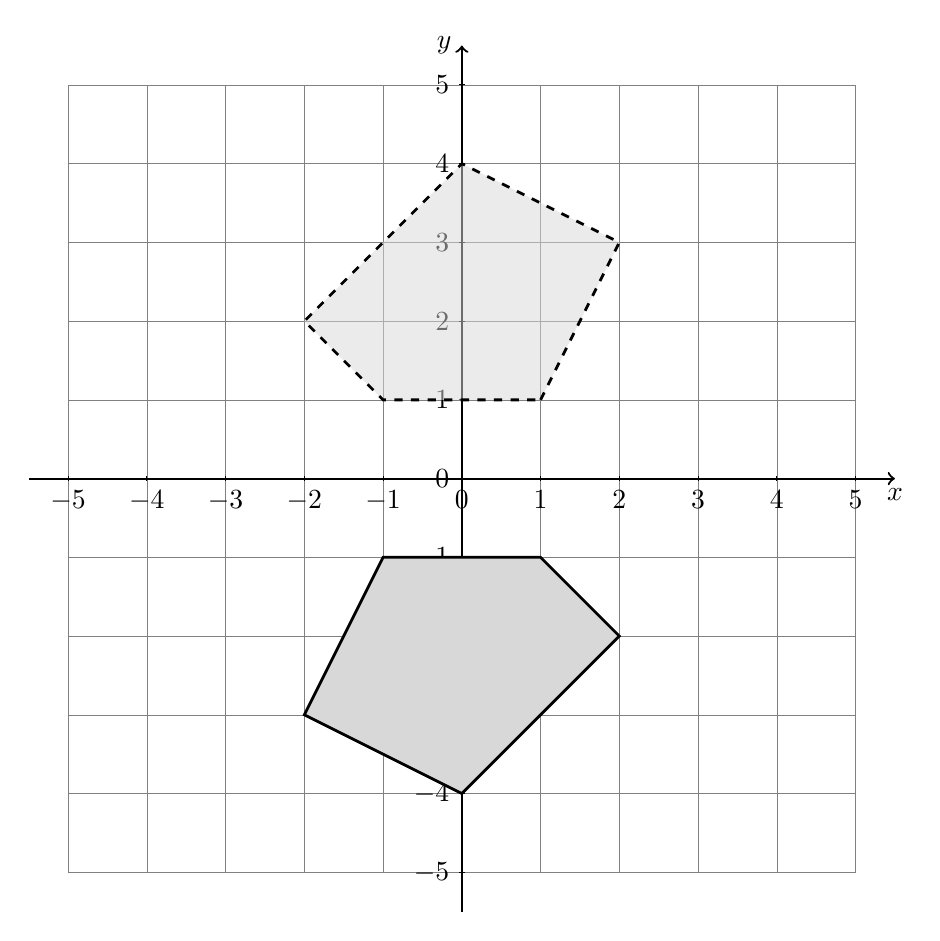
\begin{tikzpicture}[scale=1, transform shape]
    % Define axis scale
    \def\axisLimit{5}

    \definecolor{borderColour}{HTML}{000000}
    \definecolor{fillColour}{HTML}{D8D8D8}

    % Draw grid
    \draw[step=1cm,gray,very thin] (-\axisLimit,-\axisLimit) grid (\axisLimit,\axisLimit);
    
    % Draw axes
    \draw[thick,->] (-\axisLimit-0.5,0) -- (\axisLimit+0.5,0) node[anchor=north] {$x$};
    \draw[thick,->] (0,-\axisLimit-0.5) -- (0,\axisLimit+0.5) node[anchor=east] {$y$};

    % Label x-axis and y-axis
    \foreach \x in {-\axisLimit,...,\axisLimit}
        \draw (\x cm,1pt) -- (\x cm,-1pt) node[anchor=north] {$\x$};
    \foreach \y in {-\axisLimit,...,\axisLimit}
        \draw (1pt,\y cm) -- (-1pt,\y cm) node[anchor=east] {$\y$};

    % Define the center of rotation
    \coordinate (center) at (0,0);

    % Define the vertices for the original irregular polygon
    \coordinate (V1) at (-1,-1);
    \coordinate (V2) at (-2,-3);
    \coordinate (V3) at (0,-4);
    \coordinate (V4) at (2,-2);
    \coordinate (V5) at (1,-1);

    % Draw the original irregular polygon
    \draw[fill=fillColour, draw=borderColour, line width=1pt] (V1) -- (V2) -- (V3) -- (V4) -- (V5) -- cycle;

    % Calculate the new vertices after rotation
    \foreach \angle in {180} {
        \coordinate (V1\angle) at ([rotate around={\angle:(center)}]V1);
        \coordinate (V2\angle) at ([rotate around={\angle:(center)}]V2);
        \coordinate (V3\angle) at ([rotate around={\angle:(center)}]V3);
        \coordinate (V4\angle) at ([rotate around={\angle:(center)}]V4);
        \coordinate (V5\angle) at ([rotate around={\angle:(center)}]V5);
        % Draw the rotated polygon with 50% opacity
        \draw[fill=fillColour, draw=borderColour, line width=1pt, dashed, fill opacity=0.5] 
            (V1\angle) -- (V2\angle) -- (V3\angle) -- (V4\angle) -- (V5\angle) -- cycle;
    }

\end{tikzpicture}

% Q14 (solution (iii))
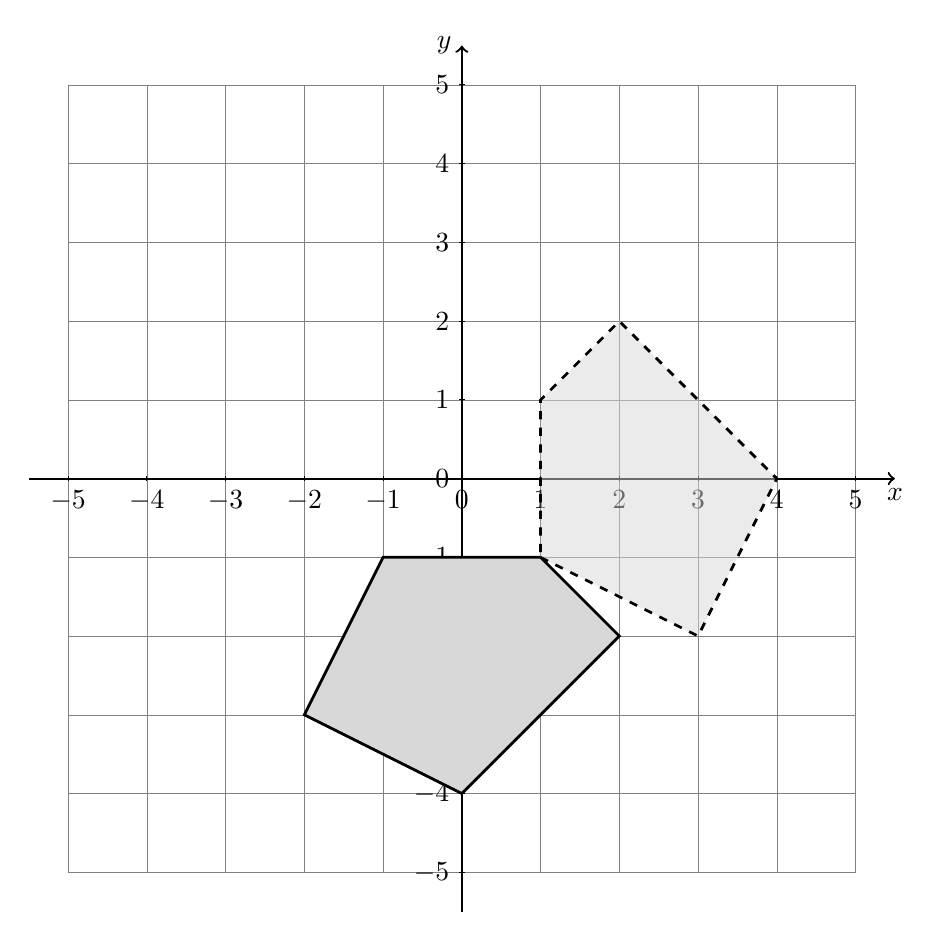
\begin{tikzpicture}[scale=1, transform shape]
    % Define axis scale
    \def\axisLimit{5}

    \definecolor{borderColour}{HTML}{000000}
    \definecolor{fillColour}{HTML}{D8D8D8}

    % Draw grid
    \draw[step=1cm,gray,very thin] (-\axisLimit,-\axisLimit) grid (\axisLimit,\axisLimit);
    
    % Draw axes
    \draw[thick,->] (-\axisLimit-0.5,0) -- (\axisLimit+0.5,0) node[anchor=north] {$x$};
    \draw[thick,->] (0,-\axisLimit-0.5) -- (0,\axisLimit+0.5) node[anchor=east] {$y$};

    % Label x-axis and y-axis
    \foreach \x in {-\axisLimit,...,\axisLimit}
        \draw (\x cm,1pt) -- (\x cm,-1pt) node[anchor=north] {$\x$};
    \foreach \y in {-\axisLimit,...,\axisLimit}
        \draw (1pt,\y cm) -- (-1pt,\y cm) node[anchor=east] {$\y$};

    % Define the center of rotation
    \coordinate (center) at (0,0);

    % Define the vertices for the original irregular polygon
    \coordinate (V1) at (-1,-1);
    \coordinate (V2) at (-2,-3);
    \coordinate (V3) at (0,-4);
    \coordinate (V4) at (2,-2);
    \coordinate (V5) at (1,-1);

    % Draw the original irregular polygon
    \draw[fill=fillColour, draw=borderColour, line width=1pt] (V1) -- (V2) -- (V3) -- (V4) -- (V5) -- cycle;

    % Calculate the new vertices after rotation
    \foreach \angle in {90} {
        \coordinate (V1\angle) at ([rotate around={\angle:(center)}]V1);
        \coordinate (V2\angle) at ([rotate around={\angle:(center)}]V2);
        \coordinate (V3\angle) at ([rotate around={\angle:(center)}]V3);
        \coordinate (V4\angle) at ([rotate around={\angle:(center)}]V4);
        \coordinate (V5\angle) at ([rotate around={\angle:(center)}]V5);
        % Draw the rotated polygon with 50% opacity
        \draw[fill=fillColour, draw=borderColour, line width=1pt, dashed, fill opacity=0.5] 
            (V1\angle) -- (V2\angle) -- (V3\angle) -- (V4\angle) -- (V5\angle) -- cycle;
    }

\end{tikzpicture}

% Q15
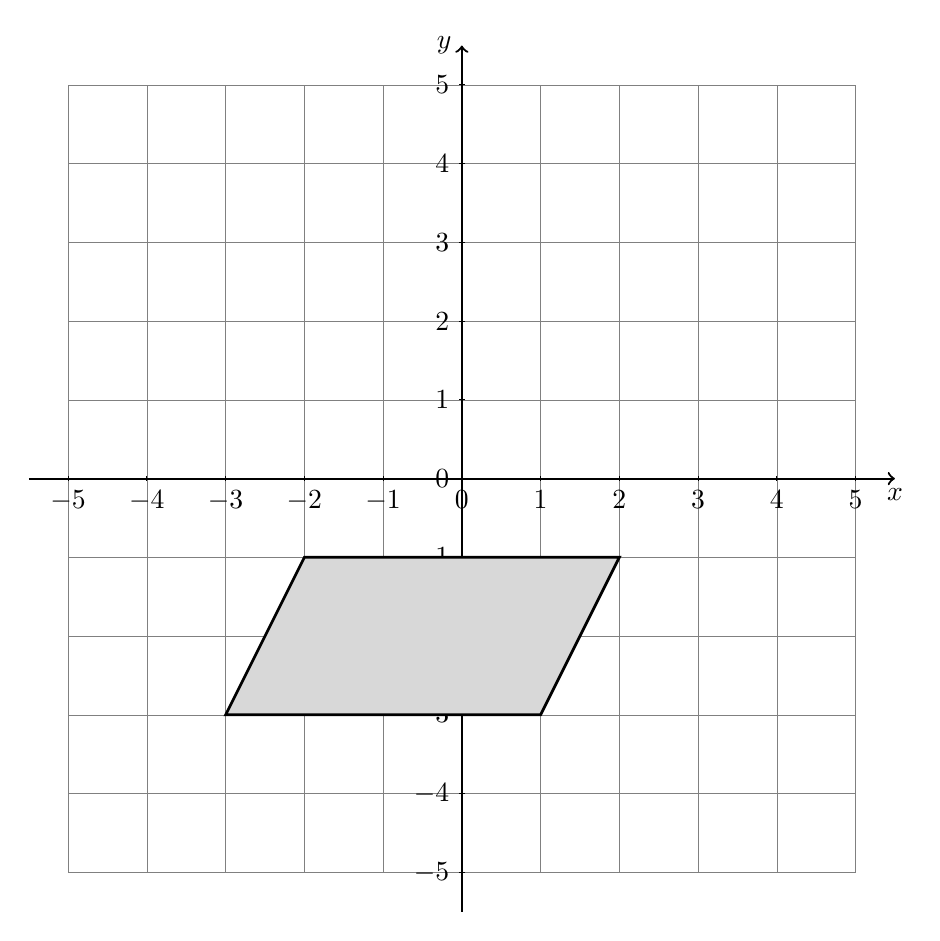
\begin{tikzpicture}[scale=1, transform shape]
    % Define axis scale
    \def\axisLimit{5}

    \definecolor{borderColour}{HTML}{000000}
    \definecolor{fillColour}{HTML}{D8D8D8}

    % Draw grid
    \draw[step=1cm,gray,very thin] (-\axisLimit,-\axisLimit) grid (\axisLimit,\axisLimit);
    
    % Draw axes
    \draw[thick,->] (-\axisLimit-0.5,0) -- (\axisLimit+0.5,0) node[anchor=north] {$x$};
    \draw[thick,->] (0,-\axisLimit-0.5) -- (0,\axisLimit+0.5) node[anchor=east] {$y$};

    % Label x-axis and y-axis
    \foreach \x in {-\axisLimit,...,\axisLimit}
        \draw (\x cm,1pt) -- (\x cm,-1pt) node[anchor=north] {$\x$};
    \foreach \y in {-\axisLimit,...,\axisLimit}
        \draw (1pt,\y cm) -- (-1pt,\y cm) node[anchor=east] {$\y$};

    % Define the center of rotation
    \coordinate (center) at (0,0);

    % Define the vertices for the original trapezium
    \coordinate (A) at (-2,-1);
    \coordinate (B) at (-3,-3);
    \coordinate (C) at (1,-3);
    \coordinate (D) at (2,-1);

    % Draw the original trapezium
    \draw[fill=fillColour, draw=borderColour, line width=1pt] (A) -- (B) -- (C) -- (D) -- cycle;

\end{tikzpicture}

% Q15 (solution (i))
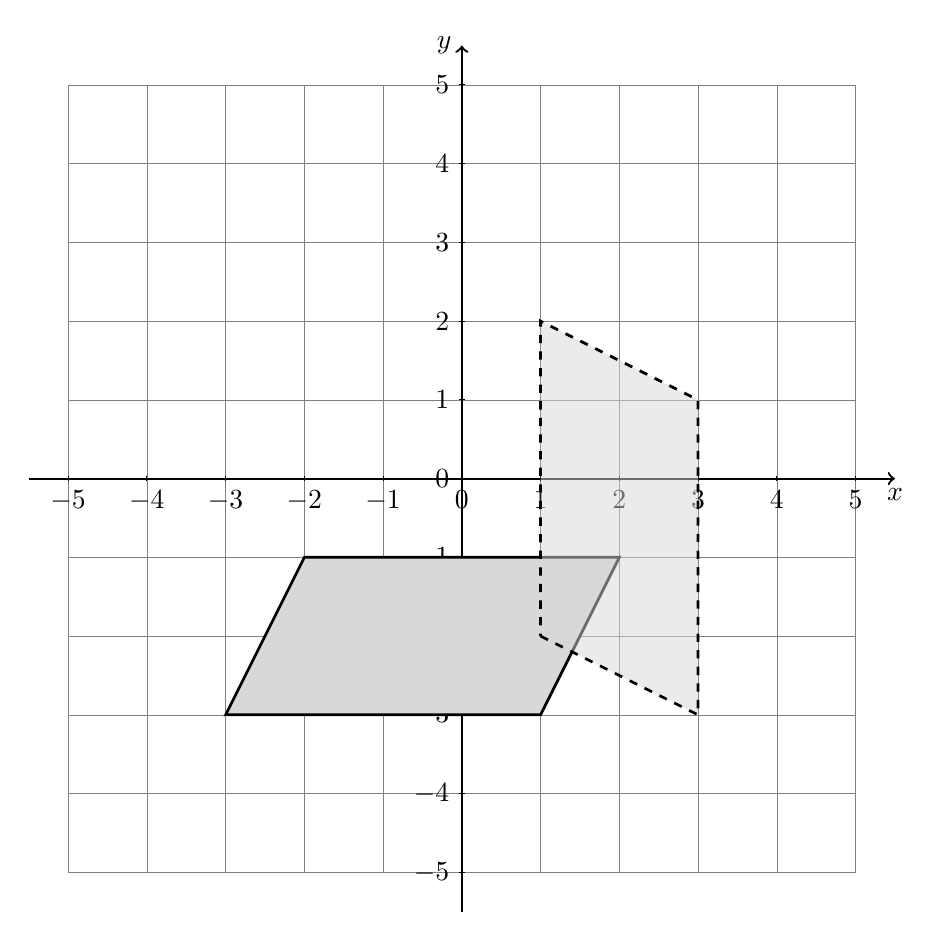
\begin{tikzpicture}[scale=1, transform shape]
    % Define axis scale
    \def\axisLimit{5}

    \definecolor{borderColour}{HTML}{000000}
    \definecolor{fillColour}{HTML}{D8D8D8}

    % Draw grid
    \draw[step=1cm,gray,very thin] (-\axisLimit,-\axisLimit) grid (\axisLimit,\axisLimit);
    
    % Draw axes
    \draw[thick,->] (-\axisLimit-0.5,0) -- (\axisLimit+0.5,0) node[anchor=north] {$x$};
    \draw[thick,->] (0,-\axisLimit-0.5) -- (0,\axisLimit+0.5) node[anchor=east] {$y$};

    % Label x-axis and y-axis
    \foreach \x in {-\axisLimit,...,\axisLimit}
        \draw (\x cm,1pt) -- (\x cm,-1pt) node[anchor=north] {$\x$};
    \foreach \y in {-\axisLimit,...,\axisLimit}
        \draw (1pt,\y cm) -- (-1pt,\y cm) node[anchor=east] {$\y$};

    % Define the center of rotation
    \coordinate (center) at (0,0);

    % Define the vertices for the original trapezium
    \coordinate (A) at (-2,-1);
    \coordinate (B) at (-3,-3);
    \coordinate (C) at (1,-3);
    \coordinate (D) at (2,-1);

    % Draw the original trapezium
    \draw[fill=fillColour, draw=borderColour, line width=1pt] (A) -- (B) -- (C) -- (D) -- cycle;

    % Calculate the new vertices after rotation
    \foreach \angle in {90} {
        \coordinate (A\angle) at ([rotate around={\angle:(center)}]A);
        \coordinate (B\angle) at ([rotate around={\angle:(center)}]B);
        \coordinate (C\angle) at ([rotate around={\angle:(center)}]C);
        \coordinate (D\angle) at ([rotate around={\angle:(center)}]D);
        % Draw the rotated trapezium with 50% opacity
        \draw[fill=fillColour, draw=borderColour, line width=1pt, dashed, fill opacity=0.5] 
            (A\angle) -- (B\angle) -- (C\angle) -- (D\angle) -- cycle;
    }

\end{tikzpicture}

% Q15 (solution (ii))
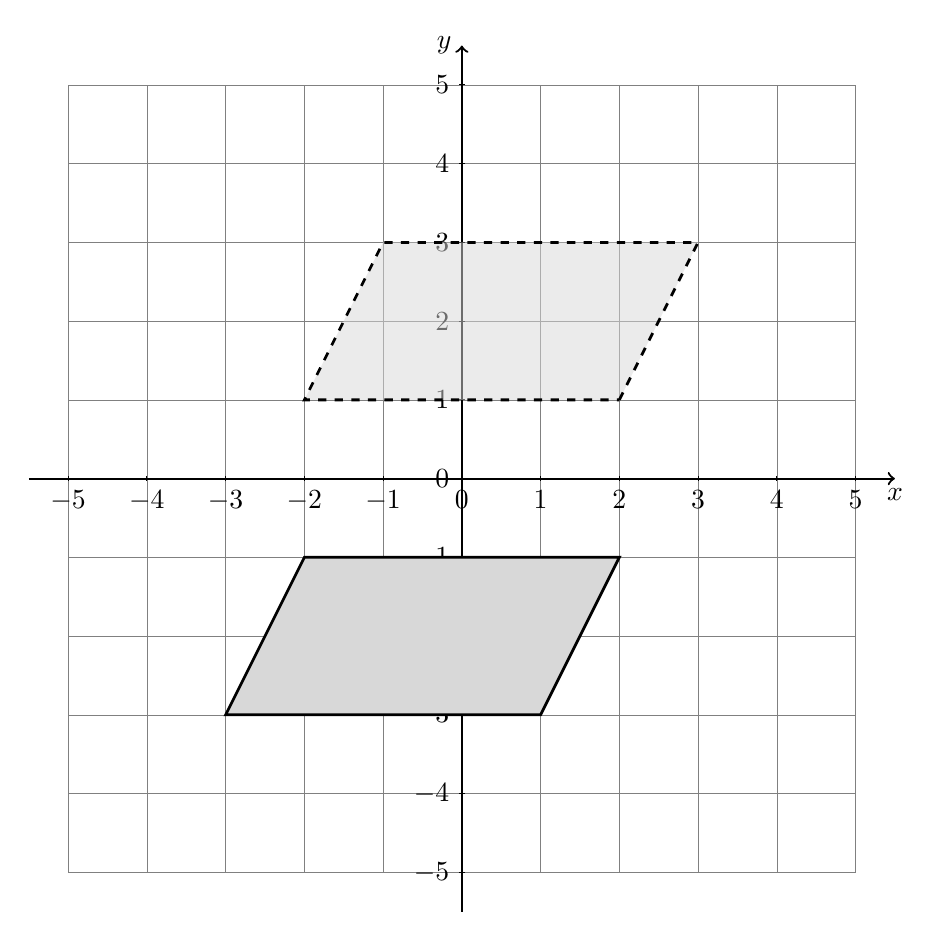
\begin{tikzpicture}[scale=1, transform shape]
    % Define axis scale
    \def\axisLimit{5}

    \definecolor{borderColour}{HTML}{000000}
    \definecolor{fillColour}{HTML}{D8D8D8}

    % Draw grid
    \draw[step=1cm,gray,very thin] (-\axisLimit,-\axisLimit) grid (\axisLimit,\axisLimit);
    
    % Draw axes
    \draw[thick,->] (-\axisLimit-0.5,0) -- (\axisLimit+0.5,0) node[anchor=north] {$x$};
    \draw[thick,->] (0,-\axisLimit-0.5) -- (0,\axisLimit+0.5) node[anchor=east] {$y$};

    % Label x-axis and y-axis
    \foreach \x in {-\axisLimit,...,\axisLimit}
        \draw (\x cm,1pt) -- (\x cm,-1pt) node[anchor=north] {$\x$};
    \foreach \y in {-\axisLimit,...,\axisLimit}
        \draw (1pt,\y cm) -- (-1pt,\y cm) node[anchor=east] {$\y$};

    % Define the center of rotation
    \coordinate (center) at (0,0);

    % Define the vertices for the original trapezium
    \coordinate (A) at (-2,-1);
    \coordinate (B) at (-3,-3);
    \coordinate (C) at (1,-3);
    \coordinate (D) at (2,-1);

    % Draw the original trapezium
    \draw[fill=fillColour, draw=borderColour, line width=1pt] (A) -- (B) -- (C) -- (D) -- cycle;

    % Calculate the new vertices after rotation
    \foreach \angle in {180} {
        \coordinate (A\angle) at ([rotate around={\angle:(center)}]A);
        \coordinate (B\angle) at ([rotate around={\angle:(center)}]B);
        \coordinate (C\angle) at ([rotate around={\angle:(center)}]C);
        \coordinate (D\angle) at ([rotate around={\angle:(center)}]D);
        % Draw the rotated trapezium with 50% opacity
        \draw[fill=fillColour, draw=borderColour, line width=1pt, dashed, fill opacity=0.5] 
            (A\angle) -- (B\angle) -- (C\angle) -- (D\angle) -- cycle;
    }

\end{tikzpicture}

% Q15 (solution (iii))
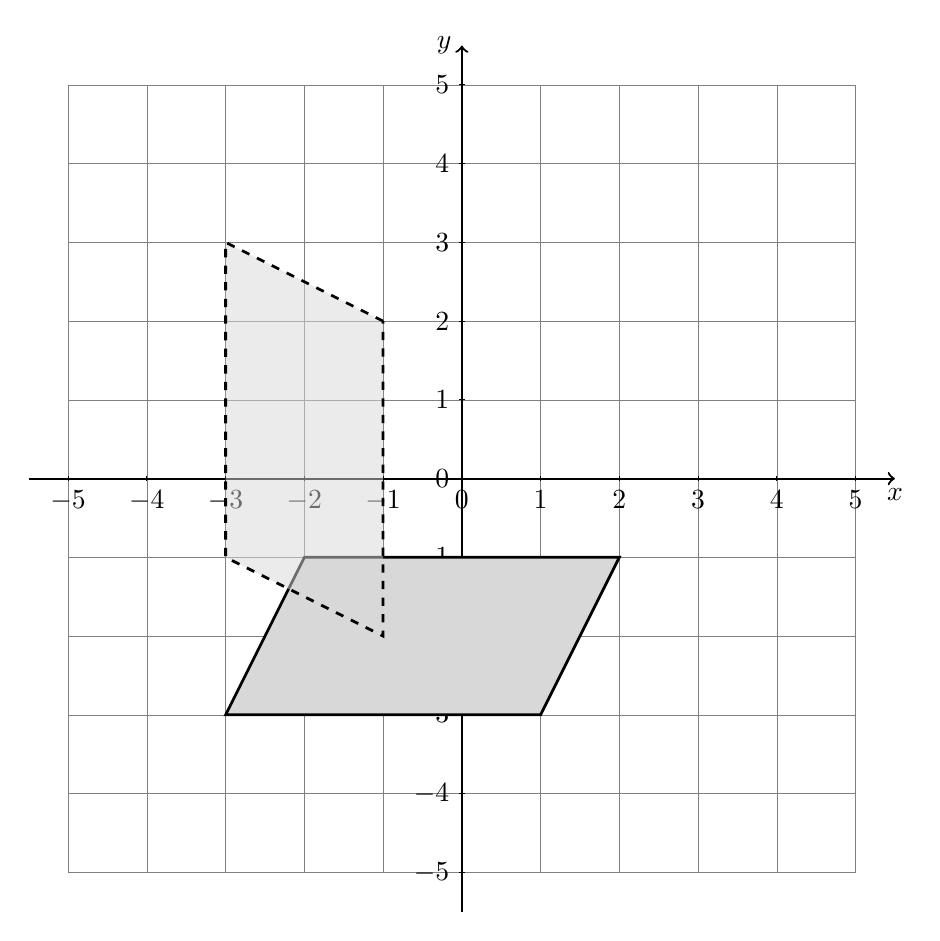
\begin{tikzpicture}[scale=1, transform shape]
    % Define axis scale
    \def\axisLimit{5}

    \definecolor{borderColour}{HTML}{000000}
    \definecolor{fillColour}{HTML}{D8D8D8}

    % Draw grid
    \draw[step=1cm,gray,very thin] (-\axisLimit,-\axisLimit) grid (\axisLimit,\axisLimit);
    
    % Draw axes
    \draw[thick,->] (-\axisLimit-0.5,0) -- (\axisLimit+0.5,0) node[anchor=north] {$x$};
    \draw[thick,->] (0,-\axisLimit-0.5) -- (0,\axisLimit+0.5) node[anchor=east] {$y$};

    % Label x-axis and y-axis
    \foreach \x in {-\axisLimit,...,\axisLimit}
        \draw (\x cm,1pt) -- (\x cm,-1pt) node[anchor=north] {$\x$};
    \foreach \y in {-\axisLimit,...,\axisLimit}
        \draw (1pt,\y cm) -- (-1pt,\y cm) node[anchor=east] {$\y$};

    % Define the center of rotation
    \coordinate (center) at (0,0);

    % Define the vertices for the original trapezium
    \coordinate (A) at (-2,-1);
    \coordinate (B) at (-3,-3);
    \coordinate (C) at (1,-3);
    \coordinate (D) at (2,-1);

    % Draw the original trapezium
    \draw[fill=fillColour, draw=borderColour, line width=1pt] (A) -- (B) -- (C) -- (D) -- cycle;

    % Calculate the new vertices after rotation
    \foreach \angle in {270} {
        \coordinate (A\angle) at ([rotate around={\angle:(center)}]A);
        \coordinate (B\angle) at ([rotate around={\angle:(center)}]B);
        \coordinate (C\angle) at ([rotate around={\angle:(center)}]C);
        \coordinate (D\angle) at ([rotate around={\angle:(center)}]D);
        % Draw the rotated trapezium with 50% opacity
        \draw[fill=fillColour, draw=borderColour, line width=1pt, dashed, fill opacity=0.5] 
            (A\angle) -- (B\angle) -- (C\angle) -- (D\angle) -- cycle;
    }

\end{tikzpicture}

% Q16
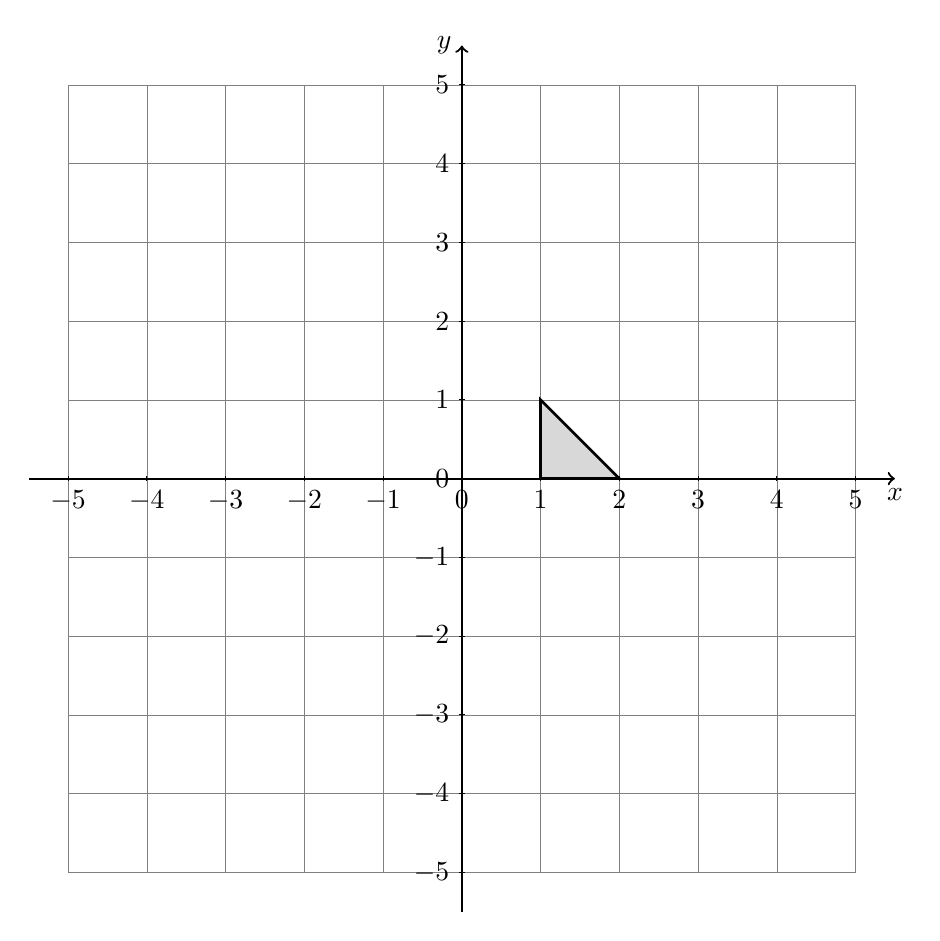
\begin{tikzpicture}[scale=1, transform shape]
    % Define axis scale
    \def\axisLimit{5}

    \definecolor{borderColour}{HTML}{000000}
    \definecolor{fillColour}{HTML}{D8D8D8}

    % Draw grid
    \draw[step=1cm,gray,very thin] (-\axisLimit,-\axisLimit) grid (\axisLimit,\axisLimit);
    
    % Draw axes
    \draw[thick,->] (-\axisLimit-0.5,0) -- (\axisLimit+0.5,0) node[anchor=north] {$x$};
    \draw[thick,->] (0,-\axisLimit-0.5) -- (0,\axisLimit+0.5) node[anchor=east] {$y$};

    % Label x-axis and y-axis
    \foreach \x in {-\axisLimit,...,\axisLimit}
        \draw (\x cm,1pt) -- (\x cm,-1pt) node[anchor=north] {$\x$};
    \foreach \y in {-\axisLimit,...,\axisLimit}
        \draw (1pt,\y cm) -- (-1pt,\y cm) node[anchor=east] {$\y$};

    % Define the center of enlargement (origin)
    \coordinate (COE) at (0,0);

    % Define the vertices for the original right-angled triangle
    \coordinate (A) at (1,0);
    \coordinate (B) at (1,1);
    \coordinate (C) at (2,0);

    % Draw the original right-angled triangle
    \draw[fill=fillColour, draw=borderColour, line width=1pt] (A) -- (B) -- (C) -- cycle;
\end{tikzpicture}

% Q16 (solution)
\begin{tikzpicture}[scale=1, transform shape]
    % Define axis scale
    \def\axisLimit{5}

    \definecolor{borderColour}{HTML}{000000}
    \definecolor{fillColour}{HTML}{D8D8D8}

    % Draw grid
    \draw[step=1cm,gray,very thin] (-\axisLimit,-\axisLimit) grid (\axisLimit,\axisLimit);
    
    % Draw axes
    \draw[thick,->] (-\axisLimit-0.5,0) -- (\axisLimit+0.5,0) node[anchor=north] {$x$};
    \draw[thick,->] (0,-\axisLimit-0.5) -- (0,\axisLimit+0.5) node[anchor=east] {$y$};

    % Label x-axis and y-axis
    \foreach \x in {-\axisLimit,...,\axisLimit}
        \draw (\x cm,1pt) -- (\x cm,-1pt) node[anchor=north] {$\x$};
    \foreach \y in {-\axisLimit,...,\axisLimit}
        \draw (1pt,\y cm) -- (-1pt,\y cm) node[anchor=east] {$\y$};

    % Define the center of enlargement (origin)
    \coordinate (COE) at (0,0);

    % Define the vertices for the original right-angled triangle
    \coordinate (A) at (1,0);
    \coordinate (B) at (1,1);
    \coordinate (C) at (2,0);

    % Draw the original right-angled triangle
    \draw[fill=fillColour, draw=borderColour, line width=1pt] (A) -- (B) -- (C) -- cycle;

    % Calculate the new vertices after enlargement
    \coordinate (A') at ($(center)!2!(A)$);
    \coordinate (B') at ($(center)!2!(B)$);
    \coordinate (C') at ($(center)!2!(C)$);

    % Draw the enlarged triangle
    \draw[fill=fillColour, draw=borderColour, line width=1pt, dashed, fill opacity=0.5] (A') -- (B') -- (C') -- cycle;

    % Draw red dashed lines
    \draw[dashed, line width=1pt, red] (COE) -- (A');
    \draw[dashed, line width=1pt, red] (COE) -- (B');
    \draw[dashed, line width=1pt, red] (COE) -- (C');

\end{tikzpicture}

% Q17
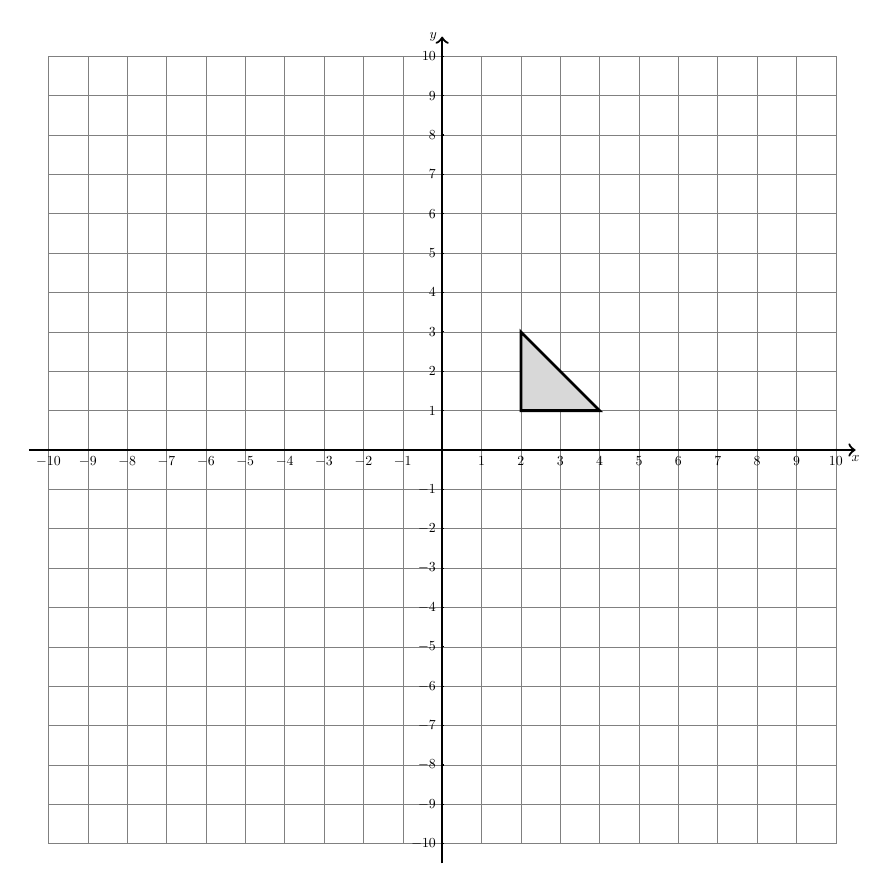
\begin{tikzpicture}[scale=0.5, transform shape]
    % Define axis scale
    \def\axisLimit{5}

    \definecolor{borderColour}{HTML}{000000}
    \definecolor{fillColour}{HTML}{D8D8D8}

    % Draw grid
    \draw[step=1cm,gray,very thin] (-10,-10) grid (10,10);
    
    % Draw axes
    \draw[thick,->] (-10.5,0) -- (10.5,0) node[anchor=north] {$x$};
    \draw[thick,->] (0,-10.5) -- (0,10.5) node[anchor=east] {$y$};

    % Label x-axis and y-axis
    \foreach \x in {-10,...,-1,1,2,...,10}
        \draw (\x cm,1pt) -- (\x cm,-1pt) node[anchor=north] {$\x$};
    \foreach \y in {-10,...,-1,1,2,...,10}
        \draw (1pt,\y cm) -- (-1pt,\y cm) node[anchor=east] {$\y$};

    % Define the center of enlargement (COE) and scale factor
    \def\scaleFactor{2}
    \coordinate (COE) at (7,7);

    % Define the vertices for the original right-angled triangle
    \coordinate (A) at (2,1);
    \coordinate (B) at (2,3);
    \coordinate (C) at (4,1);

    % Draw the original right-angled triangle
    \draw[fill=fillColour, draw=borderColour, line width=1pt] (A) -- (B) -- (C) -- cycle;

\end{tikzpicture}

% Q17 (solution)
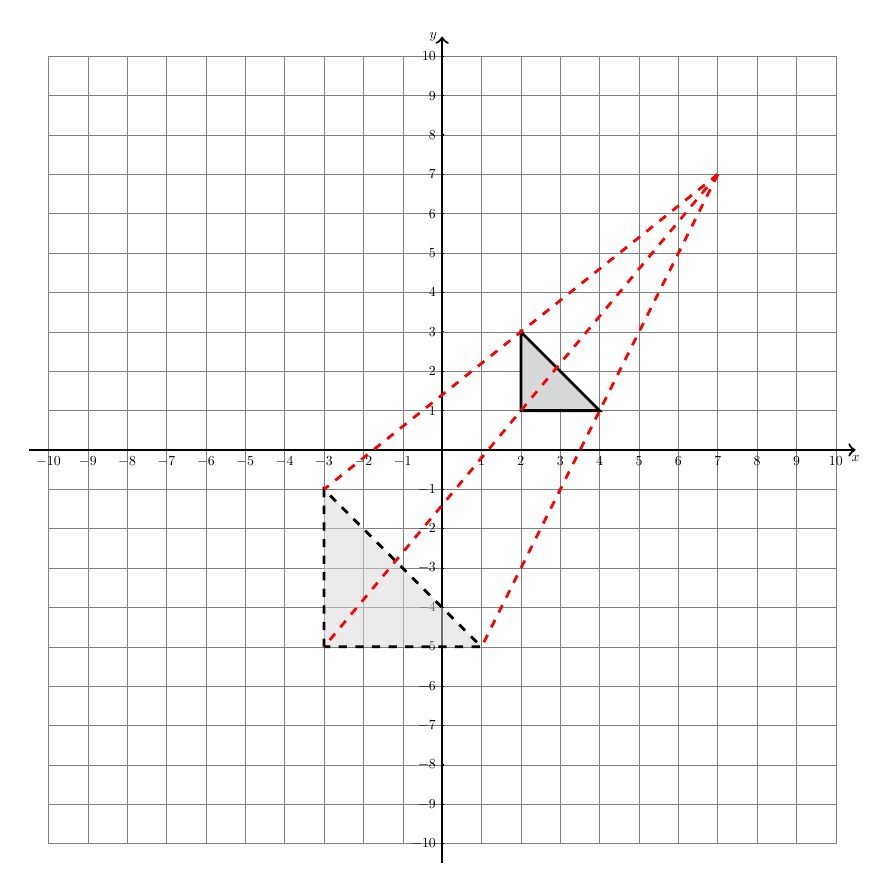
\begin{tikzpicture}[scale=0.5, transform shape]
    % Define axis scale
    \def\axisLimit{5}

    \definecolor{borderColour}{HTML}{000000}
    \definecolor{fillColour}{HTML}{D8D8D8}

    % Draw grid
    \draw[step=1cm,gray,very thin] (-10,-10) grid (10,10);
    
    % Draw axes
    \draw[thick,->] (-10.5,0) -- (10.5,0) node[anchor=north] {$x$};
    \draw[thick,->] (0,-10.5) -- (0,10.5) node[anchor=east] {$y$};

    % Label x-axis and y-axis
    \foreach \x in {-10,...,-1,1,2,...,10}
        \draw (\x cm,1pt) -- (\x cm,-1pt) node[anchor=north] {$\x$};
    \foreach \y in {-10,...,-1,1,2,...,10}
        \draw (1pt,\y cm) -- (-1pt,\y cm) node[anchor=east] {$\y$};

    % Define the center of enlargement (COE) and scale factor
    \def\scaleFactor{2}
    \coordinate (COE) at (7,7);

    % Define the vertices for the original right-angled triangle
    \coordinate (A) at (2,1);
    \coordinate (B) at (2,3);
    \coordinate (C) at (4,1);

    % Draw the original right-angled triangle
    \draw[fill=fillColour, draw=borderColour, line width=1pt] (A) -- (B) -- (C) -- cycle;

    % Calculate the new vertices after enlargement
    \coordinate (A') at ($(COE)!\scaleFactor!(A)$);
    \coordinate (B') at ($(COE)!\scaleFactor!(B)$);
    \coordinate (C') at ($(COE)!\scaleFactor!(C)$);

    % Draw the enlarged triangle
    \draw[fill=fillColour, draw=borderColour, line width=1pt, dashed, fill opacity=0.5] (A') -- (B') -- (C') -- cycle;

    % Draw red dashed lines
    \draw[dashed, line width=1pt, red] (COE) -- (A');
    \draw[dashed, line width=1pt, red] (COE) -- (B');
    \draw[dashed, line width=1pt, red] (COE) -- (C');

\end{tikzpicture}

% Q18
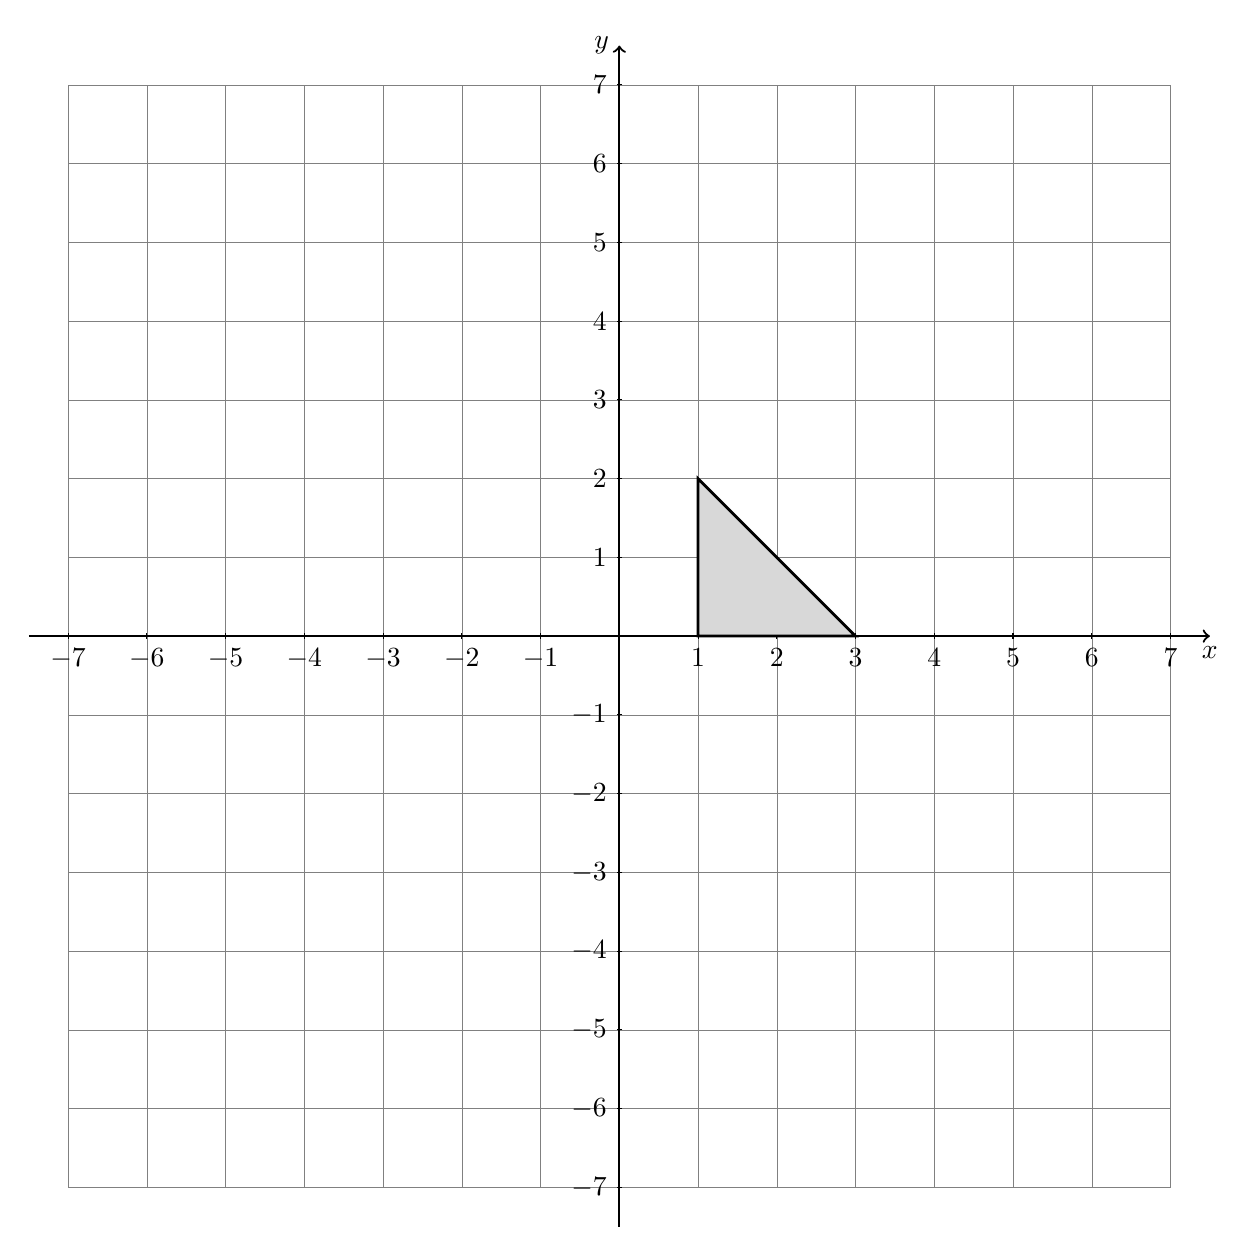
\begin{tikzpicture}[scale=1, transform shape]

    % Define the axis limit
    \def\axisLimit{7}

    \definecolor{borderColour}{HTML}{000000}
    \definecolor{fillColour}{HTML}{D8D8D8}

    % Define the scale factor and center of enlargement
    \def\scaleFactor{2.5}
    \coordinate (COE) at (2,-1);

    % Draw grid
    \draw[step=1cm,gray,very thin] (-\axisLimit,-\axisLimit) grid (\axisLimit,\axisLimit);
    
    % Draw axes
    \draw[thick,->] (-\axisLimit-0.5,0) -- (\axisLimit+0.5,0) node[anchor=north] {$x$};
    \draw[thick,->] (0,-\axisLimit-0.5) -- (0,\axisLimit+0.5) node[anchor=east] {$y$};

    % Label x-axis and y-axis
    \foreach \x in {-\axisLimit,...,-1,1,2,...,\axisLimit}
        \draw (\x cm,1pt) -- (\x cm,-1pt) node[anchor=north] {$\x$};
    \foreach \y in {-\axisLimit,...,-1,1,2,...,\axisLimit}
        \draw (1pt,\y cm) -- (-1pt,\y cm) node[anchor=east] {$\y$};
        
    % Define the vertices for the original right-angled triangle
    \coordinate (A) at (1,0);
    \coordinate (B) at (1,2);
    \coordinate (C) at (3,0);

    % Draw the original right-angled triangle
    \draw[fill=fillColour, draw=borderColour, line width=1pt] (A) -- (B) -- (C) -- cycle;
    
\end{tikzpicture}

% Q18 (solution)
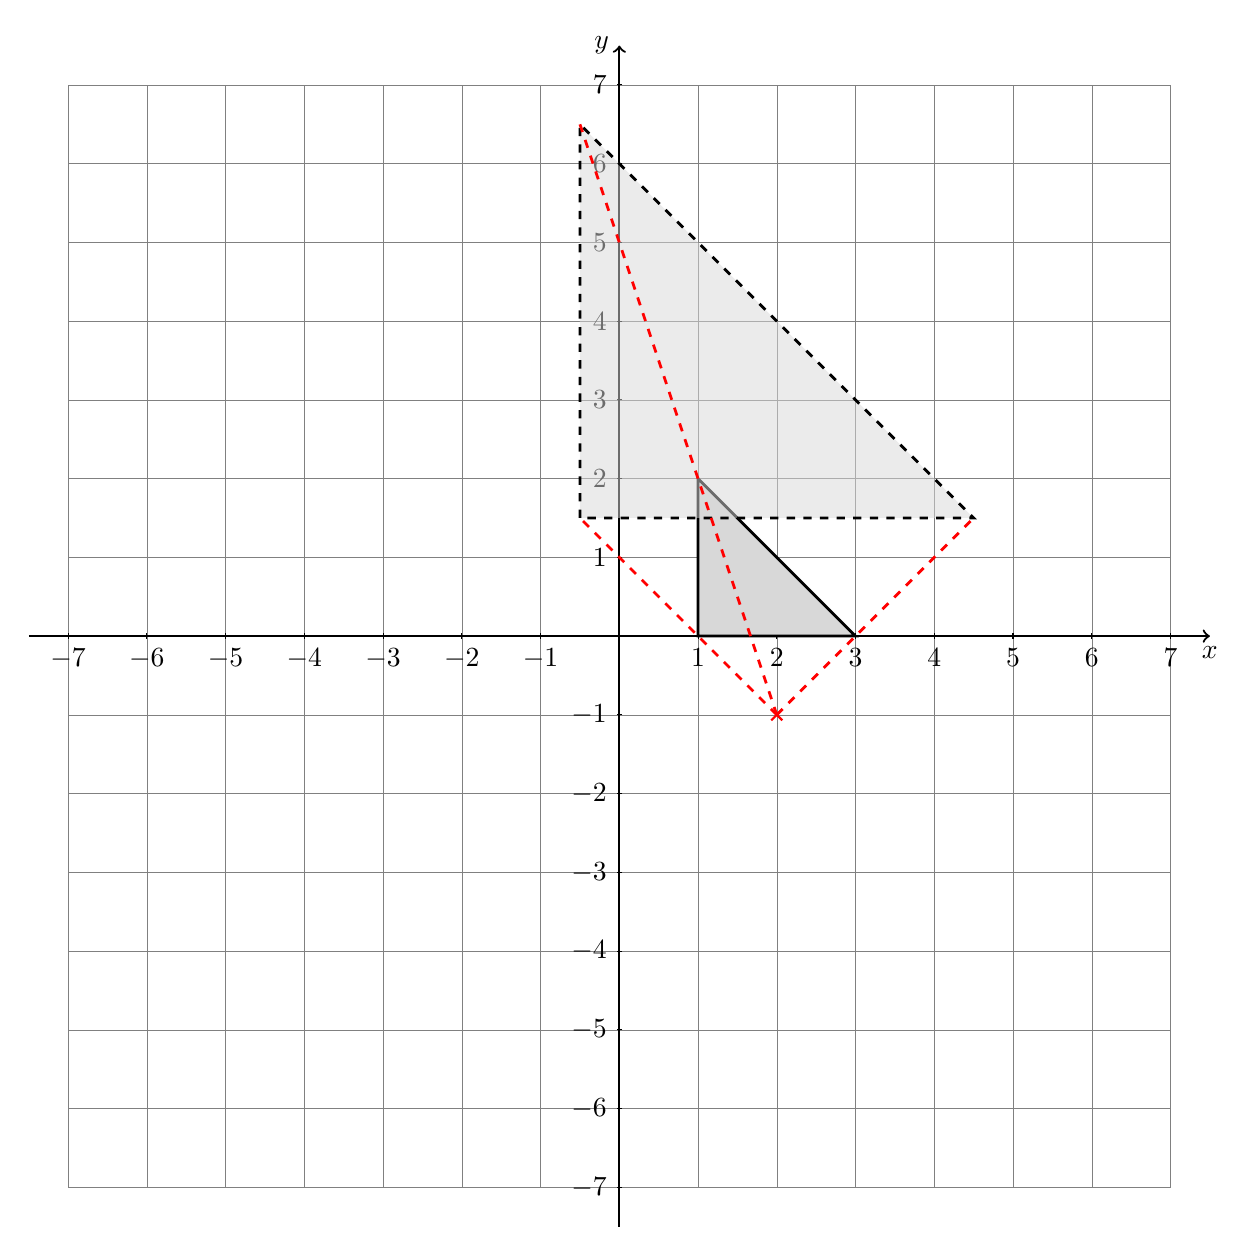
\begin{tikzpicture}[scale=1, transform shape]

    % Define the axis limit
    \def\axisLimit{7}

    \definecolor{borderColour}{HTML}{000000}
    \definecolor{fillColour}{HTML}{D8D8D8}

    % Define the scale factor and center of enlargement
    \def\scaleFactor{2.5}
    \coordinate (COE) at (2,-1);

    % Draw grid
    \draw[step=1cm,gray,very thin] (-\axisLimit,-\axisLimit) grid (\axisLimit,\axisLimit);
    
    % Draw axes
    \draw[thick,->] (-\axisLimit-0.5,0) -- (\axisLimit+0.5,0) node[anchor=north] {$x$};
    \draw[thick,->] (0,-\axisLimit-0.5) -- (0,\axisLimit+0.5) node[anchor=east] {$y$};

    % Label x-axis and y-axis
    \foreach \x in {-\axisLimit,...,-1,1,2,...,\axisLimit}
        \draw (\x cm,1pt) -- (\x cm,-1pt) node[anchor=north] {$\x$};
    \foreach \y in {-\axisLimit,...,-1,1,2,...,\axisLimit}
        \draw (1pt,\y cm) -- (-1pt,\y cm) node[anchor=east] {$\y$};

    % Draw the center of enlargement
    \draw[red, thick] (COE) node[cross out, draw=red, inner sep=2pt, outer sep=0pt] {};
    
    % Define the vertices for the original right-angled triangle
    \coordinate (A) at (1,0);
    \coordinate (B) at (1,2);
    \coordinate (C) at (3,0);

    % Draw the original right-angled triangle
    \draw[fill=fillColour, draw=borderColour, line width=1pt] (A) -- (B) -- (C) -- cycle;

    % Calculate the new vertices after enlargement
    \coordinate (A') at ($(COE)!\scaleFactor!(A)$);
    \coordinate (B') at ($(COE)!\scaleFactor!(B)$);
    \coordinate (C') at ($(COE)!\scaleFactor!(C)$);

    % Draw the enlarged triangle
    \draw[fill=fillColour, draw=borderColour, line width=1pt, dashed, fill opacity=0.5] (A') -- (B') -- (C') -- cycle;

    % Draw red dashed lines
    \draw[dashed, line width=1pt, red] (COE) -- (A');
    \draw[dashed, line width=1pt, red] (COE) -- (B');
    \draw[dashed, line width=1pt, red] (COE) -- (C');
    
\end{tikzpicture}

% Q19
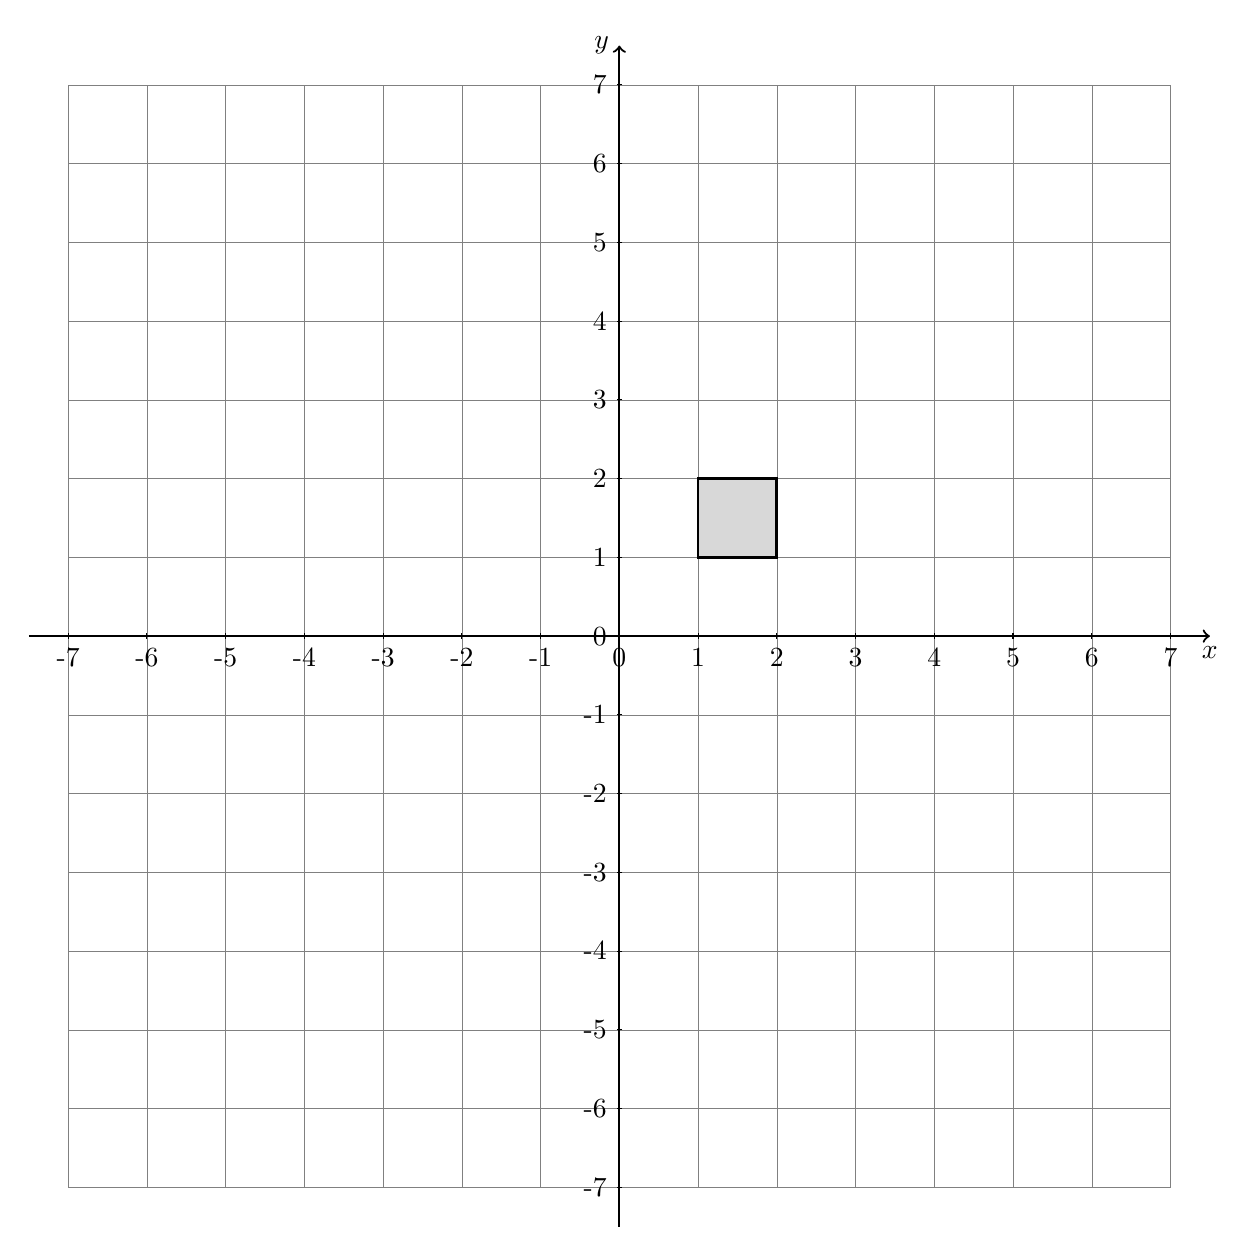
\begin{tikzpicture}[scale=1, transform shape]
    \definecolor{borderColour}{HTML}{000000}
    \definecolor{fillColour}{HTML}{D8D8D8}

    \def\axisLimit{7}
    \def\scaleFactor{3} % Adjusted scale factor for visibility within the grid
    \coordinate (COE) at (0,0); % Center of enlargement at the origin

    % Draw grid
    \draw[step=1cm,gray,very thin] (-\axisLimit,-\axisLimit) grid (\axisLimit,\axisLimit);
    
    % Draw axes
    \draw[thick,->] (-\axisLimit-0.5,0) -- (\axisLimit+0.5,0) node[anchor=north] {$x$};
    \draw[thick,->] (0,-\axisLimit-0.5) -- (0,\axisLimit+0.5) node[anchor=east] {$y$};

    % Label x-axis and y-axis
    \foreach \x in {-\axisLimit,...,\axisLimit}
        \draw (\x cm,1pt) -- (\x cm,-1pt) node[anchor=north] {\x};
    \foreach \y in {-\axisLimit,...,\axisLimit}
        \draw (1pt,\y cm) -- (-1pt,\y cm) node[anchor=east] {\y};

    % Define the vertices for the original rectangle
    \coordinate (A) at (1,1);
    \coordinate (B) at (2,1);
    \coordinate (C) at (2,2);
    \coordinate (D) at (1,2);

    % Draw the original rectangle
    \draw[fill=fillColour, draw=borderColour, line width=1pt] (A) -- (B) -- (C) -- (D) -- cycle;
    
\end{tikzpicture}

% Q19 (solution)
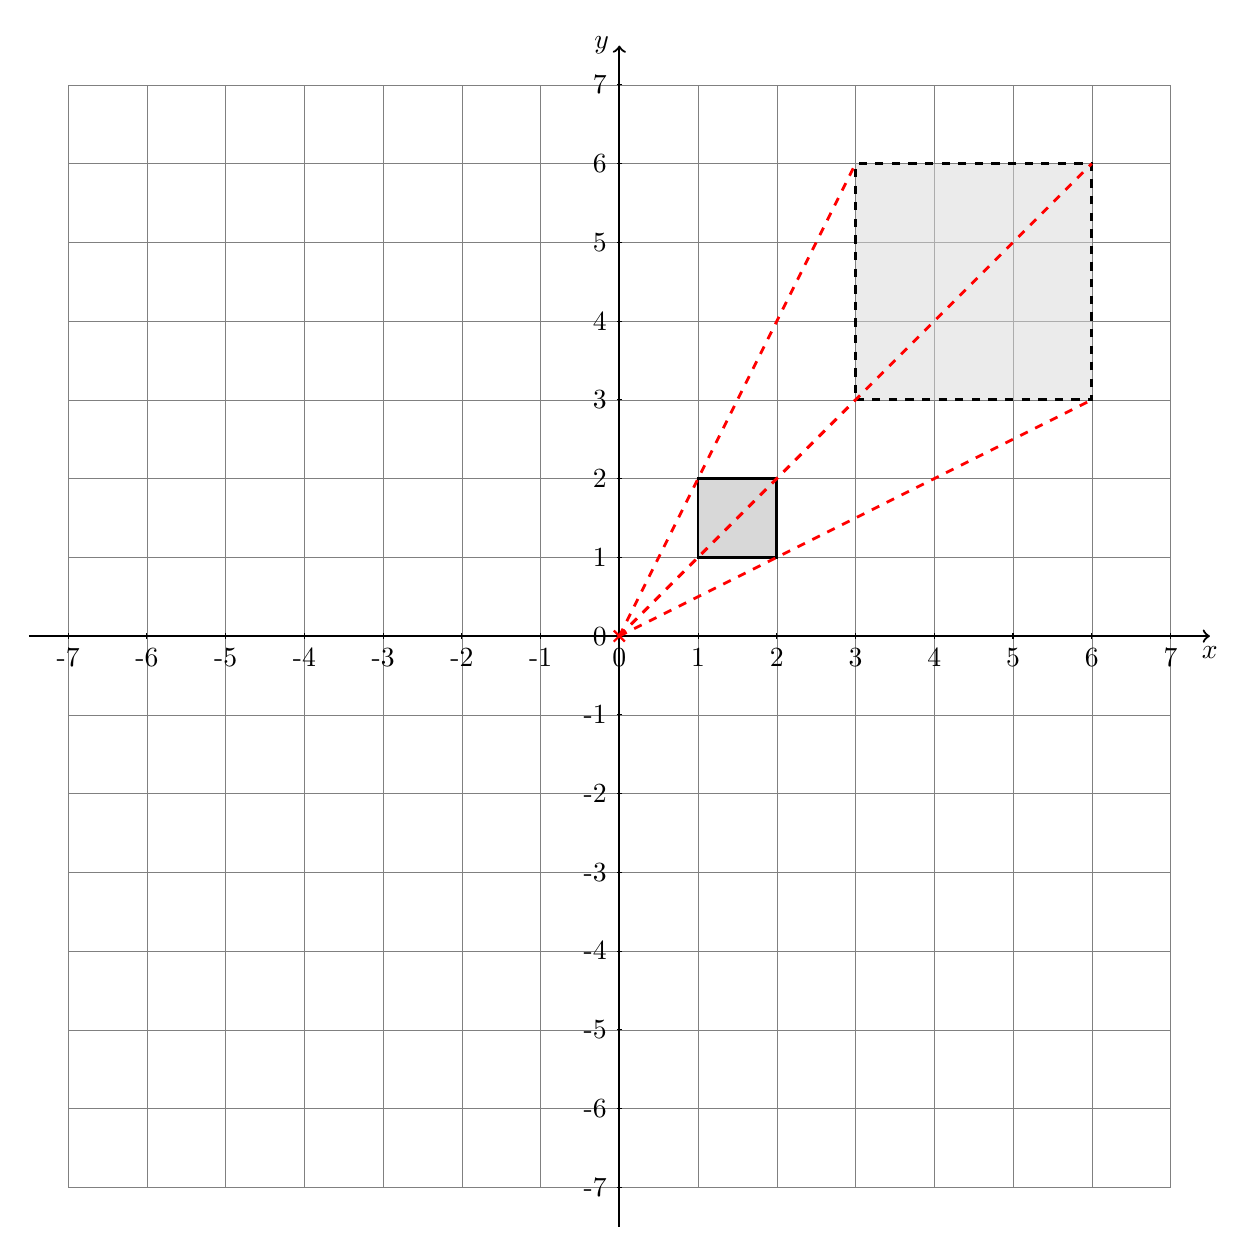
\begin{tikzpicture}[scale=1, transform shape]
    \definecolor{borderColour}{HTML}{000000}
    \definecolor{fillColour}{HTML}{D8D8D8}

    \def\axisLimit{7}
    \def\scaleFactor{3} % Adjusted scale factor for visibility within the grid
    \coordinate (COE) at (0,0); % Center of enlargement at the origin

    % Draw grid
    \draw[step=1cm,gray,very thin] (-\axisLimit,-\axisLimit) grid (\axisLimit,\axisLimit);
    
    % Draw axes
    \draw[thick,->] (-\axisLimit-0.5,0) -- (\axisLimit+0.5,0) node[anchor=north] {$x$};
    \draw[thick,->] (0,-\axisLimit-0.5) -- (0,\axisLimit+0.5) node[anchor=east] {$y$};

    % Label x-axis and y-axis
    \foreach \x in {-\axisLimit,...,\axisLimit}
        \draw (\x cm,1pt) -- (\x cm,-1pt) node[anchor=north] {\x};
    \foreach \y in {-\axisLimit,...,\axisLimit}
        \draw (1pt,\y cm) -- (-1pt,\y cm) node[anchor=east] {\y};

    % Draw the center of enlargement
    \draw[red, thick] (COE) node[cross out, draw=red, inner sep=2pt, outer sep=0pt] {};

    % Define the vertices for the original rectangle
    \coordinate (A) at (1,1);
    \coordinate (B) at (2,1);
    \coordinate (C) at (2,2);
    \coordinate (D) at (1,2);

    % Draw the original rectangle
    \draw[fill=fillColour, draw=borderColour, line width=1pt] (A) -- (B) -- (C) -- (D) -- cycle;

    % Solution Materials
    
    % Calculate the new vertices after enlargement
    \coordinate (A') at ($(COE)!\scaleFactor!(A)$);
    \coordinate (B') at ($(COE)!\scaleFactor!(B)$);
    \coordinate (C') at ($(COE)!\scaleFactor!(C)$);
    \coordinate (D') at ($(COE)!\scaleFactor!(D)$);

    % Draw the enlarged rectangle
    \draw[fill=fillColour, draw=borderColour, line width=1pt, dashed, fill opacity=0.5] (A') -- (B') -- (C') -- (D') -- cycle;

    % Draw red dashed lines connecting original vertices to the enlarged vertices
    \draw[dashed, line width=1pt, red] (COE) -- (A');
    \draw[dashed, line width=1pt, red] (COE) -- (B');
    \draw[dashed, line width=1pt, red] (COE) -- (C');
    \draw[dashed, line width=1pt, red] (COE) -- (D');
    
\end{tikzpicture}

\end{document}
